\documentclass[cn,11pt]{elegantbook}

\title{\,量子场论笔记}
\subtitle{Notes on Quantum Field Theory}

\author{兴趣使然的场论爱好者}
%\bioinfo{录入}{渤海玉兔}
%\institute{Elegant\LaTeX{} Program}
\date{\today}
%\version{3.10}


\extrainfo{The effort to understand the universe is one of the very few things which lifts human life a little above the level of farce and gives it some of the grace of tragedy. --- Steven Weinberg}

%\logo{logo-blue.png}
\cover{Particle.jpeg}

% 本文档命令
%\usepackage[lcgreekalpha]{stix2}
\usepackage{array}
\usepackage{dsfont}
\usepackage{tensor}
%\usepackage[super,square]{natbib}

\usepackage{pgfplots}
\usepgfplotslibrary{polar}
     \usepgflibrary{shapes.geometric}
     \usetikzlibrary{calc}

     \usepackage[perpage]{manyfoot}
     \DeclareNewFootnote{B}[fnsymbol]   %% for weinberg only

%\xeCJKsetup{PunctStyle=quanjiao}
  

\allowdisplaybreaks[4]

 \definecolor{foo}{RGB}{173,34,48}
%+++++++++++++++++++++++数学字体的设置++++++++++++++++++++++++++++++++++++++++%
\newcommand{\me}{\mathrm{e}}  % for math e
\newcommand{\mi}{\mathrm{i}} % for math i
\newcommand{\dif}{\mathrm{d}} %for differential operator d
\newcommand{\cvec}[1]{\!\vec{\,#1}}
\newcommand{\Ptimes}{\,\overset{\otimes }{,}\,}
\DeclareSymbolFont{lettersA}{U}{txmia}{m}{it}
\DeclareMathSymbol{\piup}{\mathord}{lettersA}{25}
 \DeclareMathSymbol{\muup}{\mathord}{lettersA}{22}
 \DeclareMathSymbol{\deltaup}{\mathord}{lettersA}{14}
 \newcommand{\uppi}{\piup}
\newcommand{\ccr}[1]{\makecell{{\color{#1}\rule{1cm}{1cm}}}}

\newcommand{\kai}{\kaishu} % for weinberg only

\newcommand{\hei}{\heiti} % for weinberg only

\DeclareFontEncoding{LS1}{}{}
\DeclareFontSubstitution{LS1}{stix}{m}{n}
\DeclareSymbolFont{symbols2}{LS1}{stixfrak}{m}{n}
\DeclareMathSymbol{\typecolon}{\mathbin}{symbols2}{"25}
% 修改目录深度
\setcounter{tocdepth}{2}

\begin{document}

\maketitle
\frontmatter
\mainmatter

\tableofcontents


%
\renewcommand*\thesection{\arabic{section}}
\setcounter{section}{0}%更改chapter的计数器值
%\numberwithin{equation}{chapter}%公式计数器从属于节计数器
\numberwithin{equation}{section}%公式计数器从属于节计数器
\numberwithin{figure}{chapter}%图计数器从属于节计数器
%\renewcommand*\thefigure{\arabic{section}}
\setcounter{chapter}{0}


\chapter[瞬子]{瞬子\footnote{基于Sidney Coleman, {\textit{The Uses of Instantons}}.}}

\section{简介} \label{instanton:sec1}

考虑四维闵可夫斯基空间中的单个标量场, 其拉格朗日量是
\begin{equation}
    \mathscr{L}=\tfrac{1}{2}\partial_{\mu}\phi \partial^{\mu}\phi
    -\tfrac{1}{2}m^{2}\phi^{2}-g^{2}\phi^{4} \:.
\end{equation}
对于经典物理, $g$是无关参量. 可以定义
\begin{equation}
    \phi'=g\phi\:.
\end{equation}
写成$\phi'$, 
\begin{equation}
    \mathscr{L}=\frac{1}{g^{2}}\Bigl(\tfrac{1}{2}\partial_{\mu}\phi' \partial^{\mu}\phi'
    -\tfrac{1}{2}m^{2}\phi'^{2}-\phi'^{4} \Bigr)\:.
\end{equation}
因此场方程中没有$g$; 如果对任何正的$g$解出了这个理论, 就对其它所有正的$g$解出了这个理论; 所以$g$是无关的. 看到这点的另一个方法是: $g$在经典物理中是{\kaishu{有}}量纲的, 所以可被选为1.

在量子物理中, 由于引入了新常数$\hbar$, $g${\kaishu{是}}相关的, 而重要的物理量是
\begin{equation}
    \mathscr{L}/\hbar = \frac{1}{g^{2}\hbar}\Bigl(\tfrac{1}{2}\partial_{\mu}\phi' \partial^{\mu}\phi'
    -\tfrac{1}{2}m^{2}\phi'^{2}-\phi'^{4} \Bigr) \:.
\end{equation}
我们在这个表达式中看到, 相关(无量纲)参量是$g^{2}\hbar$, 因此半经典近似, 即小$\hbar$近似, 等同于弱耦合近似, 也就是小$g$近似.

我们有一个足以胜任的小耦合近似微扰论吗? 答案是否定的; 有许多有趣的现象在耦合常数很小时发生了但微扰论并不足以解释它们.

看到这点的最简单方法是从场论退回到力学. 考虑在一维势下运动的质量为1的粒子,
\begin{equation}
    L=\tfrac{1}{2}\dot{x}^{2}-V(x;g) \:, 
\end{equation}
其中
\begin{equation}
    V(x;g)=\frac{1}{g^{2}} F(gx) \:,
\end{equation}
而函数$F$的Taylor展开中的领头项是$x^{2}$阶的. 我们来考虑穿越势垒的跃迁现象(见图\ref{instantonfig1}). 
\begin{figure}[h]
    \centering
    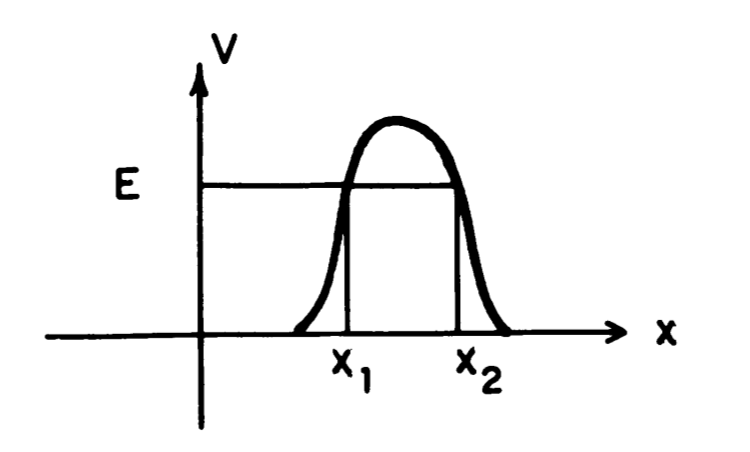
\includegraphics[width=0.6\textwidth]{instantonfig1.jpeg}
    \caption{ \label{instantonfig1}}
  \end{figure}

我们都知道这个跃迁振幅服从WKB公式
\begin{equation}
    \bigl\lvert T(E)\bigr\rvert =\exp\biggl(-\frac{1}{\hbar}\int_{x_{1}}^{x_{2}}\dif x\: \sqrt{2(V-E)}\biggr)[1+O(\hbar)] \:, \label{instanton1.7}
\end{equation}
其中$x_{1}$和$x_{2}$使得这个区域内的$V(x)$大于$E$. 
\begin{tcolorbox}
    一个非常简单的解释: 波函数可以近似写为$\exp(\mi p x/\hbar)$, 而$E=\frac{1}{2}p^{2}+V$, 所以在$E<V$时, $p=\mi\sqrt{2(V-E)}$, 波函数指数衰减.
\end{tcolorbox}
然而, 这个势垒隧穿在微扰论的任何阶都没有看到, 这是因为方程\eqref{instanton1.7}比$\hbar$的任意幂次都衰减的快, 因此也就比$g$的任意幂次都衰减得快.

在量子场论中, 尤其是量子色动力学中, 有类似于量子力学中的隧穿现象的效应, 这也就是所谓的瞬子.

{\heiti{符号说明}}: 时空特征是$({+}{-}{-}{-})$, $x^{0}$是时间坐标, $g_{\mu\nu}$是时空度规, $x^{4}=-\mi x^{0}$是到欧几里得时空的延拓.

\section{粒子力学中的瞬子和回弹} \label{instanton:sec2}

\subsection{欧几里得泛函积分} \label{instanton:sec2.1}

在本节我们继续处理单位质量的无自旋粒子在一维势下运动的理论:
\begin{equation}
    H = \frac{p^2}{2} + V(x) \:. \label{instanton2.1}
\end{equation}
这是一个量子力学问题, 但我们不采用处理这类问题的标准方法, 而是容易推广到量子场论的方法.

我们的基本工具是Feynman历史求和的欧几里得版:
\begin{equation}
    \langle x_{f} \vert \me^{-HT/\hbar} \vert x_{i}\rangle =N \int [\dif x]\, \me^{-S/\hbar} \:. \label{instanton2.2}
\end{equation}
方程\eqref{instanton2.2}左边的$\lvert x_{i}\rangle$和$\lvert x_{f}\rangle$是位置本征态, $H$是哈密顿量, 而$T$是一个正数. 利用能量本征态
\begin{equation}
    H\vert n \rangle = E_{n} \vert n\rangle \label{instanton2.3}
\end{equation}
展开方程\eqref{instanton2.2}左边, 那么就有
\begin{equation}
    \langle x_{f} \vert \me^{-HT/\hbar} \vert x_{i}\rangle 
    = \sum_{n}\me^{-E_{n}T/\hbar}  \langle x_{f} \vert n\rangle \langle n \vert x_{i}\rangle  \:. \label{instanton2.4}
\end{equation}
这个展开在大$T$时的领头项给出了能量最低的本征态的能量和波函数.

在方程\eqref{instanton2.2}右边, $N$是归一化常数, $S$是欧几里得作用量
\begin{equation}
    S=\int_{-T/2}^{T/2} \dif t\:\biggl[\frac{1}{2}\biggl(\frac{\dif x}{\dif t}\biggr)^{2}+V\biggr] \:, \label{instanton2.5}
\end{equation}
而$[\dif x]$代表对所有满足边界条件$x(-T/2)=x_{i}$和$x(T/2)=x_{f}$的函数$x(t)$积分. 更具体一些, 如果$\overline{x}$是满足边界条件的任意函数, 那么满足边界的一般函数可以写成
\begin{equation}
    x(t)=\overline{x}(t)+\sum_{n}c_{n}x_{n}(t) \:, \label{instanton2.6}
\end{equation}
其中$x_{n}$是在边界处为零的实正交函数完备集,
\begin{subequations}\label{instanton2.7}
    \begin{gather}
        \int_{-T/2}^{T/2} \dif t\: x_{n}(t)x_{m}(t) = \delta_{nm} \:, \label{instanton2.7a} \\
        x_{n}(\pm T/2)=0 \:.  \label{instanton2.7b}
    \end{gather}
\end{subequations}
这样, 测度就定义成
\begin{equation}
    [\dif x] = \prod_{n} (2\pi\hbar)^{-1/2} \dif c_{n} \:. \label{instanton2.8}
\end{equation}
(这里的归一化常数$N$依赖于测度的定义, 但是归一化常数会抵消, 所以不需要它的准确定义.)

方程\eqref{instanton2.2}右边可以用半经典(小$\hbar$)极限计算. 在这个情况下, 泛函积分由$S$的稳定点主导. 简单起见, 我们假定只有一个这样的稳定点, 我们将其记为$\overline{x}$, 它满足牛顿方程
\begin{equation}
    \frac{\delta S}{\delta x}\biggr\vert_{x=\overline{x}} = 
    -\frac{\dif^{2}\overline{x}}{\dif t^{2}} + V'(\overline{x}) = 0 \label{instanton2.9}
\end{equation} 
其中加撇号代表对$x$的导数. 更进一步, 我们令$x_{n}$是$S$在$\overline{x}$处的二阶变分导数的本征函数,
\begin{equation}
    -\frac{\dif^{2} x_{n}}{\dif t^{2}} + V''(\overline{x})x_{n} = \lambda_{n}x_{n} \:. \label{instanton2.10} 
\end{equation}
那么, 在小$\hbar$极限下, 这个积分变成高斯积分的乘积, 所以有
\begin{align}
    \langle x_{f} \vert \me^{-HT/\hbar} \vert x_{i}\rangle 
   & = N \me^{-S(\bar{x})/\hbar}\prod_{n}\lambda_{n}^{-1/2}[1+O(\hbar)] \nonumber \\
   &= N \me^{-S(\bar{x})/\hbar}\Bigl[\det\bigl(-\partial_{t}^{2}+V''(\overline{x})\bigr)\Bigr]^{-1/2}[1+O(\hbar)] \:. \label{instanton2.11}
\end{align}
如果有数个稳定点, 一般需要求和.
\begin{tcolorbox}
    这里解释一下方程\eqref{instanton2.10}和\eqref{instanton2.11}, 在$\overline{x}$附近展开$S$, 并设微扰为$\eta$, 那么
    \begin{align*}
        \delta S&= S(\overline{x}+\eta)-S(\overline{x}) 
        = \int \dif t\, \Bigl(\tfrac{1}{2}\bigl(\dot{\overline{x}}+\dot{\eta}\bigr)^{2}+V(\overline{x}+\eta)-\tfrac{1}{2}\dot{\overline{x}}^{2}-V(\overline{x})\Bigr) \\
        &=\int \dif t\,\Bigl(\dot{\overline{x}}\dot{\eta}- V'(\overline{x})\eta+\tfrac{1}{2}\dot{\eta}^{2}+\tfrac{1}{2}V''(\overline{x})\eta^{2}+O(\eta^{2})\Bigr)
        =\frac{1}{2}\int \dif t\, \eta(-\partial_{t}^{2}+V'')\eta
    \end{align*}
在最后一个等号这里使用了牛顿方程\eqref{instanton2.9}, 分部积分并忽略了$\eta$的高阶项. 

用$(-\partial_{t}^{2}+V'')$的本征函数完备集$\{x_{n}\}$展开$\eta=\sum c_{n}x_{n}$, 利用方程\eqref{instanton2.7}就得到了
\begin{equation*}
    \delta S= \frac{1}{2} \lambda_{n}c_{n}^{2}
\end{equation*}
那么
\begin{align*}
    N \int [\dif x]\, \me^{-S/\hbar}&=N \me^{-S(\overline{x})/\hbar} \int [\dif x]\, \me^{-\delta S/\hbar} \\
    &=N \me^{-S(\overline{x})/\hbar} \int \prod_{n} (2\pi\hbar)^{-1/2} \dif c_{n}\:\me^{-\frac{1}{2} \lambda_{n}c_{n}^{2}/\hbar}
    =N \me^{-S(\overline{x})/\hbar}\prod_{n} \lambda_{n}^{-1/2} .
\end{align*}
\end{tcolorbox}

根据方程\eqref{instanton2.9}, 能量是
\begin{equation}
    E=\frac{1}{2}\biggl(\frac{\dif\overline{x}}{\dif t}\biggr)^{2} - V(\overline{x})
\end{equation}
这可以用来决定方程\eqref{instanton2.9}的解的定性性质.

\begin{figure}[h]
    \centering
    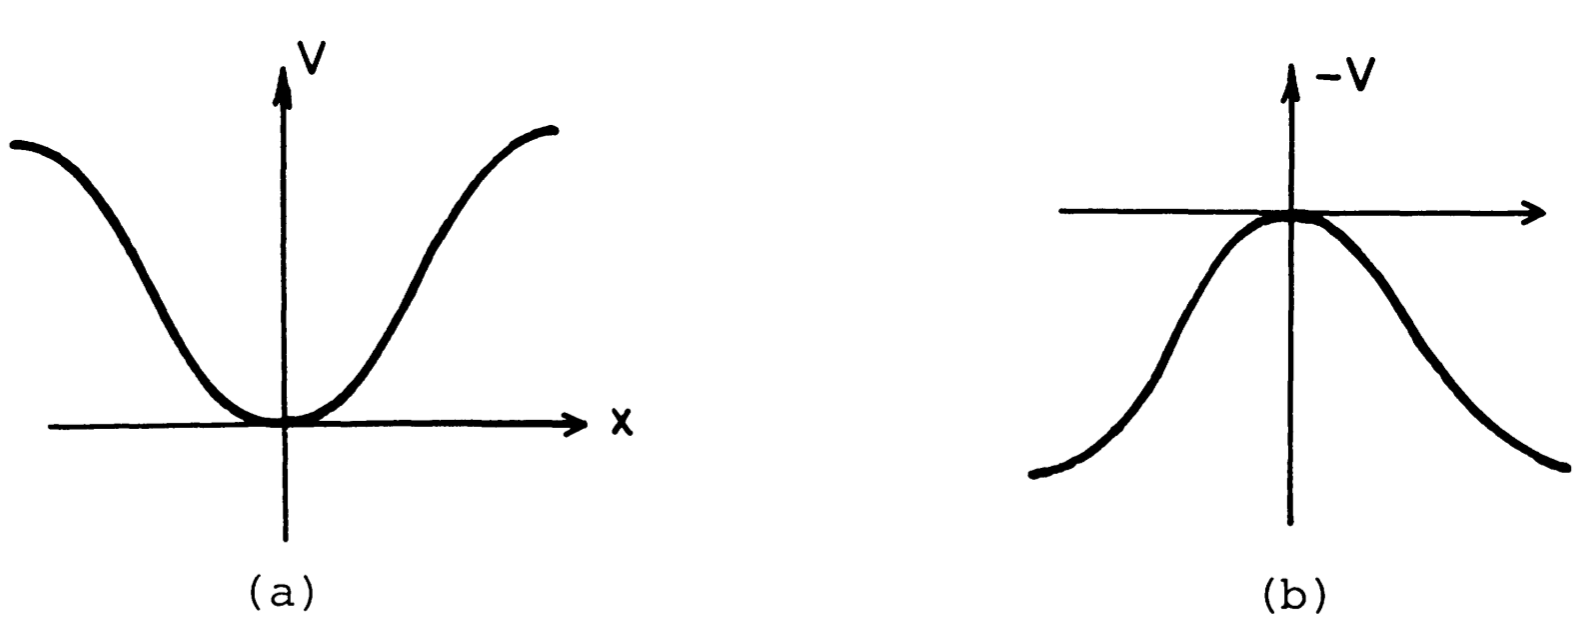
\includegraphics[width=0.8\textwidth]{instantonfig2.jpeg}
    \caption{ \label{instantonfig2}}
  \end{figure}
作为一个简单例子, 考虑图\ref{instantonfig2}(a)中的势能. 选择$x_{i}=x_{f}=0$. 方程\eqref{instanton2.9}满足边界条件的解显然是
\begin{equation}
    \overline{x}=0 . \label{instanton2.13}
\end{equation}
对于这个解, $S(\overline{x})=0$. 那么, 从方程\eqref{instanton2.11}
\begin{equation}
    \langle 0 \vert \me^{-HT/\hbar} \vert 0\rangle = 
    N[\det(-\partial_{t}^{2}+\omega^{2})]^{-1/2}[1+O(h)] \:, \label{instanton2.14}
\end{equation}
其中
\begin{equation}
    \omega^{2}=V''(0) \:. \label{instanton2.15}
\end{equation}

可以证明, 对于很大的$T$,
\begin{equation}
    N[\det(-\partial_{t}^{2}+\omega^{2})]^{-1/2} \simeq \biggl(\frac{\omega}{\pi\hbar}\biggr)^{1/2}\me^{-\omega T/2}.  \label{instanton2.16}
\end{equation}
根据方程\eqref{instanton2.4}, 基态能量是
\begin{equation}
    E_{0}=\frac{1}{2}\omega\hbar[1+O(\hbar)] \:. \label{instanton2.17}
\end{equation}
同理, 基态粒子处在原点的几率是
\begin{equation}
     \bigl\lvert \langle x{=}0 \vert n{=}0 \rangle \bigr\rvert^{2} =
     (\omega/\pi\hbar)^{1/2}[1+O(\hbar)] .
\end{equation}

这些当然是正确的半经典结果. 在小$\hbar$极限下, 粒子处在位于原点的谐振子基态中, 能量就是谐振子的基态能量.

\begin{tcolorbox}[breakable]
    推导方程\eqref{instanton2.16}的两种方法:

    (1)蛮干法(Poor man's way): 求解如下微分方程
\[
 (-\partial_{t}^{2}+\omega^{2})f= \lambda_{n}f
\]
由于$f$要满足边界条件$f(\pm T/2)=0$, 所以$\lambda_{n}>\omega^{2}$, 并要满足
\[
 \sqrt{\lambda_{n}-\omega^{2}} = \frac{n\pi}{T}    
\]
那么根据方程\eqref{instanton2.11}, 
\begin{align*}
    [\det(-\partial_{t}^{2}+\omega^{2})]^{-1/2}
    =\prod_{n}\biggl(\frac{n^{2}\pi^{2}}{T^{2}}+\omega^{2}\biggr)^{-1/2}
\end{align*}
上式需要重整化, 除以一个不依赖于$\omega$的无限大常数$[\det(-\partial_{t}^{2})]^{-1/2}$, 得到
\begin{align*}
    [\det(-\partial_{t}^{2}+\omega^{2})]^{-1/2}&=\prod_{n}\Biggl(
        1+ \biggl(\frac{\omega T}{n\pi}\biggr)^{2}\Biggr)^{-1/2} \\
        &= \biggl(\frac{\sinh(\omega T)}{\omega T}\biggr)^{-1/2}
\end{align*}
在$T$很大时, $\sinh(\omega T)\simeq \me^{\omega T}$. 常数$N$可以通过考虑自由粒子来决定, 这里不再赘述.

(2) Coleman的方法, 根据定义
\[
\det(-\partial_{t}^{2}+W)=\prod_{n}\lambda_{n}    
\]
其中$\lambda_{n}$是算符$(-\partial_{t}^{2}+W)$的本征值, 那么$(-\partial_{t}^{2}+W-\lambda)$的本征值是$\lambda_{n}-\lambda$. 这样就有
\[
\frac{\det(-\partial_{t}^{2}+W^{(1)}-\lambda)}{\det(-\partial_{t}^{2}+W^{(2)}-\lambda)}  = \frac{\psi_{\lambda}^{(1)}(T/2)}{\psi_{\lambda}^{(2)}(T/2)}  .
\]
这里$\psi$满足
$(-\partial_{t}^{2}+W^{(i)})\psi_{\lambda}^{(i)}=\lambda \psi_{\lambda}^{(i)}$以及边界条件$\psi_{\lambda}(-T/2)=0$和$\dot{\psi}_{\lambda}(-T/2)=1$. 显然$\psi_{\lambda}^{(i)}$只有$\lambda=\lambda_{n}$时满足边界条件$\psi_{\lambda}^{(i)}(\pm T/2)=0$. 将上式左右两边视为$\lambda$的函数, 那么左右两边就有相同的零点和极点, 所以相等.

由此可得
\[
    \frac{\det(-\partial_{t}^{2}+W)}{\psi_{0}(T/2)} =\text{常数} = \pi\hbar N^{2} 
\]
其中$N$是一个常数. (这也是Coleman对$N$的定义.) 对于$W=\omega^{2}$, 可以解出
\[
\psi_{0}=\omega^{-1} \sinh \omega(t+T/2)\:,   
\]
进而也就得到了方程\eqref{instanton2.16}

\end{tcolorbox}


\subsection{双井与瞬子} \label{instanton:sec2.2}

我们现在转向不那么平庸的问题, 图\ref{instantonfig3}(a)所示的双井. 假定势是偶函数, $V(x)=V(-x)$, 它的最小值点记为$\pm a$. 选择一个常数, 使得$V$的最小值是0, 并将$V''(\pm a)$记为$\omega^{2}$.
\begin{figure}[h]
    \centering
    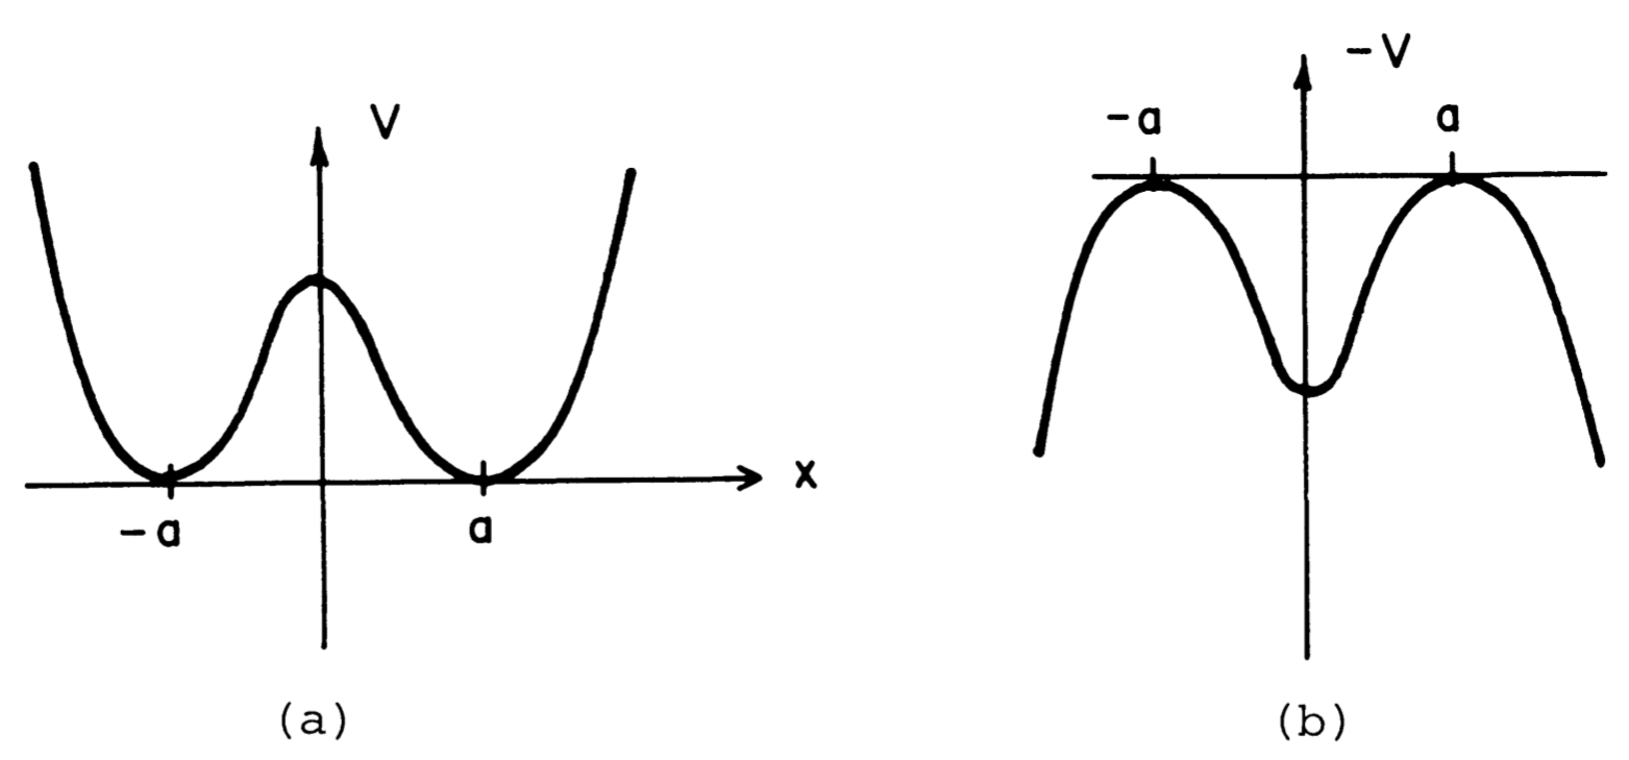
\includegraphics[width=0.8\textwidth]{instantonfig3.pdf}
    \caption{ \label{instantonfig3}}
\end{figure}

我们将尝试计算
\begin{subequations}
    \begin{align}
        \langle {-}a \vert \me^{-HT} \vert {-}a \rangle &= \langle a \vert \me^{-HT} \vert a \rangle \:, \label{instanton2.19a}\\ 
        \langle a \vert \me^{-HT} \vert {-}a \rangle &= \langle {-}a \vert \me^{-HT} \vert a \rangle \:,\label{instanton2.19b}
    \end{align}
\end{subequations}
方法是通过半经典极限方程\eqref{instanton2.11}来近似泛函积分. 和前面一样, 先求解与边界条件相容的经典欧几里得运动方程, \eqref{instanton2.9}. 

当然, 两个这样的解是粒子待在两个井底(或者说图\ref{instantonfig3}(b)的两个山顶). 然而还有另一种有趣的解, 在$-T/2$时待在其中一个山顶, 然后在$T/2$时跑到另一个山顶.
由于我们最后会把$T$取为无穷大, 我们将专注于这个极限下的解形式, 即粒子在无穷远的过去从一个山顶离开, 然后在无穷远的未来达到另一个山顶. 在这个情况下, 运动方程的解的能量为零; 
所以
\begin{equation}
    \dif x/\dif t =\sqrt{2V}. \label{instanton2.20}
\end{equation}
等效地有
\begin{equation}
    t= t_{1}+\int_{0}^{x}\dif x' \: (2V)^{-1/2} \:, \label{instanton2.21}
\end{equation}
其中$t_{1}$是积分常数, $x(t_{1})$为零.

\begin{figure}[h]
    \centering
    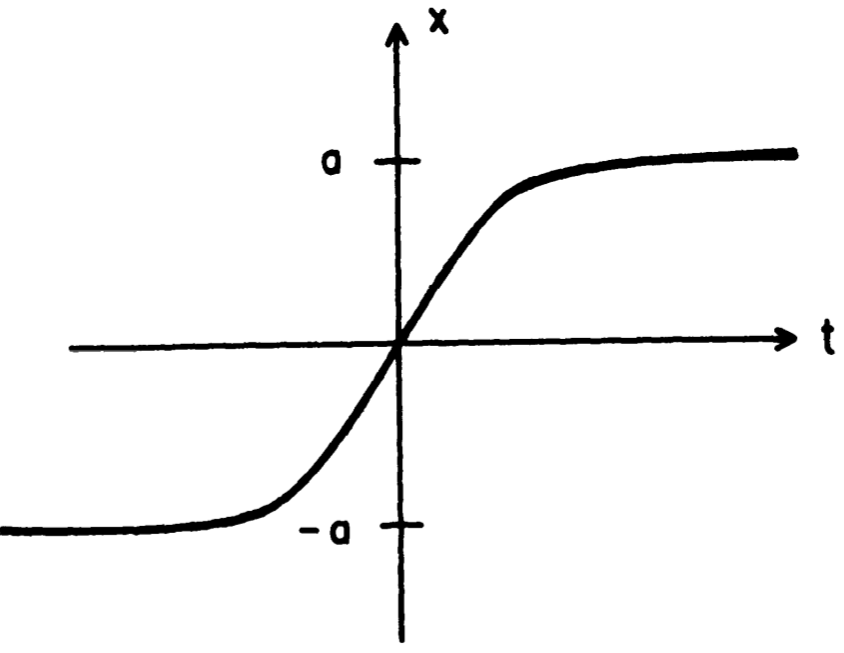
\includegraphics[width=0.5\textwidth]{instantonfig4.jpeg}
    \caption{ \label{instantonfig4}}
  \end{figure}

解的图示参看图\ref{instantonfig4}; 它被称为``中心在$t_{1}$的瞬子''. 瞬子这一词汇是't Hooft发明的. 灵感来源于它们的数学结构十分类似于所谓的孤子(solitons)或鼓包(lump), 
经典场论的类粒子解: 因此称为``-子''. 然而, 不像鼓包, 它们在时间(尽管是欧几里得时间)中是局域的: 因此是``瞬-''. 由于相同的原因, Polyakov称其为``赝粒子(pseudoparticle)'', 也见于文献.

当然, 我们可以也可以构建从$a$到${-}a$的解, 将方程\eqref{instanton2.21}中的$t$换为$-t$即可; 它们被称为``反瞬子''.

这些解有两个很重要的性质:
\begin{enumerate}
    \item 从方程\eqref{instanton2.20}可以导出瞬子(或反瞬子)作用量的一个简单表达式
    \begin{equation}
        S_{0}=\int \dif t\:\bigl[\tfrac{1}{2}\dot{x}^{2}+V\bigr] =\int \dif t \: \dot{x}^{2} = \int_{-a}^{a}\dif x\:\sqrt{2V} \:. \label{instanton2.22}
    \end{equation}
    注意这与势垒隧穿公式\eqref{instanton1.7}中出现的积分相同. 我们会在后面看到这不是个巧合.
    \item 对于大$t$, $x$趋于$a$, 方程\eqref{instanton2.20}可以近似为
    \begin{equation}
        \dot{x} = \omega(a-x) \:. \label{instanton2.23}
    \end{equation}
    因此, 对于大$t$,
    \begin{equation}
        (a-x) \propto \me^{-\omega t} \:. \label{instanton2.24}
    \end{equation}
    因此瞬子是一个非常定域的物体, 它的尺寸大约是$1/\omega$阶的.
\end{enumerate}

这是十分重要的, 因为这意味着: 当$T$很大时, 瞬子和反瞬子不仅是运动方程的近似解; 相距甚远的瞬子和反瞬子串联而成的场构型也是近似解. 

泛函积分将通过对所有这样的构型求和计算, 其中每个构型有$n$个物体(瞬子或反瞬子), 中心处在$t_{1},\ldots,t_{n}$, 其中
\begin{equation}
    T/2>t_{1}>\cdots>t_{n}>-T/2\:. \label{instanton2.25}
\end{equation}

图\ref{instantonfig5}展示了这样一个构型. $T$相比于瞬子尺寸要大很多; 因此图\ref{instantonfig4}的光滑曲线在图5的尺度上就变成了尖锐的跃变. 

\begin{figure}[h]
    \centering
    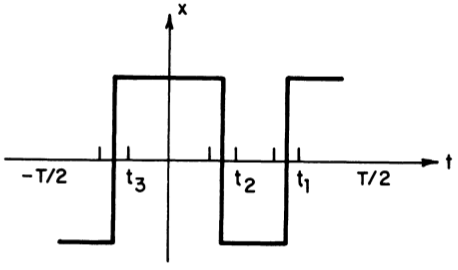
\includegraphics[width=0.6\textwidth]{instantonfig5.jpeg}
    \caption{ \label{instantonfig5}}
  \end{figure}

现在是计算:
\begin{enumerate}
    \item 对于$n$个相距甚远的物体, $S$就是$n S_{0}$. 要考虑到作用量在指数上.
    \item 泛函行列式的计算需要一些技巧. 我们把时间演化算符$\me^{-HT}$视为图\ref{instantonfig5}中时间轴上垂直线所标出的点之间的演化算符的乘积. 
    要不是存在含有瞬子和反瞬子的小区间, $V''$在整个时间上等于$\omega^{2}$, 因此我们所获得的结果与\ref{instanton:sec2.1}节中的单井势的结果相同, 
    \begin{equation}
        \biggl(\frac{\omega}{\pi\hbar}\biggr)^{1/2} \me^{-\omega T/2} \:. \label{instanton2.26}
    \end{equation}
    含有瞬子和反瞬子的小区间修正了这个公式. 因此我们得到
    \begin{equation}
        \biggl(\frac{\omega}{\pi\hbar}\biggr)^{1/2} \me^{-\omega T/2}K^{n} \:. \label{instanton2.27}
    \end{equation}
    其中$K$可以通过计算只有一个瞬子的情况得到.
    \item 我们必须要对瞬子中心所处的位置的积分:
    \begin{equation}
        \int_{-T/2}^{T/2} \dif t_{1}\int_{-T/2}^{t_{1}} \dif t_{2} \cdots \int_{-T/2}^{t_{n-1}} \dif t_{n} 
        =T^{n}/n! \:. \label{instaton2.28}
    \end{equation}
    \item 我们无法自由地分配瞬子和反瞬子. 例如, 如果我们从${-}a$出发, 那么第一个遇到的物体必然是瞬子, 下一个必然是反瞬子, 以此类推. 
    更进一步, 如果我们最后返回${-}a$, $n$必须是偶数. 同样, 如果我们最后停到了$a$, $n$必须是奇数. 
\end{enumerate}

因此,
\begin{equation}
    \langle{-}a\vert \me^{-HT/\hbar} \vert {-a}\rangle 
    =\biggl(\frac{\omega}{\pi\hbar}\biggr)^{1/2} \me^{-\omega T/2} 
    \sum_{\text{even }n} \frac{\bigl(K\me^{-S_{0}/\hbar}T\bigr)^{n}}{n!}[1+O(\hbar)] \:, \label{instanton2.29}
\end{equation}
而$\langle a\vert \me^{-HT/\hbar} \vert {-a}\rangle $由只对奇数$n$求和的相同表达式给出. 这些求和是平庸的:
\begin{equation}
    \langle \pm a\vert \me^{-HT/\hbar} \vert {-a}\rangle 
    =\frac{1}{2}\biggl(\frac{\omega}{\pi\hbar}\biggr)^{1/2} \me^{-\omega T/2}
    \Bigl[\exp\bigl(K\me^{-S_{0}/\hbar}T\bigr)\pm \exp\bigl(-K\me^{-S_{0}/\hbar}T\bigr)\Bigr] 
    \:, \label{instanton2.30}
\end{equation}
(从现在起将省略因子$[1+O(\hbar)]$.)

与方程\eqref{instanton2.4}比较, 我们现在有两种能量最底态, 其能量是
\begin{equation}
    E_{\pm} = \tfrac{1}{2}\hbar\omega \pm \hbar K \me^{-S_{0}/\hbar} \:. \label{instanton2.31}
\end{equation}
如果我们把这些本征态记为$\lvert + \rangle$和$\lvert - \rangle$, 我们看到
\begin{equation}
    \bigl \lvert \langle + \vert {\pm} a \rangle \bigr \rvert^{2} = \bigl \lvert \langle - \vert {\pm} a \rangle \bigr \rvert^{2} 
    =\langle a\vert -\rangle \langle - \vert {-}a\rangle =-\langle a\vert +\rangle \langle + \vert {-}a\rangle 
    =\frac{1}{2} \biggl(\frac{\omega}{\pi\hbar}\biggr)^{1/2} \:. \label{instanton2.32}
\end{equation}
当然, 它们是预期的结果: 能量本征态是中心在两个井底的谐振子态在空间上为偶或为奇的组合; 两个能量本征态的简并只被势垒隧穿破坏了(因此能量差正比于势垒隧穿因子$\me^{-S_{0}/\hbar}$), 而能量较低的态, 即我们记为$\lvert -\rangle$的那个, 在空间上为偶的组合. \\
\begin{remark}
设$\vert + \rangle= (m_{+}\lvert 0_{+}\rangle+n_{+}\lvert 0_{-}\rangle)/\sqrt{2}$和$\vert - \rangle= (m_{-}\lvert 0_{+}\rangle+n_{-}\lvert 0_{-}\rangle)/\sqrt{2}$, 其中$\lvert 0_{\pm}\rangle$是中心分别处在$\pm a$的谐振子态. 方程\eqref{instanton2.32}给出$m_{+}=-n_{+}$和$m_{-}=n_{-}$, 以及它们的范数为1.
\end{remark}

下个任务是计算$K$. 在计算之前, 我们先对所做的事情做一些评论:
\begin{enumerate}
    \item 实际上我们没有权利在方程\eqref{instanton2.31}中保留第二项. 不仅是因为它指数式小于第一项, 它也指数式得小于对第一项的未知$O(\hbar^{2})$修正. 然而这是对能量差$E_{+}-E_{-}$的领头阶修正; 一个更加严格的做法是仅在能量差的表达式中保留这一项, 而在单个能量的表达式中略去它.
    \item 我们的近似基于瞬子和反瞬子相距甚远的假定. 作为一个自洽性检验, 我们应该验证最后结果的主要部分来自于这样的构型. 
    
    这个检验很容易做. 对于固定的$x$, 指数系数$\sum x^{n}/n!$中的项随着$n$的增长而增长直到$n$到达$x$的量级, 在这之后, 开始快速衰减. 对方程\eqref{instanton2.29}中的求和应用这个性质, 我们看到重要的项是那些
    \begin{equation}
        n \lesssim KT \me^{-S_{0}/\hbar} \label{instanton2.33}
    \end{equation}
    的项. 这就是说, 对于小$\hbar$, 求和中重要的项是那些瞬子和反瞬子密度$n/T$是指数量级小数的项, 因此平均间隔非常大. 注意到这个平均间隔$K\me^{-S_{0}\hbar}$实际上独立于$T$; 我们的近似实际上是小$\hbar$近似; 只要$T$足够大, 这个条件就独立于$T$而成立.

    瞬子相距甚远这个近似被称为稀薄气体近似.
    \item 最后进一步解释下$S$的近似稳相点这个概念. 我们先来看单变量积分,
    \begin{equation}
        I=\int_{0}^{T} \dif t\: \me^{-S(t)/\hbar} \:, \label{instanton2.34}
    \end{equation}
    其中$S$是$t$的单调递减函数, 它的渐进值是$S(\infty)$. 因此这个被积函数在积分区域中没有稳相点. 然而对于小$\hbar$和大$T$, 很容易找到这个积分的如下近似形式
    \begin{equation}
        I\approx T \me^{-S(\infty)/\hbar} \:. \label{instanton2.35}
    \end{equation}
    大概地讲, 这个积分被无穷远处的稳相点所主导. 将这个现象推广到多维积分是直接的: 我们假定被积函数的图像有某种波谷; 沿着谷底的线会随着我们趋于无穷远而变平. 换言之, 在高维空间中有一条线, 使得被积函数在垂直于线的方向上在该线所处的位置达到最小值, 并在沿着这条线趋于无穷远时达到某个近似值. 当然这个线本身可以推广至超平面. ``近似稳相点''实际上就是这样的情况; 瞬子和反瞬子的所在就是沿着谷底的变量; $S$仅在它们趋于无穷远处变得稳定(并等于$nS_{0}$).
\end{enumerate}
\vspace{0.5cm}
现在我们来计算$K$.

我们现在必须要研究本征方程\eqref{instanton2.10}, 其中$\overline{x}$是单瞬子. 由于时间平移不变性, 这个方程必然有一个本征值为零的本征函数,
\begin{equation}
    x_{1} = S_{0}^{-1/2} \dif \overline{x}/\dif t \:. \label{instanton2.36}
\end{equation}
(归一化因子来自于方程\eqref{instanton2.22}.)
\begin{tcolorbox}
    我们稍微解释一下函数\eqref{instanton2.36}的来源. 这里的时间平移性是指: 当时间$T$是无穷时, 无论单瞬子$\overline{x}$的中心在哪, 作用量$S(\bar{x})$都是相同的. 设中心在$t_{1}$的单瞬子为$\bar{x}(t-t_{1})$, 那么对于两个相距很近的单瞬子, 我们就有
    \begin{equation*}
        0=\delta S= S[\overline{x}(t-t_{1}-\Delta t_{1})]-S[\overline{x}(t-t_{1})]=\frac{1}{2}\int \dif t\, \eta(-\partial_{t}^{2}+V'')\eta
    \end{equation*} 
    其中$\eta=\overline{x}(t-t_{1}-\Delta t_{1})-\overline{x}(t-t_{1})=-\Delta t_{1} \, \dot{\overline{x}}(t-t_{1})$. 由于算符$(-\partial_{t}^{2}+V'')$没有非负本征值, 所以这个$\eta$肯定是这个算符本征值为零的本征函数. 归一化因子是要求
    \begin{equation*}
        \int \dif t\: x_{1}^{2} =1 
    \end{equation*}
    得到的, 其中用到了方程\eqref{instanton2.22}.
\end{tcolorbox}
如果我们要想对方程\eqref{instanton2.6}中的相应展开系数$c_{1}$积分, 我们会遇到无穷大, 但这个积分实际上已经在对瞬子中心的积分\eqref{instaton2.28}中做过了. 
原因是, 瞬子$\overline{x}(t)$的中心移动所产生的微扰是:
\begin{equation}
    \eta =\dot{\overline{x}} \Delta t_{1} \:. \label{instanton2.37}
\end{equation}
而这造成了本征函数展开系数的扰动
\begin{equation}
    \eta =x_{1}\Delta c_{1} \:. \label{instanton2.38}
\end{equation}
因此,
\begin{equation}
    (2\pi\hbar)^{-1/2} \dif c_{1} = (S_{0}/2\pi\hbar)^{1/2} \dif t_{1} \:.
\end{equation}

因此, 在计算泛函行列式时, 我们应该排除零本征值, 但我们应该该$K$引入因子$(S_{0}/2\pi\hbar)^{1/2}$. 因此, 单瞬子对这个跃迁元的贡献是
\begin{equation}
    \langle a \vert \me^{-HT} \vert {-}a\rangle _{\text{one inst.}} =N T  (S_{0}/2\pi\hbar)^{1/2} \me^{-S_{0}/\hbar}
    \bigl(\det\nolimits'[-\partial_{t}^{2}+V''(\overline{x})]\bigr)^{-1/2} \:, \label{instanton2.40}
\end{equation}
其中$\det'$是指在计算行列式时已经排除了零本征值. 与\eqref{instanton2.29}相比较, 我们得到
\begin{equation}
    K= (S_{0}/2\pi\hbar)^{1/2} \Biggl\lvert \frac{\det(-\partial_{t}^{2}+\omega^{2})}{\det'\bigl(-\partial_{t}^{2}+V''(\overline{x})\bigr)} \Biggr\rvert^{1/2} \:.
\end{equation}

一些注解:
\begin{enumerate}
    \item 为了真的把所有元素缝合在一起, 我们应该证明我们所得到的能级分裂公式与通过传统波动力学方法得到的相同. 这个会在附录中解释.
    \item 我们现在来论述算符$-\partial_{t}^{2}+V''(\overline{x})$的本征值都是非负的. 这个算符是Schr\"{o}dinger方程中的算符, 本征值越大的本征函数拥有更多的节点(零点), 或者更多的波峰波谷(这样本征函数的频率也就越高). 瞬子是单调增函数, 它的导数没有节点, 再加上这个导数是这个算符本征值为零的本征函数. 证毕.
    \item $K$正比于$\hbar^{-1/2}$. 这个因子来自于时间平移不变性产生的零模. 稍后我们会分析拥有更大对称群的理论, 对于这些理论, 瞬子有多个这样的零模. 显然, 每个零模都会给一个$\hbar^{-1/2}$因子. 这种对$\hbar$的幂次计数的规则将起到重要作用, 正如第\ref{instanton:sec1}节所解释的那样, 对$\hbar$的幂次计算等同于对耦合常数的幂次计数.
\end{enumerate}

\subsection{周期势}

我们来考虑如图\ref{instantonfig6}(a)所示的周期势. (方便起见, $V$的最小值点被取成了整数.) 如果忽略势垒隧穿, 能量本征态就是无限多个简并态, 每个都集中在某个井底. 
势垒隧穿将单个本征值变成了连续的本征值带; 真正的能量本征态势单位平移的本征态, Bloch波. 我们现在看一下如何用瞬子方法推导这个旧结果.
\begin{figure}[h]
    \centering
    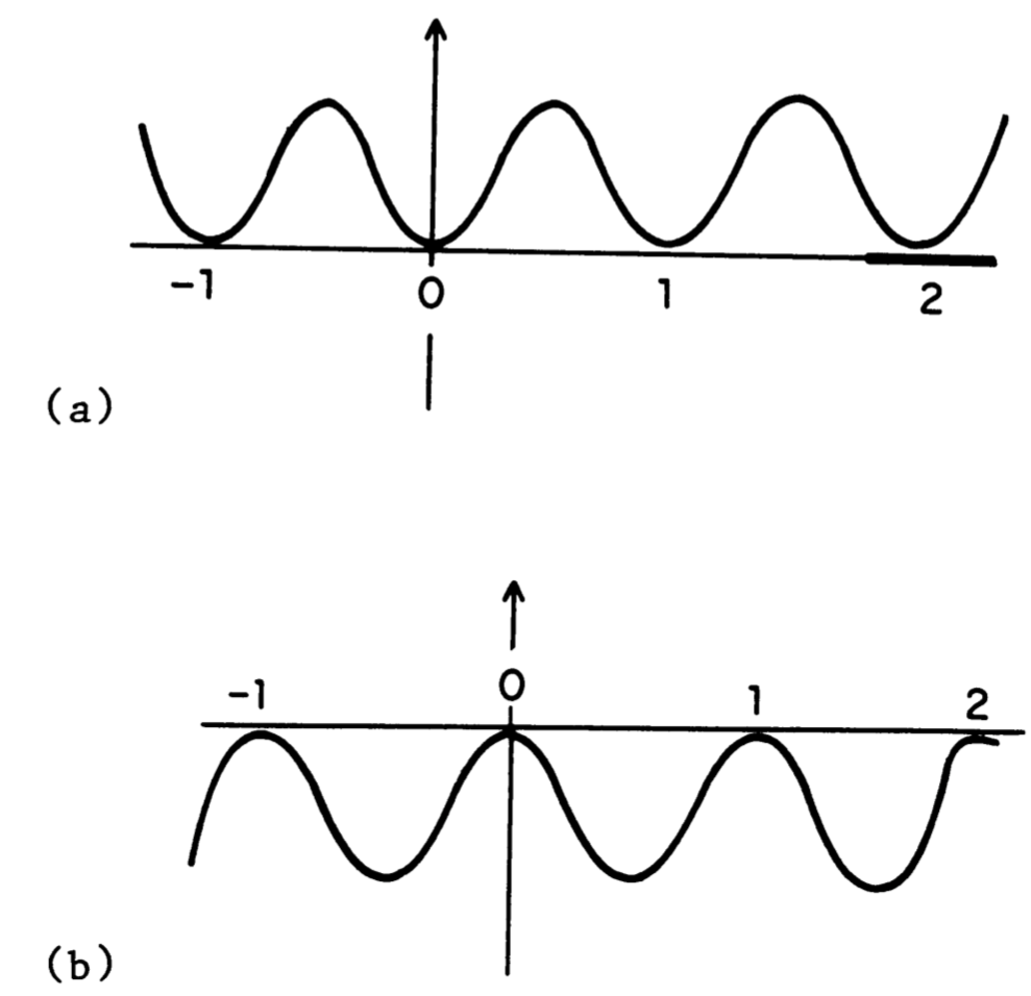
\includegraphics[width=0.5\textwidth]{instantonfig6.pdf}
    \caption{ \label{instantonfig6}}
  \end{figure}

我们从图\ref{instantonfig6}(b)中可以看到, 这里的瞬子和前面的很像. 唯一新的地方是瞬子现在可以从任何初始位置$x=j$出发, 然后去往下一个$x=j+1$. 反瞬子则是从$x=j$到$x=j-1$. 
其余的和之前相同.

因此, 当做稀薄气体求和时, 我们可以在实轴上分布瞬子和反瞬子, 不再有瞬子和反瞬子交替分布这样的约束. 当然, 当我们沿着线行进时, 
每个瞬子或反瞬子都必须从它的前任者的终点出发. 更进一步, 瞬子的总数减去反瞬子的总数必须等于初始位置本征态和终末位置本征态的$x$的变化.

因此我们得到
\begin{equation}
    \langle j_{+} \vert \me^{-HT/\hbar} \vert j_{-} \rangle = \biggl( \frac{\omega}{\pi\hbar}\biggr)^{1/2} \me^{-\omega T/2}
    \sum_{n=0}^{\infty}\sum_{\overline{n}=0}^{\infty} \frac{1}{n!\overline{n}!} \Bigl( K\me^{-S_{0}/\hbar}T\Bigr)^{n+\overline{n}}
    \delta_{n-\overline{n}\,,\,j_{+}-j_{-}} \label{instanton2.42}
\end{equation}
其中$n$是瞬子总数而$\overline{n}$是反瞬子总数. 如果我们使用恒等式
\begin{equation}
    \delta_{a,b}= \int_{0}^{2\pi} \frac{\dif \theta}{2\pi} \:\me^{\mi\theta(a-b)} \:, \label{instanton2.43}
\end{equation}
求和就变成了两个独立的指数级数, 我们发现
\begin{equation}
    \langle j_{+} \vert \me^{-HT/\hbar} \vert j_{-} \rangle = \biggl( \frac{\omega}{\pi\hbar}\biggr)^{1/2} \me^{-\omega T/2}
    \int_{0}^{2\pi}  \frac{\dif \theta}{2\pi} \:\me^{\mi\theta(a-b)}\exp\Bigl[2KT\cos\theta \me^{-S_{0}/\hbar}\Bigr] \:. \label{instanton2.44}
\end{equation}

因此我们得到了用角度$\theta$标记的连续能量本征态. 能量本征值是
\begin{equation}
    E(\theta) = \tfrac{1}{2}h\omega +2 hK \cos\theta \me^{-S_{0}/\hbar} \:. \label{instanton2.45}
\end{equation}
以及
\begin{equation}
    \langle \theta \vert j\rangle =\biggl( \frac{\omega}{4\pi^{3}\hbar}\biggr)^{1/4}  \me^{\mi j\theta} \:. \label{instanton2.46}
\end{equation}
这正是正确结果.

\subsection{非稳态与回弹}

\subsubsection*{伽利略戏仿\footnote{这里仿照了伽利略著作《关于托勒密和哥白尼两大世界体系的对话》的对话体形式, 本节中出现的沙格列陀(Sagredo)和萨尔维阿蒂(Salviati)正是此书中参与对话的两个主要人物, 名字取自伽利略的好友.}} 

\begin{figure}[h]
    \centering
    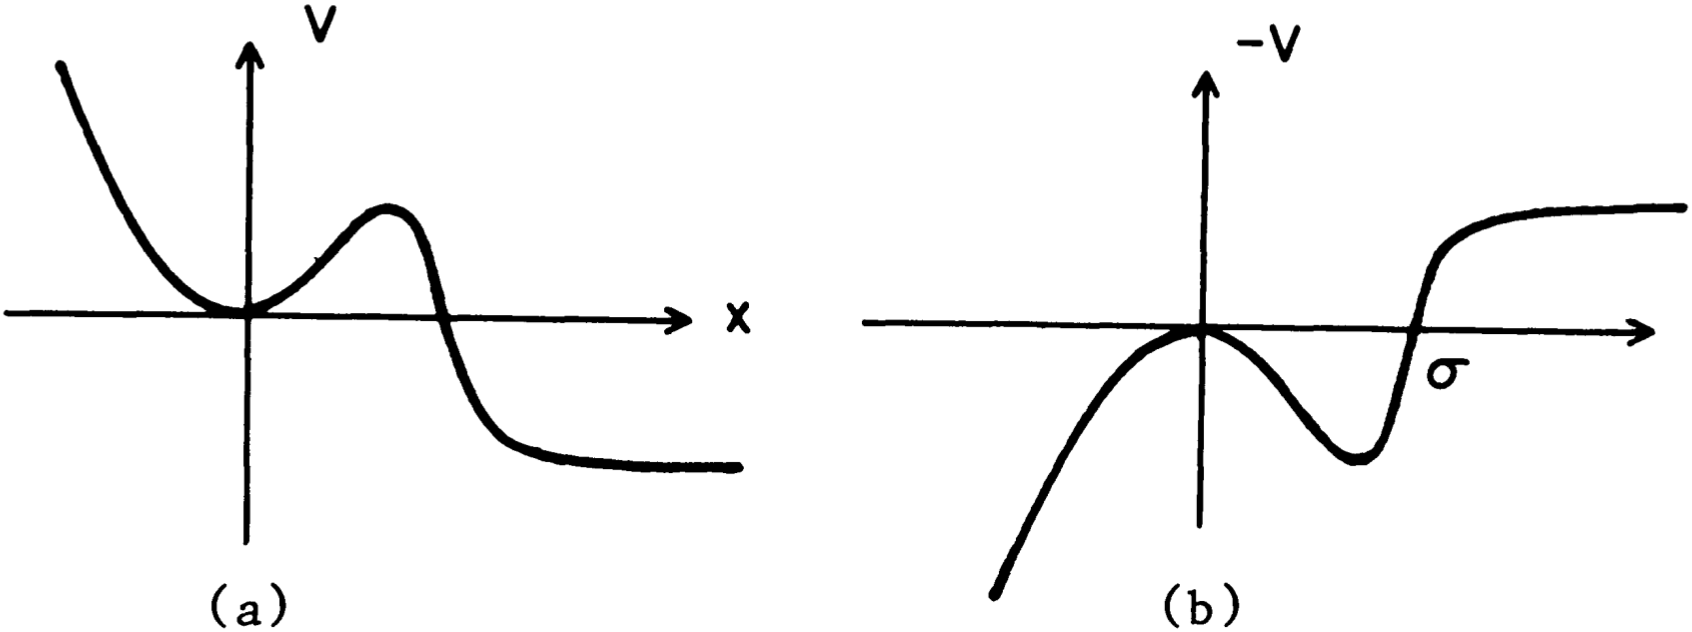
\includegraphics[width=0.7\textwidth]{instantonfig7.png}
    \caption{ \label{instantonfig7}}
  \end{figure}

\noindent {\kaishu{沙格列陀}}: 我想通过用瞬子方法研究图\ref{instantonfig7}(a)中的势以检查我对它们的理解. 如果我忽略势垒隧穿, 在半经典极限下, 这个势有一个处在井底的能量本征态. 我想计算势垒隧穿对这个态的能量的修正. 如果我把这个势上下颠倒(图\ref{instantonfig7}(b)), 我观察到经典运动方程有这样一个解: 粒子从$x=0$处的山顶出发,然后在经典转折点$\sigma$处反弹, 最后回到山顶(图\ref{instantonfig8}). 我们称这种运动为``回弹''(the bounce). 就像在研究双井势时对瞬子和反瞬子求和, 我将通过对相距甚远的回弹构型求和来计算$x=0$和$x=0$之间的跃迁矩阵元. 诚然, 除了对回弹的数目是奇是偶没有限制, 这个求和与双井势的情况相同(这里如何定义$S_{0}$、$\omega^{2}$等是显然的). 因此这里的指数级数是完整的, 而不是只有奇数项或偶数项, 这样就有
\begin{equation}
    \langle 0 \vert \me^{-HT/\hbar} \vert 0 \rangle =\biggl(\frac{\omega}{\pi\hbar}\biggr)^{1/2} \me^{-\omega T/2}
    \exp\bigl[KT \me^{-S_{0}/\hbar}\bigr] \:, \label{instanton2.47}
\end{equation}
而能量本征态是
\begin{equation}
    E_{0}=\tfrac{1}{2}\hbar\omega+\hbar K\me^{-S_{0}/\hbar} \:. \label{instanton2.48}
\end{equation}

\begin{figure}[h]
    \centering
    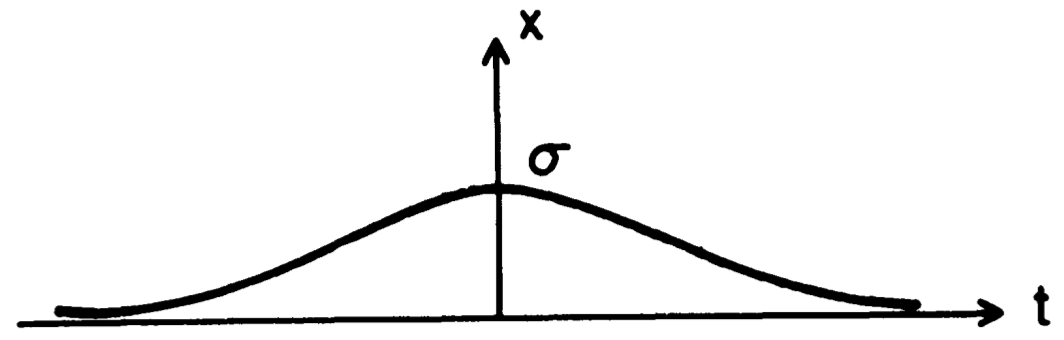
\includegraphics[width=0.5\textwidth]{instantonfig8.png}
    \caption{ \label{instantonfig8}}
  \end{figure}

\noindent {\kaishu{萨尔维阿蒂}}: 唉, 沙格列陀, 我恐怕你在三个地方出错了. 首先, 你所计算的项要远小于$\hbar^{2}$阶的项, 而你在计算过程中忽略了这样的项, 因此你没有理由保留它. 其次, 通过你的概述, 我看到这个回弹有个极大值; 而本征函数$x_{1}$正比于回弹的时间导数, 所以有一个节点. 因此它不是本征值最低的本征函数, 并且必然有一个本征值很低的无节点本征函数$x_{0}$, 这就是说, 必然有一个负本征值. $K$反比与本征值平方根之积, 因此是纯虚的. 最后, 你所研究的态由于势垒隧穿而变得不稳定, 因此你尝试计算的本征值不在哈密顿量的频谱中.

\noindent {\kaishu{沙格列陀}}: 你所说的都是正确的, 但我觉得你的批评也恰好指出了如何修正这个计算. 非稳态的能量有一个虚部; 因此只能期待$K$应该是纯虚的. 更进一步, 尽管我所计算的项相比于$E_{0}$的实部是可忽视的项, 但它是$E_{0}$虚部的领头贡献. 因此, 方程\eqref{instanton2.48}的修正版是
\begin{equation}
    \operatorname{Im}E_{0}= \Gamma/2= \hbar \lvert K \rvert \me^{-S_{0}/\hbar} \:, \label{instanton2.49}
\end{equation}
其中, 和通常一样, $\Gamma$是非稳态的展宽.

正如你所看到的, 这两个托斯卡纳人像往常一样机智敏捷, 然而他们的论证(也像往常一样)有点马虎. 沙格列陀丢了一个因子$\tfrac{1}{2}$; 正确的答案是
\begin{equation}
    \Gamma= \hbar \lvert K \rvert \me^{-S_{0}/\hbar} \:. \label{instanton2.50}
\end{equation}
为了证明它需要一个比沙格列陀更仔细的论证. 关键点是萨尔维阿蒂的观察: 非稳态的能量不是$H$的本征值; 事实上, 只能通过解析延拓来定义它. 
接下来我们来做这样的延拓.

为了让论述尽可能简单, 我们不考虑对全部函数空间的积分, 而只是对函数空间中的某个路径积分, 用实变量$z$参数化这个路径, 就有
\begin{equation}
    J=\int \dif z\: (2\pi\hbar)^{-1/2}\me^{-S(z)/\hbar} \:, \label{instanton2.51}
\end{equation}
其中$S(z)$是沿着这个路径的作用量. 特别地, 我们选择图\ref{instantonfig9}所示的路径. 这个路径包含两个出现在实际问题中的重要函数: 在$z=0$处的函数$x(t)=0$以及在$z=1$处的回弹. 更进一步, 这个路径在$z=1$处的切矢量是$x_{0}$. 因此这个路径从``最危险''的方向经过回弹这个函数, 即与负本征值相联系的方向, 而$z=1$是$S$的极大值, 如图\ref{instantonfig10}所示. 


  \begin{figure}[h]
    \centering
    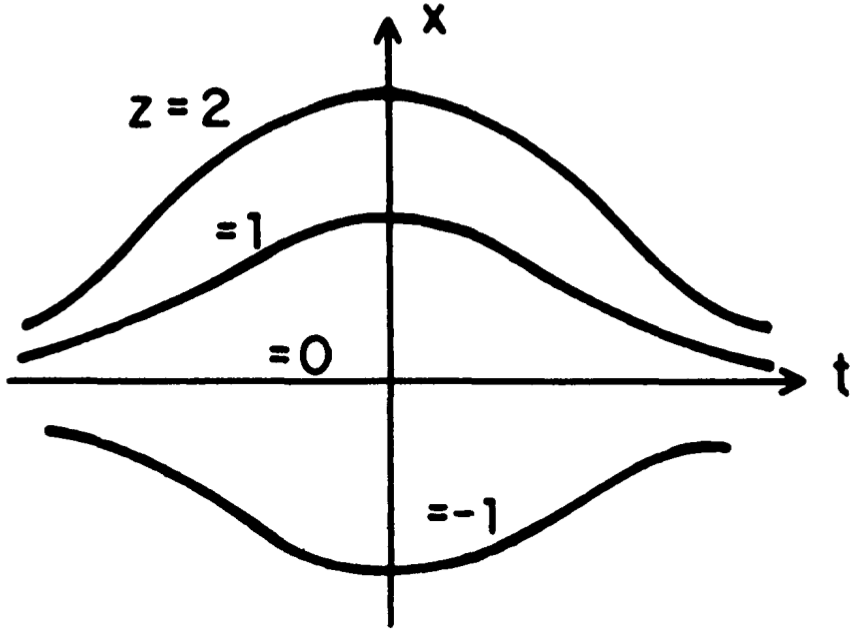
\includegraphics[width=0.5\textwidth]{instantonfig9.png}
    \caption{ \label{instantonfig9}}
  \end{figure}
\begin{tcolorbox}
    \begin{remark}
        这里稍微做一些解释. 我们把这个路径上的函数记为$x(z,t)$. 上面的条件相等于说$x(0,t)=0$以及$x(1,t)$是回弹解. 更进一步, 我们在$x(1,t)$附近展开作用量$S$:
        \[
        S(x(z,t))= S(x(1,t))+(x(z,t)-x(1,t))  \cdot \frac{\delta^{2}S}{\delta x^{2}}\biggr\vert_{x=x(1,t)}\cdot (x(z,t)-x(1,t))  
        \]
        这里的一阶导数由于经典运动方程为零, 而$(x(z,t)-x(1,t))=(z-1)\partial_{z}x(1,t)$, 我们把$\partial_{z}x(1,t)$展到$\delta^{2}S/\delta x^{2}$的本征函数, 这些本征函数只有$x_{0}$的本征值为负, 在这个方向上,
        \[
            S(x(z,t))=   S(x(1,t))-c_{0}\bigl((z-1)x_{0}\bigr)^{2}.
        \]
        因为$c_{0}$为正, 所以$S$迅速减小, 那么$\exp(-S/\hbar)$会指数增长, 因此称其为最危险的方向.
    \end{remark}    
\end{tcolorbox}
\noindent 随着$z$趋于无穷, 由于函数在转折点之后($V<0\,$)区域停留的时间越来越长, $S$趋于负无穷大; 这暗示了方程\eqref{instanton2.51}发散的很厉害.

\begin{figure}[h]
    \centering
    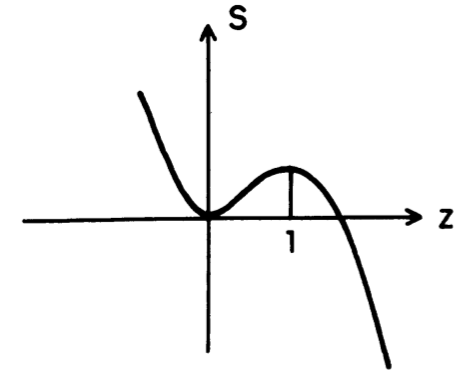
\includegraphics[width=0.5\textwidth]{instantonfig10.png}
    \caption{ \label{instantonfig10}}
  \end{figure}

如果$x=0$是$V$的绝对最小值, 这就是说, 如果$V$如图\ref{instantonfig11}(a)所示, 对于函数空间的同一路径, 情况将如图\ref{instantonfig11}(b)所示, 也就不会有方程\eqref{instanton2.48}中的发散. 现在我们解析地改变$V$使得我们从这个情况回到感兴趣的情况. 为了保持积分收敛, 我们必须把积分围道的右半端扭到复平面中. 如何改变积分围道依赖于如何将一个势变到另一个势的解析细节. 在图\ref{instantonfig12}中, 我们假定积分围道被扭到了上半平面. 使用最速下降法的标准处理, 将围道选取成: 沿着实轴从负无穷到鞍点$z=1$, 然后跑到复平面. 这个积分也就获得了虚部; 在最速下降的近似中
\begin{align}
    \operatorname{Im} J &= \operatorname{Im} \int_{1}^{1+\mi\infty} \dif z\: (2\pi\hbar)^{-1/2} \exp\Bigl(-S(1)/\hbar- \tfrac{1}{2}S''(1)(z-1)^{2}/\hbar\Bigr) \nonumber \\
    &=\tfrac{1}{2}\me^{-S(1)/\hbar} \bigl\lvert S''(1)\bigr\rvert^{-1/2} \:. \label{instanton2.52}
\end{align}
注意这个$\tfrac{1}{2}$因子; 它出现是因为积分围道只取了高斯峰的一半. (如果把积分围道扭到下半平面, 那么这个虚部就会有一个额外的符号).

\begin{figure}[h]
    \centering
    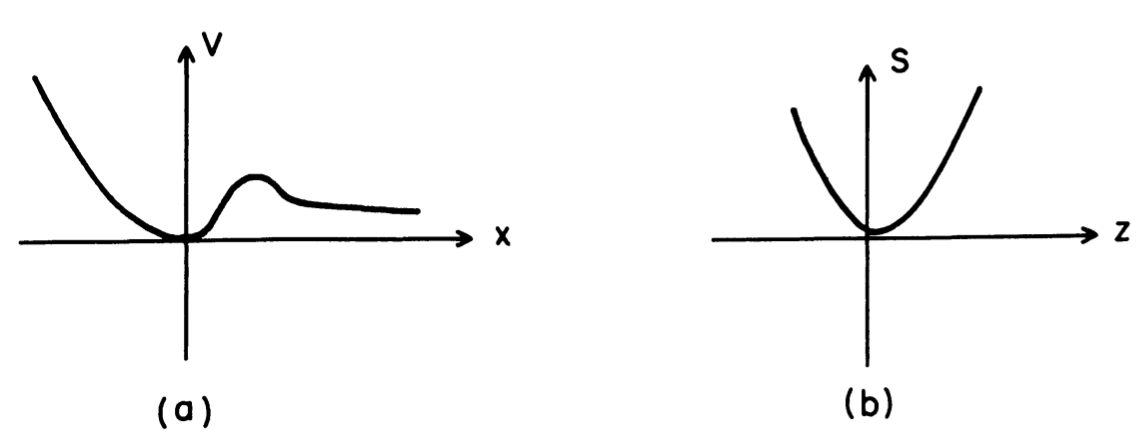
\includegraphics[width=0.9\textwidth]{instantonfig11.png}
    \caption{ \label{instantonfig11}}
  \end{figure}

  \begin{figure}[h]
    \centering
    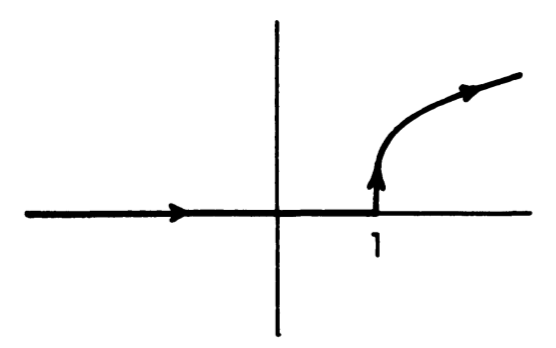
\includegraphics[width=0.5\textwidth]{instantonfig12.png}
    \caption{ \label{instantonfig12}}
  \end{figure}

我们到现在为止所研究的都是一维积分, 但由于与路径垂直的方向所联系的本征值都是非负的, 所以它们的泛函积分是平庸的. 以这种方式我们就获得了沙格列托的结果\eqref{instanton2.49}, 不同之处是对于负本征值有一个额外的$\tfrac{1}{2}$因子.


\section{规范场论中的真空结构}

\subsection{冷饭} \label{instanton:sec3.1}

这个小节主要回顾规范场论的一些基本知识, 并确定一些符号约定.

\paragraph*{李代数} 李代数的表示是$N$个反厄密矩阵$T^{a}$, $a=1,\ldots,N$, 的集合, 他们满足方程
\begin{equation}
    [T^{a},T^{b}]= c^{abc} T^{c} \:, \label{instanton3.1}
\end{equation}
其中$c$是某个紧李群$G$的结构常数. 总可以选择$T$使得$\operatorname{Tr}(T^{a}T^{b})$正比于$\delta^{ab}$, 而比例常数可能正比于表示. 嘉当内积定义成
\begin{equation}
    (T^{a},T^{b}) = \delta^{ab} \:. \label{instanton3.2}
\end{equation}
因此它正比于矩阵乘积的迹.

接下来来确定结构常数和$T$. 对于主要要处理的$SU(2)$, 选择$c^{abc}$为$\varepsilon^{abc}$. 因此, 对于同位旋表示,
\begin{equation}
    T^{a} = -\mi\sigma^{a}/2 \:, \label{instanton3.3}
\end{equation}
其中$\sigma$是泡利矩阵. 在这个情况下,
\begin{equation}
    (T^{a},T^{b})=-2\operatorname{Tr}(T^{a}T^{b}) \:. \label{instanton3.4}
\end{equation}

我们偶尔会讨论$SU(n)$, 特别是$SU(3)$. 对于它们, 结构常数和$T$的选择会使得它们对$SU(2)$子群与上面的选择相同. 因此, 对于$SU(3)$, $T^{a}$是$-\mi\lambda^{a}/2$, 其中$\lambda$是盖尔曼矩阵.

\paragraph*{规范场} 规范势是一组矢量场$A_{\mu}^{a}(x)$. 接下来定义矩阵值矢量场$A_{\mu}(x)$,
\begin{equation}
    A_{\mu}=gA_{\mu}^{a}T^{a} \:, \label{instanton3.5}
\end{equation}   
其中$g$是规范耦合常数. 场强张量$F_{\mu\nu}(x)$定义成
\begin{equation}
    F_{\mu\nu} = \partial_{\mu}A_{\nu}- \partial_{\nu}A_{\mu} + [A_{\mu},A_{\nu}] \:. \label{instanton3.6}
\end{equation}
纯规范场理论的欧几里得作用量是
\begin{equation}
    S= \frac{1}{4g^{2}} \int \dif^{4}x\: (F_{\mu\nu},F_{\mu\nu}) \:. \label{instanton3.7}
\end{equation}
有时简写成
\begin{equation}
    S=\frac{1}{4g^{2}} \int (F^{2}) \:. \label{instanton3.8}
\end{equation}

\paragraph*{规范变换} 规范变换是一个从欧几里得空间到规范群$G$的函数$g(x)$. 写成方程就是
\begin{equation}
    g(x) = \exp \bigl( \lambda^{a}(x)T^{a}\bigr) \:, \label{instanton3.9}
\end{equation}
其中$\lambda$是任意函数. (这里不要与耦合常数$g$相混淆.) 在这样一个变换下
\begin{equation}
    A_{\mu} \to g A_{\mu} g^{-1} +g \partial_{\mu} g^{-1} \:, \label{instanton3.10}
\end{equation}
以及
\begin{equation}
    F_{\mu\nu} \to g F_{\mu\nu} g^{-1} \:. \label{instanton3.11}
\end{equation}
因此$S$是规范不变的. 如果$F_{\mu\nu}$为零, 那么$A_{\mu}$是0的规范变换; 这就是说
\begin{equation}
    A_{\mu} = g\partial_{\mu}g^{-1} \:. \label{instanton3.12}
\end{equation}

\paragraph*{协变导数} 场强张量的协变导数定义成
\begin{equation}
    D_{\lambda}F_{\mu\nu} = \partial_{\lambda}F_{\mu\nu} + [A_{\lambda}, F_{\mu\nu}] \:. \label{instanton3.13}
\end{equation}
作用量\eqref{instanton3.7}给出运动方程
\begin{equation}
    D_{\mu} F_{\mu\nu} =0 \:. \label{instanton3.14}
\end{equation}
对于给定的场$\psi$, 假定它服从规范变换
\begin{equation}
    \psi \to g(x) \psi \:, \label{instanton3.15}
\end{equation}
那么$\psi$的协变导数
\begin{equation}
    D_{\mu}\psi = \partial_{\mu} \psi +A_{\mu} \psi
\end{equation}
以相同方式进行变换.

\subsection{缠绕数}

我们为什么研究作用量是有限值的规范场构型? 想当然的答案是, 作用量无限大的场构型有$\me^{-S/\hbar}=0$, 所以它们对泛函积分是不重要的. {\kaishu{这是错的}}. 实际上有限作用量的构型不重要; 更确切一些, 它们是函数空间的零测集. 我们对作用量有限的场构型感兴趣的唯一原因是我们想做半经典近似, 而如果我们把作用量无限大的场构型选做高斯积分的中心点, 那么它确实会给出零.
\begin{tcolorbox}
  \begin{remark}
    这里用有限维空间中的鞍点近似法来做一些解释说明:
    \begin{equation*}
        \int_{\mathbb{R}^{n}} g(x)\me^{\mi k f(x)} \dif x \simeq \sum_{x_{0}\in \Sigma} \me^{\mi k f(x_{0})}
        \bigl| \det (\operatorname{Hess}(f))\bigr|^{-1/2} \me^{\pi\mi \operatorname{sgn}(\operatorname{Hess}(f))/4}
        \biggl(\frac{2\pi}{k}\biggr)^{n/2}g(x_{0})
    \end{equation*}
这里的$\operatorname{Hess}(f)$是指$\partial^{2} f/\partial x_{i}\partial x_{j}$构成的海赛矩阵, 而$\operatorname{sgn}(\operatorname{Hess}(f))$是海赛矩阵的正本征值个数与负本征值个数之差, $\Sigma$则是临界点的个数.

上面所说的``有限作用量的构型是函数空间的零测集''就等同于这里的$\Sigma$是$\mathbb{R}_{n}$的零测集, 诚然在上式右边去掉这些临界点并不会对积分有影响, 但这里实际上关心的是积分关于临界点的展开, 而这样的展开仅在$k\to \infty$时才是有效的.
  \end{remark}  
\end{tcolorbox}

作用量积分的收敛性是由$A_{\mu}$在$r$很大时的行为决定的, 其中$r$是欧几里得空间中的径向变量. 为了使讨论尽可能简单, 假定$r$很大时, $A_{\mu}$可以展成$r$的负幂次的渐进级数. 因此为了使作用量有限, $F_{\mu\nu}$在$r$很大时必须比$1/r^{2}$衰减得要快; 这就是说, $F_{\mu\nu}$必须是$O(1/r^{3})$. 这暗示了$A_{\mu}$是$O(1/r^{2})$, 但这还不完全: $F_{\mu\nu}$为零只能给出$A_{\mu}$是零的规范变换. 因此$A_{\mu}$形如
\begin{equation}
    A_{\mu} = g \partial_{\mu} g^{-1} + O(1/r^{2}) \:, \label{instanton3.17}
\end{equation}
其中$g$是从4维空间到群$G$的$O(1)$函数, 这就是说, 它是角变量的函数.

\begin{remark}
这里的$g(x)$是紧群$G$上的元素, 所以它最多是$O(1)$的, 我们这里只关心$A_{\mu}$在$r\to\infty$时行为, 所以$g$只需要是角变量的函数.    
\end{remark}

因此, 每个作用量有限的场构型都会联系到角变量的一个群元值函数, 也就是说, 一个三维超球面$S^{3}$到规范群$G$的映射. 当然, 这个分配不是规范不变的. 在规范变换$h(x)$下,
\begin{equation}
    A_{\mu } \to h A_{\mu}h^{-1} + h \partial_{\mu}h^{-1} \:. \label{instanton3.18}
\end{equation}
因此,
\begin{equation}
    g\to hg + O(1/r^{2}) \:. \label{instanton3.19}
\end{equation}
\begin{tcolorbox}
    把方程\eqref{instanton3.17}代入\eqref{instanton3.18}右边, 得到
    \begin{align*}
        A_{\mu} &\to hg(\partial_{\mu}g^{-1})h^{-1} +h\partial_{\mu}h^{-1} \\
        &= hg \Bigl( (\partial_{\mu}g^{-1})h^{-1} +g^{-1}\partial_{\mu}h^{-1}\Bigr) =hg \partial_{\mu} (g^{-1}h^{-1}) \:. 
    \end{align*}
    即方程\eqref{instanton3.19}
\end{tcolorbox}

如果我们能选择$h$使得它在无穷远处等于$g^{-1}$, 我们可以把$g$变换到1然后从方程\eqref{instanton3.17}中消掉它. 然而, 这一般是不可能的. 
原因是$h$不仅要是无穷远处的超球面上的连续函数, 也得在整个四维空间连续, 也就是说, 沿着$r$把整个四维空间划成逐层嵌套的超球面, 在这些连续变换的超球面上, $h$是连续的. 特别地, $h$在原点必须是一个常数. 因此, 无穷远处的$h$不可能是$S^{3}$上的一般函数, 而是可以通过连续形变可以从常函数得到的连续函数. 由于任何常数规范变换都可以从恒等变换做连续形变得到(所有规范群都是连通的), 我们也可以说无穷远处的$h$可以通过对$h=1$做连续形变得到.

给定从一个拓扑空间到另一个拓扑空间的两个映射, 如果一个映射可以连续形变到另一个, 数学家称这两个函数是“同伦的”或者“处在同一个同伦类中”. 我们刚才证明了我们可以通过规范变换把$g(x)$变换到任何与$g(x)$同伦的映射, 但我们无法把它变换到另一个同伦类中的函数. 因此, 与有限作用量场构型相联系的不是$S^{3}$到$G$的映射, 而是这种映射的同伦类. 我们的任务是对物理上感兴趣的$G$找到这些同伦类.

我们先来做个热身练习, 考虑一个几何可视化的简化版. 我们将处理最简单的规范群, $U(1)$. 这样规范场论就是普通的电磁理论. (然而, 我们这里所采用的符号约定是\ref{instanton:sec3.1}节中确定的那些, 因此$A_{\mu}$将是纯虚的.) 另外, 我们将考虑二维空间而不是四维空间. 我们仍然要研究满足方程\eqref{instanton3.17}的场, 尽管这个条件不再是作用量有限的结果. 由于我们处理的是二维空间, 所以取代前面的超球面$S^{3}$, 我们这里面对的是一个圆$S^{1}$.

现在开始处理:
\begin{enumerate}
    \item $G$是复平面中的单位圆; 因此, 从拓扑上将, $G$也是$S^{1}$, 所以我们必须研究从$S^{1}$到$S^{1}$的映射的同伦类. 我们将按照传统方式用在$0$到$2\pi$之间取值的$\theta$来标记空间中的圆, 即映射的定义域.
    \item 定义一些从$S^{1}$到$S^{1}$的标准映射. 一个是平庸映射,
    \begin{subequations} \label{instanton3.20}
        \begin{gather}
            g^{(0)}(\theta)=1 \:. \label{instanton3.20a} \\
        \intertext{另一个是单位映射,}
            g^{(1)}(\theta) = \me^{\mi\theta} \:. \label{instanton3.20b}\\
        \intertext{它们都是如下映射族}
            g^{(\nu)}(\theta) = [g^{(1)}(\theta)]^{\nu} = \me^{\mi\nu\theta}  \tag{3.20c} \label{instanton3.20c} 
        \end{gather}  
    \end{subequations}
    的成员, 其中$\nu$是整数. $\nu$被称为``缠绕数''.
    \item 每个从$S^{1}$到$S^{1}$的映射同伦于映射\eqref{instanton3.20c}中的一个. 这是著名的事实$\pi_{1}(S^{1})=\mathbb{Z}$. 即圆的第一同伦群是整数加法群.
    \item 上述缠绕数可以有如下积分公式给出:
    \begin{equation}
        \nu = \frac{\mi}{2\pi} \int_{0}^{2\pi} \dif\theta\: g\frac{\dif }{\dif\theta} g^{-1}\:. \label{instanton3.21}
    \end{equation}
    对于标准映射\eqref{instanton3.20c}, 这显然是成立的. 这个量在连续变换下也是不变的. 这点可以通过考虑无限小形变来证明. 一个无限小的形变可以写成
    \begin{equation}
        \delta g =\mi (\delta\lambda) g\:, \label{instanton3.22}
    \end{equation}
    其中$\delta\lambda$是圆上的无限小实函数. 因此
    \begin{align}
        \delta\biggl(g\frac{\dif}{\dif\theta} g^{-1}\biggr) &= (\delta g)\frac{\dif}{\dif\theta} g^{-1}+
        g\frac{\dif}{\dif\theta} (\delta g^{-1})=\mi\delta \lambda \,g \frac{\dif}{\dif\theta} g^{-1} 
        -\mi g \frac{\dif}{\dif\theta} (\delta\lambda\,g^{-1}) \nonumber \\
        &=-\mi \frac{\dif}{\dif\theta} \delta\lambda \label{instanton3.23}
    \end{align}
    这里使用了$\delta g^{-1}= -g^{-1}(\delta g) g^{-1}$, 由此看出这不会对$\nu$产生影响.
    \item 如果
    \begin{subequations}
        \begin{gather}
        g(\theta) = g_{1}(\theta)g_{2}(\theta) \:, \tag{3.24a} \label{instanton3.24a} \\
    \intertext{那么}
        \nu= \nu_{1}+\nu_{2} \:. \tag{3.24b} \label{instanton3.24b}
        \end{gather}
    \end{subequations}
    证明是简单的: 对$g_{1}$做形变使得它在上半圆为1, 对$g_{2}$做形变使得它在下半圆为1.
    \item 我们定义
    \begin{equation}
        G_{\mu} =\frac{\mi}{2\pi} \varepsilon_{\mu\nu} A_{\nu} \:. \label{instanton3.25}
    \end{equation}
    通过方程\eqref{instanton3.17}和\eqref{instanton3.21},
    \begin{equation}
        \nu = \lim_{r\to\infty} \int_{0}^{2\pi} r \dif \theta\: \hat{r}_{\mu}G_{\mu} \:, \label{instanton3.26}
    \end{equation}
    其中$\hat{r}_{\mu}$是径向单位矢量. 因此通过高斯定理,
    \begin{equation}
        \nu = \int\dif^{2}x\: \partial_{\mu}G_{\mu} \:. \label{instanton3.27}
    \end{equation}
    这样,
    \begin{equation}
        \nu = \frac{\mi}{4\pi}\int\dif^{2}x\: \varepsilon_{\mu\nu}F_{\mu\nu} \:. \label{instanton3.27}
    \end{equation}
    \begin{remark}
        这里使用了$\hat{r}_{\mu}\varepsilon_{\mu\nu}A_{\nu}=\cos\theta A_{y}-\sin\theta A_{x}= r^{-1} g\partial_{\theta} g^{-1}$
    \end{remark}
\end{enumerate}

\subsection{多个真空}

\subsection{瞬子: 一般情形}

\subsection{瞬子: 特殊情形}

\section{$1+1$维中的阿贝尔Higgs模型}



\section{$U(1)$问题的't Hooft解决方案}

\subsection{介子失踪之谜}

\subsection{准备工作: 欧几里得费米场}

\subsection{准备工作: 手征沃德恒等式}

\subsection{QCD(幼儿版)}


\subsection{QCD(真实版)}

\subsection{杂录}


\section{假时空的命运}

\subsection{不稳定真空}

\subsection{回弹}

\subsection{薄壁近似}

\subsection{假真空的命运}

\subsection{行列式与重整化}

\subsection{待解答的问题} %% Notes on Coleman "The uses of Instanton" 

\setcounter{chapter}{14}
\counterwithin*{footnote}{section}
%\renewcommand*\thesection{\arabic{section}}
\setcounter{section}{0}%更改chapter的计数器值
%\numberwithin{equation}{chapter}%公式计数器从属于节计数器
\numberwithin{equation}{section}%公式计数器从属于节计数器
\numberwithin{figure}{chapter}%图计数器从属于节计数器
%\renewcommand*\thefigure{\arabic{section}}

\chapter{非阿贝尔规范场论} \label{cha:15}
% \thispagestyle{empty}
% \marginpar[\flushright
% {\raisebox{17ex}[0pt]{{\small[1]\hspace*{5mm}}}}]{{\raisebox{17ex}[0pt]{\small\hspace*{5mm}[1]}}}
% \setcounter{page}{1}
% \pagenumbering{arabic}
%  \markboth{第15章\quad 非阿贝尔规范场论}{第15章\quad 非阿贝尔规范场论}


被证实了的成功描述真实世界的量子场论都是非阿贝尔规范理论, 这些理论所基于的规范不变性原理要比量子电动力学的$U(1)$规范不变性更加普遍. 
对电动力学, 我们在8.1节的末尾概述了如何从定域变换下的不变性原理出发得到规范场的存在性以及它的一些性质, 
而非阿贝尔规范理论同样具有这一迷人的特征. 
在电动力学中, 电荷为$e_{n}$的场$\psi _{n}(x)$进行了$\Lambda(x)$为任意函数的规范变换
$\psi _{n}(x)\to \exp(\mi e_{n}\Lambda (x))\psi _{n}(x)$. 
由于$\partial _{\mu }\psi _{n}(x)$并不像$\psi_{n}(x)$那样变换, 
我们必须要引入具有规范变换性质$A_{\mu }(x)\to A_{\mu}(x)+\partial_{\mu}\Lambda(x)$的场$A_{\mu}(x)$, 
用它来构建规范协变导数$\partial_{\mu}\psi_{n}(x)-\mi e_{n}A_{\mu}(x)\psi_{n}(x)$, 
这一协变导数像$\psi _{n}(x)$那样变换, 因而可以用它和$\psi_{n}(x)$构造规范不变的拉格朗日量. 
用类似的方法, 从广义坐标变换下的对称性原理可以得到广义相对论中的引力场$g_{\mu \nu }(x)$的存在性以及一些性质.\footnote{当然, 
定域规范不变性与广义协变性都可以以一种平庸的方式实现, 即把$A_{\mu }(x)$
和$g_{\mu \nu }(x)$分别取作用以确定相位和坐标系选取的非动力学c-数函数. 
当我们将$A_{\mu }(x)$和$g_{\mu \nu }(x)$处理成在计算$S$-矩阵元时要对其积分的动力学场时, 
这些对称性在物理上就变得重要了.} 有了这些著名的先例后, 将定域规范不变性推广到定域非阿贝尔规范变换下的不变性就很自然了.


在杨振宁和Mills 1954年的原始工作中,\cite{1} 非阿贝尔规范群被取成了同位旋转动的$SU(2)$群, 
而类似于光子场的矢量场则解释成强相互作用的单位同位旋矢量介子场. 这一设想立刻就遇到了障碍: 
就像光子那样, 这些矢量玻色子的质量必须为零, 而任何这样的粒子如果存在, 那它们似乎早就该被探测到了. 
另一问题是, 像当时所有的强相互作用理论一样, 没有什么方法可以处理它; 
理论中的大耦合常数似乎妨碍了任何微扰论的应用.

规范理论不久就被推广至任意的非阿贝尔规范群,\cite{2} 并且继续在数学上研究它们的量子化, 
尤其是Feynman,\cite{3} Faddeev和Popov,\cite{4} 以及De Wittt,\cite{5} 部分的出发点是作为更困难的广义相对论量子化问题的热身. 
他们证明了那些通过简单观察拉格朗日量得到的朴素的Feynman规则需要补上额外的``鬼''圈. 
然而, 直到20世纪60年代后期, 这些理论在物理上的联系才开始被理解. 
最后发现, {\kai{所有}}观测到的基本粒子间的相互作用都是由伴随定域规范对称性的矢量粒子生成的; 
相应的自旋1粒子要么非常重, 这是规范对称性自发破缺的结果, 要么被``禁闭''了, 这是耦合常数在远距离处变大的结果. 
这些内容将分别是第21章和第18章的课题. 在本章, 我们将探讨非阿贝尔规范理论的表述, 以及如何推导它们的Feynman规则.

\section{规范不变性}

\setcounter{footnote}{1}

我们假定理论的拉格朗日量在物质场$\psi _{\ell }(x)$的一组无限小变换
\begin{equation}
\deltaup \psi _{\ell }(x)=\mi\,\epsilon ^{\alpha }(x)(t_{\alpha })_{\ell }{}^{m}\psi _{m}(x)  \label{15.1.1}
\end{equation}%
下不变, 其中$t_{\alpha }$为某组独立的常数矩阵\footnote{%
在本书中, 我们一般将用字母$\alpha ,\beta $等来标记对称性的生成元, 这些字母取自希腊字母表的开头, 
以区别于取自希腊字母表中间的用来标记时空坐标的$\mu ,\nu $等字母. 在后面处理破缺对称性时, 
我们通常用取自拉丁字母表开头的字母$a,b$等来标记自发破缺对称性的生成元, 而用取自拉丁字母表中%
间的字母$i,j$等来标记未破缺的对称性的生成元.}, 
$\epsilon ^{\alpha}(x)$是实无限小参量, 该参量(像电动力学中的规范变换那样)可以依赖时空中的位置. 
我们假定这些对称变换是某个Lie群的无限小部分; 正如2.2节中所证明的, 这要求$t_{\alpha}$服从对易关系
\begin{equation}
[ t_{\alpha },t_{\beta }]=\mi\, C^{\gamma}{}_{\alpha \beta }t_{\gamma}\:,  \label{15.1.2}
\end{equation}%
其中$C_{\phantom{\gamma}\alpha \beta }^{\gamma }$是一组实常数, 称为群的结构常数. 
由对易子的反对称性立刻就可以知道, 结构常数同样是反对称的:%
\begin{equation}
C^{\gamma}{}_{\alpha\beta}=-C^{\gamma}{}_{\beta\alpha} \:. \label{15.1.3}
\end{equation}%
另外, 由Jacobi恒等式
\begin{equation}
0=\Bigl[ [t_{\alpha},t_{\beta}],t_{\gamma}\Bigr] + \Bigl[ [t_{\beta},t_{\gamma }],t_{\alpha }\Bigr] 
+\Bigl[ [t_{\gamma },t_{\alpha }],t_{\beta}\Bigr]  \label{15.1.4}
\end{equation}%
我们看到这些$C$满足进一步的约束
\begin{equation}
0=C^{\delta }{}_{\alpha \beta }C^{\epsilon}{}_{\delta\gamma}
+C^{\delta}{}_{\gamma \alpha}C^{\epsilon}{}_{\delta \beta }
+C^{\delta }{}_{\beta \gamma}C^{\epsilon }{}_{\delta \alpha}  \:. \label{15.1.5}
\end{equation}%
任何一组满足方程(\ref{15.1.3})和(\ref{15.1.5})的常数${C^{\gamma}}_{\alpha\beta}$定义了至少一组矩阵${t^{\text{A}}}_{\alpha}$:%
\begin{equation}
{({t^{\text{A}}}_{\alpha})^{\beta}}_{\gamma }\equiv -\mi\,{C^{\beta }}_{\gamma \alpha } \:,
\label{15.1.6}
\end{equation}%
它们满足含有结构常数$C_{\phantom{\gamma}\alpha \beta }^{\gamma }$的对易关系(\ref{15.1.2}):%
\begin{equation}
[ {t^{\text{A}}}_{\alpha},{t^{\text{A}}}_{\beta}]=\mi\,C^{\gamma}{}_{\alpha \beta }{t^{\text{A}}}_{\gamma}\:.   \label{15.1.7}
\end{equation}%
这被称作结构常数为$C^{\alpha}{}_{ \beta\gamma }$的Lie群的 ``伴随'' (或 ``正则'' )表示.

例如, 在原始的Yang-Mills理论中, 物质场是由质子场$\psi_{p}$和中子场$\psi_{n}$组成的双重态
\[
\psi =
\begin{pmatrix}
\psi _{p} \\
\psi _{n}%
\end{pmatrix}%
\]
而$t_{\alpha }$, 其中$\alpha =1,2,3$, 是同位旋矩阵
\[
t_{1}=\frac{1}{2}\begin{pmatrix}
    0 & 1 \\
    1 & 0%   
\end{pmatrix} \:, \qquad 
t_{2}=\frac{1}{2}\begin{pmatrix}
    0 & -\mi \\
\mi & 0%
\end{pmatrix} \:,\qquad 
t_{3}=\frac{1}{2}\begin{pmatrix}
    1 & 0 \\
    0 & -1%  
\end{pmatrix} \:.
\]%
它们所满足的对易关系(\ref{15.1.2})有
\[
C^{\gamma}{}_{\alpha \beta}=\epsilon _{\gamma \alpha \beta } \:,
\]%
其中, 像通常那样, 当$\gamma ,\alpha ,\beta $是1,2,3的偶置换或奇置换时,
$\epsilon _{\gamma \alpha \beta }$分别是$+1$或$-1$, 其它情况下, $\epsilon _{\gamma \alpha \beta }$为零. 
我们发现这与3维旋转群的Lie代数(2.4.18)相同; 这里的矩阵构成了我们所说的该Lie代数的自旋1/2表示. 
伴随表示的矩阵(\ref{15.1.6})在这里是(在行和列标记为1,2,3的基下):%
\[
t_{1}^{\text{A}}=\begin{bmatrix}
0 & 0 & 0 \\
0 & 0 & -\mi \\
0 & \mi & 0%
\end{bmatrix}  \: ,\qquad 
t_{2}^{\text{A}}=\begin{bmatrix}
    0 & 0 & \mi \\
    0 & 0 & 0 \\
    -\mi & 0 & 0% 
\end{bmatrix} \:, \qquad 
t_{3}^{\text{A}}=
\begin{bmatrix}
    0 & -\mi & 0 \\
\mi & 0 & 0 \\
0 & 0 & 0%
\end{bmatrix} \:.
\]%
这是旋转群Lie代数的自旋1表示.

我们现在考虑构造一个在变换(\ref{15.1.1})下不变的拉格朗日量需要什么. 如果没有场的导数项, 
这个任务是很简单的——物质场的任何函数, 只要它在$\epsilon ^{\alpha }$为常数的变换(\ref{15.1.1})下不变, 
那么在$\epsilon ^{\alpha }$为时空坐标的任意实函数时, 它在变换(\ref{15.1.1})下也将是不变的. 
如果拉格朗日量包含场的导数项(正如它所必须的)就不会是这种情况, 这是因为有了依赖位置的函数$\epsilon ^{\alpha }(x)$,
物质场的导数就不会像场本身那样变换. 对方程(\ref{15.1.1})两边做微分给出
\begin{equation}
\deltaup \Big( \partial _{\mu }\psi _{\ell }(x)\Big) =\mi\,\epsilon ^{\alpha
}(x)(t_{\alpha })_{\ell }{}^{m}\Big( \partial _{\mu }\psi
_{m}(x)\Big) +\mi\Big( \partial _{\mu }\epsilon ^{\alpha }(x)\Big)
(t_{\alpha })_{\ell}{}^{m}\psi _{m}(x)\:.  \label{15.1.8}
\end{equation}%
为了使拉格朗日量不变, 我们需要一个场$A^{\alpha }{}_{\mu }$, 它的变换规则中包含一项$\partial _{\mu }\epsilon
^{\alpha }$, 这一项可以用来抵消方程(\ref{15.1.8})中的第二项. 既然这个场携带了一个$\alpha $指标, 我们希望它%
也经历一个类似方程(\ref{15.1.1})的矩阵变换, 所不同的只是把$t_{\alpha }$替换成伴随矩阵表示(\ref{15.1.6}). 因此, 
我们先尝试着取新``规范'' 场的变换关系为
\[
\deltaup A^{\beta}{}_{\mu }=\partial _{\mu }\epsilon ^{\beta}+
\mi\,\epsilon ^{\alpha }({t^{\text{A}}}_{\alpha })^{\beta}{}_{\gamma}A^{\gamma}{}_{\mu }
\]%
或, 利用方程(\ref{15.1.6}),%
\begin{equation}
\deltaup A^{\beta }{}_{\mu }=\partial _{\mu }\epsilon ^{\beta
}+C^{\beta}{}_{\gamma \alpha }\epsilon ^{\alpha }A^{\gamma}{}_{\mu }\:. \label{15.1.9}
\end{equation}%
这使我们可以构造出 ``协变导数'' :%
\footnote{正如将要在下一节讨论的, 写下方程(\ref{15.1.10})的同时, 我们默认假定任何像电荷这样的耦合常数因子都被吸收进$t_{\beta }$中,
从而也被吸收进结构常数中.}%
\begin{equation}
\big(D_{\mu }\psi (x)\big)_{\ell }=\partial _{\mu }\psi _{\ell }(x)
-\mi\,A^{\beta}{}_{\mu }(x)(t_{\beta })_{\ell}{}^{m}\psi_{m}(x) \:.  \label{15.1.10}
\end{equation}%
和预想的一样, 方程(\ref{15.1.10})第二项中${A^{\beta }}_{\mu }$变换中的$\partial _{\mu }\epsilon ^{\beta }$项%
抵消了第一项变换中正比于$\partial _{\mu }\epsilon ^{\beta }$的那项, 给我们留下\begin{align*}
\deltaup (D_{\mu }\psi )_{\ell } &=\mi\,\epsilon ^{\alpha }\,(t_{\alpha })_{\ell }^{%
\phantom{\ell}m}\,\partial _{\mu }\psi _{m}-\mi\,{C^{\beta }}_{\gamma \alpha
}\,\epsilon ^{\alpha }\,{A^{\gamma }}_{\mu }\,(t_{\beta
})_{\ell }^{\phantom{\ell}m}\,\psi _{m} \\
&\quad+{A^{\gamma }}_{\mu }\,(t_{\gamma })_{\ell }^{\phantom{\ell}%
m}\,(t_{\alpha })_{m}^{\phantom{m}n}\,\psi _{n}\, \epsilon^{\alpha}
\end{align*}%
或利用方程(\ref{15.1.2}),%
\begin{equation}
\deltaup (D_{\mu }\psi )_{\ell }=\mi\,\epsilon ^{\alpha }\,(t_{\alpha })_{\ell }^{%
\phantom{\ell}m}\,(D_{\mu }\psi )_{m}\:,  \label{15.1.11}
\end{equation}%
使得$D_{\mu }\psi $像$\psi $本身那样变换.

我们还需要关注一下规范场的导数. 为了消除$\partial _{\nu }{A^{\beta }}_{\mu }$变换中的
$\partial_{\nu}\partial _{\mu }\epsilon ^{\beta }$项, 像在电动力学中那样, 
我们对$\mu $和$\nu$做反对称化. 然而, 在$\partial _{\nu }{A^{\beta }}_{\mu }-\partial _{\mu }{A^{\beta }}_{\nu }$的变换中, 
仍有一些项正比于$\epsilon (x)$的一阶导数, 这些项来自方程(\ref{15.1.9})中的第二项. 在一个``协变旋度'' ${F^{\gamma }}_{\nu\mu}$的变换规则中, 所有这种$\epsilon (x)$的导数项都应该相互抵消, 而构造它最简单的方法就是考虑作用在物质场$\psi $上的两个协变导数的对易子:%
\begin{equation}
\Big( [ D_{\nu },D_{\mu }]\psi \Big) _{\ell }=-\mi\,(t_{\gamma })_{\ell
}^{\phantom{\ell}m}{F^{\gamma }}_{\nu\mu}\psi _{m}\:, 
\label{15.1.12}
\end{equation}%
其中\begin{equation}
{F^{\gamma }}_{\nu\mu}\equiv \partial _{\nu }{A^{\gamma }}_{\mu }-\partial _{\mu }{A^{\gamma }}_{\nu }+{C^{\gamma }}_{\alpha \beta }{A^{\alpha}}_{\nu }{A^{\beta }}_{\mu }\:.   \label{15.1.13}
\end{equation}%
从方程(\ref{15.1.12})中显而易见的是${F^{\gamma }}_{\nu \mu}$必须像伴随表示下的物质场那样进行变换:%
\begin{equation}
\deltaup\, {F^{\beta }}_{\nu \mu }\equiv \mi\,\epsilon ^{\alpha }({t^{\text{A}}}_{%
\alpha })^{\beta }{}_{\gamma }F^{\gamma}{}_{\nu \mu }
=\epsilon ^{\alpha }{C^{\beta }}_{\gamma \alpha }{F^{\gamma }}_{\nu \mu }\:.
\label{15.1.14}
\end{equation}%
读者可以通过直接计算(利用关系(\ref{15.1.5}))验证(\ref{15.1.13})中所定义的量${F^{\alpha }}_{\nu \mu }$确实具有简单的变换规则(\ref{15.1.14}).

由于某些原因, 知道这些无限小规范变换可以被升级为有限大变换是有用的. 群元可以被一组实函数$\Lambda ^{\alpha }(x)$%
参数化, 从而使它通过如下的矩阵变换作用在一个一般的物质场上\begin{equation}
\psi _{\ell }(x)\rightarrow \psi _{\ell \Lambda }(x)=\Big[ \exp \Big(
\mi\,t_{\alpha }\Lambda ^{\alpha }(x)\Big) \Big] _{\ell }^{\phantom{\ell}%
m}\psi _{m}(x)\:. \label{15.1.15}
\end{equation}%
我们希望协变导数以相同的方式进行变换:%
\begin{equation}
(\partial _{\mu }-\mi\,t_{\alpha }{A^{\alpha}}_{\mu \Lambda})\psi _{\Lambda
}=\exp (\mi t_{\alpha }\Lambda ^{\alpha })(\partial _{\mu }-\mi t_{\alpha }%
{A^{\alpha}}_{\mu })\psi \:,   \label{15.1.16}
\end{equation}%
所以我们必须在${A^{\alpha}}_{\mu}$上强加一个变换规则${A^{\alpha}}_{\mu }%
\rightarrow {A^{\alpha}}_{\mu \Lambda}$, 使得\[
\partial _{\mu }\exp (\mi t_{\beta }\Lambda ^{\beta })-\mi\,t_{\beta }\,\exp
(\mi t_{\alpha }\Lambda ^{\alpha }){A^{\beta}}_{\mu \Lambda}=-\mi\,\exp (\mi t_{\alpha
}\Lambda ^{\alpha })t_{\beta }{A^{\beta}}_{\mu}
\]%
或者, 换一种形式\begin{equation}
t_{\alpha }{A^{\alpha}}_{\mu \Lambda}=\exp (\mi t_{\beta }\Lambda ^{\beta
})t_{\alpha }{A^{\alpha}}_{\mu }\exp (-\mi t_{\beta }\Lambda ^{\beta })-\mi\Big[
\partial _{\mu }\exp (\mi t_{\beta }\Lambda ^{\beta })\Big] \exp (-\mi t_{\beta
}\Lambda ^{\beta })\:.   \label{15.1.17}
\end{equation}%
在$\Lambda ^{\alpha }(x)$是一个无限小$\epsilon ^{\alpha }(x)$的极限下, 方程(\ref{15.1.15})和(\ref{15.1.17})退化成前面的变换规则(\ref{15.1.1})和(\ref{15.1.9}).

我们从方程(\ref{15.1.17})中可以看到, 通过合适地选择$\Lambda ^{\beta }(x)$, 总可以使$%
{A^{\alpha}}_{\mu \Lambda}(x)$在任何{\kai{一个}}点处为零, 记该点$x=z$. (简单地令$\Lambda ^{\alpha }(z)$为零, 并在$x=z$处令$\partial \Lambda ^{\alpha }(x)/\partial x^{\mu}=-{A^{\alpha}}_{\mu }(x)$.) 另外, 总可以对$\Lambda ^{\beta }(x)$进行选择, 
使${A^{\alpha}}_{\mu \Lambda}(x)$的任意{\kai{一个}}时空分量对所有的$\alpha $至少在任意一个给定点邻近的有限区域内处处为零. 例如, 
为了使${A^{\alpha}}_{3 \Lambda}(x)$为零, 我们必须要解参量$\Lambda^{\beta }(x)$的如下一阶{\kai{常}}微分方程组:%
\begin{equation}
\partial _{3}\exp (\mi t_{\beta }\Lambda ^{\beta })=-\mi\exp (\mi t_{\beta }\Lambda
^{\beta })t_{\alpha }{A^{\alpha}}_{3 }\:,   \label{15.1.18}
\end{equation}%
该方程组至少在任意一个给定点邻近的有限区域内有一个解.

然而, 一般而言, 不可能通过选择$\Lambda ^{\alpha }(x)$使${A^{\alpha }}_{\mu \Lambda }(x)$的4个分量在一个有限区域内都为零. 为了这个目的, 我们将不得不去解{\kai{偏}}微分方程组\begin{equation}
\partial _{\mu }\exp (\mi t_{\beta }\Lambda ^{\beta })=-\mi\,\exp (\mi t_{\beta
}\Lambda ^{\beta })t_{\alpha }{A^{\alpha }}_{\mu }\:,   \label{15.1.19}
\end{equation}%
除非满足一定的可积性条件, 否则这个方程组是解不出来的. 特别地, 如果${A^{\alpha }}_{\mu \Lambda }$处处为零, 那么${F^{\alpha }}_{\mu \nu \Lambda }$也处处为零, 但是, 由于场强的变换是齐次的, 仅当${F^{\alpha }}_{\mu \nu }$为零时, ${F^{\alpha }}%
_{\mu \nu \Lambda }$才能等于零. 如果存在一个规范变换使得${A^{\alpha }}_{\mu }$处处为零,
则称该规范场为 ``纯规范'' 场. 不难证明, ${A^{\alpha }}_{\mu }(x)$在任意单连通区域可表示为纯规范场的充分必要条件正是${F^{\alpha }}_{\mu \nu }$处处为零.\cite{6}

\subsection*{* * *}

这里构造的在规范变换下进行简单变换的对象, 与在广义相对论中构造的在广义坐标变换下协变的对象之间存在着深刻的类比. 
正如我们用规范场构造规范变换性质与物质场相同的物质场协变导数$D_{\mu }\psi _{\ell }$, 
我们用仿射联络${\Gamma }{^{\mu }}_{\nu \lambda }(x)$来构造张量${T^{\rho \sigma \cdots }}_{\kappa
\lambda \cdots }$的协变导数:%
\begin{equation*}
T^{\rho \cdots}{}_{\kappa\cdots;\nu}\equiv \partial_{\nu}T^{\rho \cdots}{}_{\kappa\cdots}+\Gamma^{\rho}{}_{\nu\lambda}
T^{\lambda\cdots}{}_{\kappa\cdots}+\cdots-\Gamma^{\mu}{}_{\nu\kappa}T^{\rho\cdots}{}_{\mu\cdots}-\cdots \:, 
\end{equation*}
它们本身也是张量. 另外, 由规范场的导数, 我们构造出场强${F^{\alpha }}_{\mu
\nu }$, 它的规范变换性质与属于规范群伴随表示的物质场相同; 相应地, 仿射联络的导数可以构造一个量:%
\[
R{^{\lambda }}_{\mu \nu \kappa }=\frac{\partial {\Gamma }{^{\lambda }}_{\mu
\nu }}{\partial x^{\kappa }}-\frac{\partial {\Gamma }{^{\lambda }}_{\mu
\kappa }}{\partial x^{\nu }}+{\Gamma }{^{\eta }}_{\mu \nu }{\Gamma }{%
^{\lambda }}_{\kappa \eta }-{\Gamma }{^{\eta }}_{\mu \kappa }{\Gamma }{%
^{\lambda }}_{\nu \eta }\:, 
\]%
这个量按照一个张量变换, 即Riemann-Christoffel曲率张量. 两个规范协变导数$D_{\mu }$%
和$D_{\nu }$的对易子可以用场强张量${F^{\alpha }}_{\mu \nu }$表示; 类似地, 对$x^{\nu }$和$x^{\kappa }$的两个协变导数的对易子也可以用曲率
张量表示:%
\[
{T^{\lambda \cdots }}_{\mu \cdots ;\nu ;\kappa }-{T^{\lambda \cdots }}_{\mu
\cdots ;\kappa ;\nu }=R{^{\lambda }}_{\sigma \nu \kappa }{T^{\sigma \cdots }}%
_{\mu \cdots }+\cdots -R{^{\sigma }}_{\mu \nu \kappa }{T^{\lambda \cdots }}%
_{\sigma \cdots }-\cdots \:. 
\]%
存在一个规范, 使该规范下的规范场在一个有限单连通区域内为零的充要条件是场强张量为零, 而存在一个坐标系, 使仿射联络在一个%
有限单连通区域内为零的充要条件是Riemann-Christoffel曲率张量为零. 这个类比在一个重要方面上失效了: 
在广义相对论中, 仿射联络本身是由度规张量的一阶导数构造的, 而在规范理论中, 规范场无法用更基本的场表示.


\section{规范理论拉格朗日量与单Lie群}

规范场张量$F^{\alpha }{}_{\mu \nu }$, 物质场$\psi $以及它们的规范协变导数的变换规则不包含变换参%
量$\epsilon ^{\alpha }(x)$的导数, 所以如果只用这些元素构造拉格朗日量, 并且如果构造出的拉格朗日量在$\epsilon ^{\alpha }$为常数的%
整体变换下不变, 那么它在$\epsilon ^{\alpha }(x)$是位置的一般函数的规范变换下就是不变的. 因此,
我们假定拉格朗日量满足这些条件: 即,%
\begin{equation}
\mathscr{L}=\mathscr{L}(\psi ,D_{\mu }\psi ,D_{\nu }D_{\mu }\psi ,\cdots
,F^{\alpha }{}_{\mu \nu },D_{\rho }F^{\alpha }{}_{\mu \nu },、\cdots)  \label{15.2.1}
\end{equation}%
以及不变性条件:\begin{align}
&\frac{\partial \mathscr{L}}{\partial \psi _{\ell }}\,\mi(t_{\alpha })_{\ell }^{%
\phantom{\ell}m}\psi _{m}+\frac{\partial \mathscr{L}}{\partial (D_{\mu }\psi
_{\ell })}\,\mi(t_{\alpha })_{\ell }^{\phantom{\ell}m}(D_{\mu }\psi )_{m}
\nonumber \\
&+\frac{\partial \mathscr{L}}{\partial (D_{\nu }D_{\mu }\psi )_{\ell }}%
\,\mi(t_{\alpha })_{\ell }^{\phantom{\ell}m}(D_{\nu }D_{\mu }\psi )_{m}+\cdots +%
\frac{\partial \mathscr{L}}{\partial F^{\beta }{}_{\mu \nu }}C^{\beta}{}_{\gamma%
\alpha}F^{\gamma }{}_{\mu \nu }  \nonumber \\
&+\frac{\partial \mathscr{L}}{\partial D_{\rho }F^{\beta }{}_{\mu \nu }}%
C^{\beta}{}_{\gamma\alpha}D_{\rho }F^{\gamma }{}_{\mu \nu }+\cdots  =0%
\:.   \label{15.2.2}
\end{align}%
另一方面, 除了出现在$%
F^{\alpha }{}_{\mu \nu }$以及规范协变导数$D_{\mu }$中的规范场外, 拉格朗日量可以不依赖规范场本身. 特别地,
质量项$-\frac{1}{2}m^{2}{}_{\alpha\beta}A_{\alpha \mu}A_{\beta }{}^{\mu}$被排除了.

我们现在将要集中考察拉格朗日量中只依赖$F^{\alpha }{}_{\mu \nu }$的项. 如同在电动力学中一样, 对于任何自旋为一的无质量粒子, 
拉格朗日量必须包含一个自由粒子项, 这一项是$\partial _{\mu }A^{\alpha}{}_{\nu }-\partial _{\nu }A^{\alpha }{}_{\mu }$的二次项, 
而规范不变性则表明这一自由粒子项应该作为场强张量$F^{\alpha }{}_{\mu\nu}$的二次项的一部分出现. Lorentz不变性与宇称守恒表明它的形式为
\begin{equation}
\mathscr{L}_{A} = -\tfrac{1}{4}\, g_{\alpha\beta} F^{\alpha}{}_{\mu\nu} F^{\beta\mu\nu} \label{15.2.3}
\end{equation}
其中$g_{\alpha \beta }$是常数矩阵.
如果我们不假定宇称(%
或者$\mathsf{CP}$或\textsf{T})守恒, 那么拉格朗日量也可以包含如下的项%
\[
\mathscr{L}^{\prime}_{A} = -\tfrac{1}{2}\, \theta_{\alpha\beta} \,\epsilon^{\mu\nu\rho\sigma} F^{\alpha}{}_{\mu\nu} F^{\beta}{}_{\rho\sigma}
\]%
其中$\theta ^{\alpha \beta }$是另一个常数矩阵. 这一项实际上是全导数项, 因而并不影响场方程或Feynman规则. 然而, 这样的项会有%
非微扰的量子力学效应, 我们会在23.6节讨论它.

在继续考察矩阵$g_{\alpha \beta }$的性质之前, 注意到如下的事实是有价值的, 不引入相互作用, 就不可能引入规范场$A^{\alpha }{}_{\mu }
$的动能项, 方程(\ref{15.1.13})所定义的场强$F^{\alpha}{}_{\mu \nu}$的二次部分给出了方程(\ref{15.2.3})中的相互作用项. 
这是非阿贝尔规范理论类似于广义相对论的又一个方面, 在广义相对论中,
引力场拉格朗日量的动能部分包含在Einstein-Hilbert拉格朗日密度${-}\sqrt{%
g}R/8\uppi G$中, 这一项也包含了引力场的自作用. 两种情况的原因是相似的:
引力场与自身相互作用是因为它与任何携带能量和动量的东西相互作用, 
而规范场与自身相互作用是因为它与任何按照规范群的非平庸表示(在伴随表示下)变换的物质相互作用. 这与电动力学的情况相反, 在电动力学中, 
光子不携带与之相互作用的量子数——电荷, 因而对电磁场有可能引入不含相互作用的动能项$-\frac{1}{4}F_{\mu \nu
}F^{\mu \nu }$.

数值矩阵$g_{\alpha \beta }$可以取成对称的, 并且为了给出实的拉格朗日量必须取成实的. 为使这一项满足规范不变性要求(\ref{15.2.2}), 
对所有的$\delta $, 我们必须有:%
\[
g_{\alpha \beta }F^{\alpha }{}_{\mu \nu }C^{\beta}{}_{\gamma\delta}F^{\gamma}{}^{\mu\nu}=0\:. 
\]%
为了在不对$F$附加任何泛函关系的前提下满足这个要求, 矩阵$g_{\alpha\beta }$必须满足条件:%
\begin{equation}
g_{\alpha \beta }C^{\beta}{}_{\gamma\delta}=-g_{\gamma \beta }C^{\beta}{}_{\alpha\delta}\:.   \label{15.2.4}
\end{equation}%
在矩阵$g_{\gamma \beta }$上还有一个重要的条件. 如同在电动力学中一样, 
正则量子化的规则以及量子力学标量积必须为正要求拉格朗日量(\ref{15.2.3})中的矩阵$g_{\alpha \beta }$必须是正定的.
(即, 对于所有实的$u$, $g_{\alpha\beta }u^{\alpha }u^{\beta }$必须是正的,
而仅当对所有的$\alpha $都有$u^{\alpha }=0$时, $g_{\alpha \beta }u^{\alpha }u^{\beta }$%
才为零.) 这类似于在实场$\phi $的动能拉格朗日量$-\frac{1}{2}Z\partial _{\mu }\phi \partial ^{\mu }\phi -\frac{1}{2}%
m^{2}\phi ^{2}$中要求常数$Z$必须是正的.

矩阵$g_{\alpha \beta }$上的这些要求具有深远的含义. 它们构成了如下三个彼此等价的条件中的一个:

\noindent {\boldmath \bf{a}:} 存在满足不变性条件(%
\ref{15.2.4})的实对称正定矩阵$g_{\alpha \beta }$.

\noindent {\boldmath \bf{b}:} 该Lie代数存在一组基(%
即, 一组生成元$\tilde{t}_{\alpha }=%
\mathscr{S}_{\alpha \beta }t_{\beta }$, 其中$\mathscr{S}$是实的非奇异矩阵), 使得结构常数$\tilde{C}^{\alpha }{}_{\beta\gamma}$不%
仅关于下指标$\beta $和$\gamma $是反对称的, 并且对所有三个指标$\alpha ,\beta $和$\gamma $%
也是反对称的. (在这组基下, 不区分上下指标$\alpha,\beta $等是方便的, 并将$\tilde{C}^{\alpha }%
{}_{\beta\gamma}$写成$\tilde{C}_{\alpha \beta \gamma }$.)

\noindent {\boldmath \bf{c}:} 该Lie代数是$U(1)$子代数与彼此交换的紧单子代数的直和.\footnote{一些定义: 
Lie代数$\mathscr{G}$的子代数$\mathscr{H}$是一个线性空间, 该线性空间由$\mathscr{G}$的生成元$t_{\alpha}$的某些实线性组合$t_{i}=\mathscr{S}_{i\alpha
}t_{\alpha }$张成, 从而使$\mathscr{H}$本身是一个Lie代数, 也就是说, $t_{i}$彼此之间的对易子形如$[t_{i},t_{j}]=\mi c^{k}{}_{ij}t_{k}$. 
如果整个代数$\mathscr{G}$的任意元素与子代数$\mathscr{H}$的任意元素的对易子仍处在子代数$\mathscr{H}$内, 则称子代数$\mathscr{H}$是{\kai{不变}}的. %
{\kai{单纯}}(简称 ``单'' ) Lie代数是没有不变子代数的Lie代数. $\mathscr{G}$的$U(1)$子代数是仅有一个生成元的代数, 
并且该生成元与整个代数$\mathscr{G}$的所有生成元都对易. {\kai{半单}}Lie代数是不含有不变阿贝尔子代数的代数, 其中不变阿贝尔子代数是指生成元均彼此对易的不变子代数.
半单Lie代数是单Lie代数(但不是$U(1)$)的直和. 如果矩阵$\operatorname{Tr}\{t^{\text{A}}{}_{\alpha}\,%
t^{\text{A}}{}_{\beta}\}=-C^{\gamma}{}_{\alpha\delta}C^{\delta}{}_{\beta%
\gamma}$是正定的, 则称单Lie代数或半单Lie代数是{\kai{紧致}}(简称 ``紧'' )的. 单性与紧性的含义与重要性将在下面进一步讨论. 
称Lie代数$\mathscr{G}$是子群$\mathscr{H}_{n}$的直和是指, 有可能找到$\mathscr{G}$的一个基, 其生成元为$t_{na}$, 使得结构常数取如下形式
\[
C^{\ell c}{}_{na}{}_{mb}=\deltaup_{\ell m}\deltaup_{mn}C^{(n)c}{}_{ab}\:, 
\]%
其中$C^{(n)c}{}_{ab}$是子代数$\mathscr{H}%
_{n}$的结构常数.}

\noindent 本章附录A给出了条件{\bf{a}}, {\bf{b}}和{\bf{c}}彼此等价的证明.\cite{7}

在继续讨论这一结果的物理含义之前, 就紧致性条件多说几句是有用的. 在这里我们不会用到它, 但是紧Lie代数由紧Lie群的生成元构成: 即群的不变体积有限的群. 
例如, 旋转群是紧的; Lorentz群则不是. 作为一个不紧的单Lie代数的例子, 考察对易关系
\[
[t_{1},t_{2}]=-\mi\,t_{3}\:, \qquad [t_{2},t_{3}]=\mi\,t_{1} \:,\qquad [t_{3},t_{1}]=\mi\,t_{2}\:. 
\]%
这里的结构常数是实的, 但不是全反对称的; 它的非零分量是
\[
C^{3}{}_{12}=-C^{3}{}_{21}=-1\:, \qquad C^{1}{}_{23}=-C^{1}{}_{32}=1 \:, \qquad C^{2}{}_{31}=-C^{2}{}_{13}=1\:. 
\]%
方程(\ref{15.A.10})所给出的度规在这里是对角的, 其中元素为:%
\[
g_{11}=g_{22}=-g_{33}=-2\:. 
\]%
这不是正定矩阵, 所以Lie代数不是紧致的. 事实上它是非紧群$O(2,1)$的Lie代数, 该群是两维空间一维时间中的Lorentz群.

若两组生成元相差的是一个非奇异{\kai{实}}线性变换, 那么这两组生成元被认为张开的是同一个Lie代数, 并且生成的是同一个群. 
这在生成元的复线性变换下是不成立的. 特别地, 通过在合适的基下改变生成元的相位, 任何单Lie代数都可以变成紧致的形式. 例如, 对于前面例子中的Lie代数,
只需定义新的生成元$%
t_{1}^{\prime }=\mi t_{1}$, $t_{2}^{\prime }=\mi t_{2}$, $t_{3}^{\prime }=t_{3}$,
这些生成元的对易关系是
\[
[t_{1}^{\prime },t_{2}^{\prime }]=\mi\,t_{3}^{\prime} \:, \qquad 
[t_{2}^{\prime },t_{3}^{\prime }]=\mi\,t_{1}^{\prime}\:, \qquad 
[t_{3}^{\prime },t_{1}^{\prime }]=\mi\,t_{2}^{\prime }\:. 
\]%
结构常数现在变成了实的并且是全反对称的: $C^{a}{}_{bc}=\epsilon _{abc}$. 这时$g_{ab}=2\deltaup_{ab}$, 并且代数是紧致的. 
当然, 我们认出了这是熟悉的三维旋转的紧致群$O(3)$的代数. 为了看到这对任何单Lie代数总是可能的, 
只需注意到方程(\ref{15.A.10})所定义的矩阵$g_{a b}$是实的, 对称的且非奇异的, 
从而可以通过一个实正交变换将其变成主对角线上才有非零元的对角形式. 然后, 只需要给这一基下与$g_{ab}$的负对角元对应的所有生成元乘以因子$\mi$即可.

我们不加证明地指出, 紧Lie群的有限维表示都是幺正的, 相应地, 紧Lie代数的有限维表示都是厄米的. 进一步, 容易看到, 
如果Lie代数想要有任何基于独立有限维厄米矩阵$t_{\alpha }$的非平庸表示, 它只能是$U(1)$与紧致单Lie代数的直和. 为了证明这一点, 
我们可以简单地定义
\[
g_{\alpha \beta }\equiv \operatorname{Tr}\{t_{\alpha }t_{\beta }\}\:. 
\]%
这个矩阵显然是正定的, 这是因为$g_{\alpha \beta }u^{\alpha}u^{\beta }=\operatorname{Tr}\{(u^{\alpha }t_{\alpha })^{2}\}$对任意实$u^{\alpha }$都是正的, 而仅当$u^{\alpha }t_{\alpha }=0$时才为零, 又因为已假定$t^{\alpha}$是独立的, 所以除非所有的$u^{\alpha }$都为零, 否则这不可能. 进一步, 该$g_{\alpha \beta }$满足不变性条件(\ref{15.2.4}), 
这一点可以通过在对易关系(\ref{15.1.2})上乘以$t_{\delta }$再取迹看到; 这给出
\[
\mi\,C^{\gamma }{}_{\alpha \beta }\operatorname{Tr}\{t_{\gamma }t_{\delta }\}=%
\operatorname{Tr}\{[t_{\alpha },t_{\beta }]\,t_{\delta }\}=\operatorname{Tr}%
\{t_{\delta }t_{\alpha }t_{\beta }-t_{\beta }t_{\alpha }t_{\delta }\} \:,
\]% \alpha
这显然关于$\beta $和$\delta $是反对称的. 证明了{\bf{a}}后, 我们可以通过上面的定理推出条件{\bf{c}}, 
从而使Lie代数必须是紧致单纯子代数与$U(1)$子代数的直和.

现在我们回到规范理论的物理. 在本节, 为了在拉格朗日量中构造出合适的规范场动能项, 我们已经推断出存在正定实对称矩阵$g_{\alpha \beta }$,
它满足不变性条件(\ref{15.2.4}), 并且在本章的附录A中我们已经证明, 这个结果等价于Lie代数上的一个条件: 该Lie代数是紧致单纯子代数与$U(1)$子代数的直和. 对我们的目的来说, 这一结果重要之处在于, 单Lie代数都是某些限定类型和维数的代数. 例如, 很容易看到不存在生成元少于3个的单Lie代数, 
这是因为在一维或二维中, 无法存在3个指标全反对称的结构常数. 有了三个生成元, 通过将$%
C^{3}{}_{12}$, $C^{2}{}_{31}$和$C^{1}{}_{23}$都取成非零的,
可以避免不变子代数. 在结构常数为实数且全反对称的基下, 显然只有一种可能性:%
\[
C_{\alpha \beta \gamma }=c\,\epsilon _{\alpha \beta \gamma }\:. 
\]%
这里$c$是任意非零常数, 可以通过改变生成元的标度, $t_{\alpha }\rightarrow t_{\alpha }/c$,
来消掉它, 所以Lie代数是
\[
[t_{\alpha },t_{\beta }]=\mi\,\epsilon _{\alpha \beta \gamma }t_{\gamma } \:. 
\]%
可以看出这是三维旋转群$O(3)$的Lie代数, 也是二维的幺正幺模群$SU(2)$的Lie代数, 且在杨振宁和Mills的原始非阿贝尔理论中被用作基. 
以同样的方式继续下去, 当生成元个数为4, 5, 6或7时, 单Lie代数是不存在的, 生成元个数为8时有一个单Lie%
代数, 以此类推. 数学家(尤其是Killing(基灵)和E. Cartan(埃利·嘉当))已经能够列出所有的单Lie代数.
单Lie代数的紧致形式构成了几个 ``典型'' Lie群代数的无限类——幺正幺模群, 幺正%
正交群以及幺正辛群——再加上五个例外Lie代数. 本章的附录B给出了这个列表.

在附录A中同样证明了, 在等价条件{\bf{a}}, {\bf{b}}或{\bf{c}}下, 度规取如下形式\begin{equation}
g_{ma,nb}=g_{m}^{-2}\deltaup_{mn}\deltaup_{ab}  \label{15.2.5}
\end{equation}%
其中$g_{m}$是实的, $m$和$n$用来标记单子代数或$U(1)$子代数, 而$a$和$b$用来标记这些不变子代数各自的生成元. 
我们可以通过重新标度规范场
\begin{equation}
A_{ma}^{\mu }\rightarrow \tilde{A}_{ma}^{\mu }\equiv g_{m}^{-1}A_{ma}^{\mu }  \label{15.2.6}
\end{equation}%
消掉常数$g_{m}^{-2}$, 但另一方面, 为了保持$D_{\mu }\psi $和$F_{\alpha}{}^{\mu\nu}$的公式(\ref{15.1.10})和(\ref{15.1.13})不变, 
我们必须重新定义矩阵$t_{\alpha }$以及结构常数
\begin{align}
t_{ma} &\rightarrow \tilde{t}_{ma}=g_{m}t_{ma}\:,   \label{15.2.7} \\
C_{cab}^{(m)}& \rightarrow \tilde{C}_{cab}^{(m)}=g_{m}C_{cab}^{(m)}\:. \label{15.2.8}
\end{align}%
就是说, 我们{\kai{总}}可以定义规范场的标度(现在扔掉波浪符)使方程(\ref{15.2.5})中的$g_{m}$为1:%
\begin{equation}
g_{ab}=\deltaup_{ab}\:,   \label{15.2.9}
\end{equation}%
但另一方面, 对于每个单子代数或$U(1)$子代数, 变换矩阵$t_{\alpha }$和结构常数$C_{\alpha \beta \gamma }$就要包%
含一个未知的乘子$g_{m}$. 这些因子是规范理论的{\kai{耦合常数}}. 另一种有时会更方便的做法是, %虽然归一化是任意的, 
在每个单子代数或$U(1)$子代数中采用一个虽然任意但固定的归一化, 在这种情况下, 像因子$g_{m}^{-2}$出现在方程(\ref{15.2.5})中那样,
耦合常数将出现在规范场拉格朗日量(\ref{15.2.3})中.


\section{场方程与守恒律}

对方程(\ref{15.2.3})中的矩阵$g_{\alpha \beta }$应用方程(\ref{15.2.9}), 全拉格朗日密度是
\begin{equation}
\mathscr{L}=-\tfrac{1}{4}\,F_{\alpha \mu \nu }F_{\alpha }{}^{\mu\nu}+\mathscr{L}_{\mathrm{M}}(\psi ,D_{\mu }\psi )\:,   \label{15.3.1}
\end{equation}%
在没有规范场时, $\mathscr{L}_{\mathrm{M}}(\psi ,\partial _{\mu }\psi )$将是“物质”拉格朗日密度.
原则上, 我们可以让$\mathscr{L}_{\mathrm{M}}$也依赖$F_{\alpha \mu \nu }$以及高阶协变导数$D_{\nu }D_{\mu }\psi $, $D_{\lambda
}F_{\alpha \mu \nu }$等等, 但是, 由于与电动力学相同的原因, 我们在这里将这些不可重正项排除在外: 正如12.3节所讨论的, 在通常的能量下,
这样的项将被某些非常大的质量项的负幂次高度抑制(\textcolor{red}{压得很低}). 由于这个原因, 描述弱作用, 电磁作用和强作用的标准模型的拉格朗日量的一般形式为(\ref{15.3.1}).

规范场的运动方程在这里是\begin{align*}
\partial _{\mu }\frac{\partial \mathscr{L}}{\partial (\partial _{\mu
}A_{\alpha \nu })} &=-\partial _{\mu }F_{\alpha }{}^{\mu \nu }=\frac{%
\partial \mathscr{L}}{\partial A_{\alpha \nu }} \\
&=-F_{\gamma }{}^{\nu \mu }C_{\gamma \alpha \beta }A_{\beta \mu }-\mi\,\frac{%
\partial \mathscr{L}_{\mathrm{M}}}{\partial D_{\nu }\psi }t_{\alpha }\psi
\end{align*}%
因而\begin{equation}
\partial _{\mu }F_{\alpha }{}^{\mu \nu }=-\mathscr{J}_{\alpha}{}^{\nu}\text{
,}  \label{15.3.2}
\end{equation}%
其中$\mathscr{J}_{\alpha}{}^{\nu}$是流:%
\begin{equation}
\mathscr{J}_{\alpha}{}^{\nu}\equiv -F_{\gamma }{}^{\nu \mu }C_{\gamma
\alpha \beta }A_{\beta \mu }-\mi\,\frac{\partial \mathscr{L}_{\mathrm{M}}}{\partial
D_{\nu }\psi }t_{\alpha }\psi \:.   \label{15.3.3}
\end{equation}%
流$\mathscr{J}_{\alpha}{}^{\nu}$在通常的意义下守恒
\begin{equation}
\partial _{\nu }\mathscr{J}_{\alpha}{}^{\nu}=0\:,   \label{15.3.4}
\end{equation}%
这一点既可以从$\psi $的欧拉-拉格朗日方程和不变性条件(\ref{15.2.2})中看到, 也可以, 更简单地, 从场方程(\ref{15.3.2})中直接得出.

方程(\ref{15.3.2})和(\ref{15.3.4})中导数是普通导数, 不是规范协变导数$D_{\nu}$, 所以这些方程的规范不变性还不明显. 
用场强的规范协变导数重写方程(\ref{15.3.2})可以使规范不变性变得显然
\begin{align}
D_{\lambda} F_{\alpha}{}^{\mu\nu}& \equiv \partial _{\lambda} F_{\alpha}{}^{\mu\nu} - \mi (t^{\text{A}}{}_{\beta})_{\alpha\gamma}A_{\beta \lambda} F_{\gamma}{}^{\mu\nu}  \nonumber \\
        & = \partial _{\lambda}F_{\alpha}{}^{\mu\nu} - C_{\alpha \gamma \beta} A_{\beta\lambda} F_{\gamma}{}^{\mu\nu} \:.  \label{15.3.5}
\end{align}
这样方程(\ref{15.3.2})变成
\begin{equation}
D_{\mu} F_{\alpha}{}^{\mu\nu} = -J_{\alpha}{}^{\nu} \:,  \label{15.3.6}
\end{equation}
其中$J_{\alpha}{}^{\nu}$仅是物质场的流
\begin{equation}
J_{\alpha}{}^{\nu} \equiv -\mi \frac{\partial \mathscr{L}_{\mathrm{M}}}{\partial D_{\nu} \psi}\, t_{\alpha}\psi \:.  \label{15.3.7}
\end{equation}
如果$\mathscr{L}_{\mathrm{M}}$是规范不变的, 上式就是规范协变的. 另外, 通过将算符$D_{\nu}$作用在方程(\ref{15.3.6})上, 利用对易关系
\begin{equation*}
[D_{\nu},D_{\mu}]F_{\alpha}{}^{\rho \sigma}
 = -\mi \, (t^{\text{A}}{}_{\gamma})_{\alpha\beta} F_{\gamma\nu\mu} F_{\beta}{}^{\rho \sigma}
 = -C_{\gamma\alpha\beta}F_{\gamma\nu\mu}F_{\beta}{}^{\rho\sigma} \:, 
\end{equation*}
我们看到$J_{\alpha}{}^{\nu}$满足规范协变守恒律
\begin{equation}
D_{\nu} J_{\alpha}{}^{\nu} = 0 \:,  \label{15.3.8}
\end{equation}
而不是整个流$\mathscr{J}_{\alpha}{}^{\nu}$所满足的通常的守恒律(\ref{15.3.4}). 另外, (利用方程(\ref{15.1.5}))可以直接导出恒等式:
\begin{equation}
D_{\mu} F_{\alpha\nu\lambda} + D_{\nu} F_{\alpha\lambda\mu} + D_{\lambda}F_{\alpha\mu\nu}=0 \:,  \label{15.3.9}
\end{equation}
无论规范场是否满足场方程, 它总是成立的.

这些结果强化了15.1节中提到的非阿贝尔规范理论与广义相对论之间的深刻类比. 在广义相对论中, 类似$J^{\mu}$, 存在物质的能动量张量$T^{\nu}{}_{\mu}$, 它满足广义协变守恒律$T^{\nu}{}_{\mu ; \nu}=0$, 并且在Einstein场方程的广义协变形式$R^{\nu}{}_{\mu}-\frac{1}{2} \deltaup^{\nu}{}_{\mu} R = -8 \uppi G T^{\nu}{}_{\mu }$中, 它在方程的右边. 然而, $T^{\nu}{}_{\mu}$在通常的意义下并不守恒: $\partial_{\nu}T^{\nu}{}_{\mu}$并不为零. 另一方面, 将Einstein方程左边的非线性项移至右边给出场方程\cite{8}
\[
\left( R^{\nu}{}_{\mu} - \frac{1}{2}\, \deltaup^{\nu}{}_{\mu} R \right)_{\text{LINEAR}} = -8 \uppi  G \: \tau^{\nu}{}_{\mu} \:, 
\]
其中
\[
\tau^{\nu}{}_{\mu} \equiv T^{\nu}{}_{\mu} + \frac{1}{8\uppi G}\left( R^{\nu}{}_{\mu} - \frac{1}{2}\, \deltaup^{\nu}{}_{\mu} R \right)_{\text{NONLINEAR}} 
\]
不是张量, 它类似于$\mathscr{J}_{\alpha}{}^{\nu}$. 同$\mathscr{J}_{\alpha}{}^{\nu}$一样, $\tau^{\nu}{}_{\mu}$在通常的意义下守恒
\[
\partial_{\nu} \tau^{\nu}{}_{\mu} = 0
\]
并可以看作是能量和动量的流:
\[
P_{\mu} = \int \tau^{0}{}_{\mu} \, \dif^{3}x \:. 
\]
因为引力场携带能量和动量, $\tau^{\nu}{}_{\mu}$它包含一个纯引力项; 没有这一项, 它无法守恒. 类似地, 由于对非阿贝尔群(那些$C^{\gamma}{}_{\alpha\beta} \neq 0$的群), 规范场携带它们相互作用的量子数, 所以$\mathscr{J}_{\alpha}{}^{\nu}$包含一个规范场项(方程(\ref{15.3.3})右边的第一项). 因为$\mathscr{J}_{\alpha}{}^{\nu}$在通常的意义下守恒, 它可以被看作是这些量子数的流, 其中对称性生成元由下面不依赖时间的量给出
\begin{equation}
T_{\alpha} = \int \mathscr{J}_{\alpha}{}^{0}\, \dif^{3}x \:.  \label{15.3.10}
\end{equation}
(另外, 齐次方程(\ref{15.3.9})包含协变导数, 就像广义相对论中的Bianchi(比安奇)恒等式.) 相反, 这些复杂性没有出现在量子电动力学中, 这是因为光子不携带相互作用的量子数, 电荷.

\section{量子化}
我们现在开始量子化前两节中描述的规范理论. 拉格朗日密度取为(\ref{15.3.1})的形式:
\begin{equation}
 \mathscr{L} = -\tfrac{1}{4} F_{\alpha\mu\nu}F_{\alpha}{}^{\mu\nu}+\mathscr{L}_{\mathrm{M}}(\psi,D_{\mu}\psi) \:,  \label{15.4.1}
\end{equation}
其中
\begin{align*}
 F_{\alpha\mu\nu} & \equiv \partial_{\mu} A_{\alpha\nu} -\partial_{\nu}A_{\alpha\mu} + C_{\alpha \beta \gamma} A_{\beta\mu}A_{\gamma\nu} \:,  \\
     D_{\mu}\psi  & \equiv \partial_{\mu} \psi - \mi t_{\alpha} A_{\alpha\mu}\psi \:. 
\end{align*}
我们不能通过简单地令对易子等于$\mi$乘以相应的Poisson括号就将这个理论量子化. 问题是约束中的一个. 用7.6节中讲到的Dirac的术语来说, 存在一%
个初级约束\begin{equation}
\Pi _{\alpha 0}\equiv \frac{\partial \mathscr{L}}{\partial (\partial
_{0}A_{\alpha }{}^{0})}=0  \label{15.4.2}
\end{equation}%
以及$A_{\alpha }{}^{0}$的场方程给出的次级约束:%
\begin{align}
-\partial _{\mu }\frac{\partial \mathscr{L}}{\partial (\partial _{\mu
}A_{\alpha 0})}+\frac{\partial \mathscr{L}}{\partial A_{\alpha 0}}
&=\partial _{\mu }F_{\alpha }{}^{\mu 0}+F_{\gamma }{}^{\mu 0}C_{\gamma
\alpha \beta }A_{\beta \mu }+J_{\alpha }{}^{0}  \nonumber \\
&=\partial _{k}\Pi _{\alpha }{}^{k}+\Pi _{\gamma }{}^{k}C_{\gamma \alpha\beta }A_{\beta k}+J_{\alpha }{}^{0}=0\:,   \label{15.4.3}
\end{align}%
其中$\Pi _{\alpha }{}^{k}\equiv \partial \mathscr{L}/\partial
(\partial _{0}A_{\alpha k})=F_{\alpha }{}^{k0}$是与$A_{\alpha k}$共轭的``动量'', 它的$k$指标取$1,2,3$. 
$\Pi _{\alpha 0}$与$\partial_{k}\Pi_{\alpha}{}^{k}+\Pi_{\gamma }{}^{k}C_{\gamma \alpha \beta }A_{\beta k}+J_{\alpha
}{}^{0}$的Poisson括号为零(这是因为后者与$A_{\alpha }{}^{0}$无关), 所以它们是第一类约束, 这些约束不能通过用Dirac括号代替Poisson括号的方式处理.

像在电动力学中那样, 我们通过选择规范来处理约束. 电动力学中采用的 Coulomb 规范在这里会导致令人不快的复杂,\footnote{除了纯代数上的困难外, Coulomb 
规范(同其他许多规范一样)还有一个称为Gribov(格里波夫)多义性的问题:\cite{9} 即便附加$\bm{A}_{\alpha }$%
在无限远处为零的条件, 对Coulomb规范条件$\bm{\nabla}\cdot\bm{A}_{\alpha }=0$的每个解, 会存在另一个与其相差有限规范变换的解. 
因为我们是在轴规范下进行量子化的, 而轴规范下没有这个问题, 所以Gribov多义性在这里不会影响我们, 而对于其它规范, 例如Lorentz规范, 
我们仅用它们来生成微扰展开.} 所以我们转而在所谓的{\kai{轴}}规范下处理, 规范条件为
\begin{equation}
A_{\alpha 3}=0\:.   \label{15.4.4}
\end{equation}
这样, 规范场的正则变量就是$A_{\alpha i}$, 现在$i$在$1$和$2$之间取值, 再加上它们的正则共轭\begin{equation}
\Pi _{\alpha i}\equiv \frac{\partial \mathscr{L}}{\partial (\partial
_{0}A_{\alpha i})}=-F_{\alpha }{}^{0i}=\partial _{0}A_{\alpha i}-\partial
_{i}A_{\alpha 0}+C_{\alpha \beta \gamma }A_{\beta 0}A_{\gamma i}\:. 
\label{15.4.5}
\end{equation}%
场$A_{\alpha 0}$不是独立的正则变量, 而是通过约束(\ref{15.4.3})由其它变量定义的. 为了看清这一点, 注意到``电''场场强%
$F_{\alpha }{}^{\mu 0}$是\begin{equation}
F_{\alpha }{}^{i0}=\Pi _{\alpha i}\text{ , \ \ \ \ \ \ \ \ }F_{\alpha
}{}^{30}=\partial _{3}A_{\alpha }{}^{0}\:,   \label{15.4.6}
\end{equation}%
所以约束(\ref{15.4.3})变成\begin{equation}
-(\partial _{3})^{2}A_{\alpha }{}^{0}=\partial _{i}\Pi _{\alpha i}+\Pi
_{\gamma i}C_{\gamma \alpha \beta }A_{\beta i}+J_{\alpha }{}^{0}\:, 
\label{15.4.7}
\end{equation}
(在合理的边界条件下)可以很容易地解出这个约束, 并以$\Pi _{\gamma i}$, $A_{\beta i}$和$J_{\alpha }{}^{0}$的泛函给出$A_{\alpha }{}^{0}$. 
(我们采用了求和约定, 指标$i,j$等对1和2求和.) 应该注意的是, 物质场$\psi _{\ell }$的正则共轭是%
\begin{equation}
\pi _{\ell }=\frac{\partial \mathscr{L}}{\partial (\partial _{0}\psi _{\ell
})}=\frac{\partial \mathscr{L}_{\mathrm{M}}}{\partial (D_{0}\psi _{\ell })}\:, 
\label{15.4.8}
\end{equation}%
所以物质流的时间分量可以{\kai{仅}}用物质场的正则变量表示\begin{equation}
J_{\alpha }{}^{0}=-\mi\frac{\partial \mathscr{L}_{\mathrm{M}}}{\partial (D_{0}\psi
_{\ell })}(t_{\alpha })_{\ell}^{\phantom{\ell}m}\psi _{m}=-\mi \pi _{\ell
}(t_{\alpha })_{\ell}^{\phantom{\ell}m}\psi _{m}\:.   \label{15.4.9}
\end{equation}%
因此方程(\ref{15.4.7})将某一时刻的$A_{\alpha }{}^{0}$定义为同一时刻的正则变量$\Pi
_{\gamma i}$, $A_{\beta i}$, $\pi _{\ell }$和$\psi _{m}$的泛函.

至此我们已经找出了这一规范下的正则变量, 现在可以着手构造哈密顿量了. 哈密顿密度为\footnoteB{原书方程(\ref{15.4.10})有笔误, $F_{\alpha i j}F_{\alpha i j}$的系数应该是$\tfrac{1}{4}$而非$\tfrac{1}{2}$.\qquad ------译者注}\begin{align}
\mathscr{H} &=\Pi _{\alpha i}\partial _{0}A_{\alpha i}+\pi _{\ell }\partial
_{0}\psi _{\ell }-\mathscr{L}  \nonumber \\
&=\Pi _{\alpha i}(F_{\alpha 0i}+\partial _{i}A_{\alpha 0}-C_{\alpha \beta
\gamma }A_{\beta 0}A_{\gamma i})+\pi _{\ell }\partial _{0}\psi _{\ell }
\nonumber \\
&\quad-\tfrac{1}{2}\,F_{\alpha 0i}F_{\alpha 0i}+\tfrac{1}{4}\,F_{\alpha ij}F_{\alpha
ij}+\tfrac{1}{2}\,F_{\alpha i3}F_{\alpha i3}  \nonumber \\
&\quad-\tfrac{1}{2}\,F_{\alpha 03}F_{\alpha 03}-\mathscr{L}_{\mathrm{M}}\:. 
\label{15.4.10}
\end{align}%
利用方程(\ref{15.4.4})和(\ref{15.4.6}), 得到\begin{align}
\mathscr{H} &=\mathscr{H}_{\mathrm{M}}+\Pi _{\alpha i}(\partial _{i}A_{\alpha
0}-C_{\alpha \beta \gamma }A_{\beta 0}A_{\gamma i})+\tfrac{1}{2}\,\Pi _{\alpha
i}\Pi _{\alpha i}  \nonumber \\
&\quad+\tfrac{1}{4}\,F_{\alpha ij}F_{\alpha ij}+\tfrac{1}{2}\,\partial _{3}A_{\alpha
i}\partial _{3}A_{\alpha i}-\tfrac{1}{2}\,\partial _{3}A_{\alpha 0}\partial
_{3}A_{\alpha 0}\:,   \label{15.4.11}
\end{align}%
其中$\mathscr{H}_{\mathrm{M}}$是物质哈密顿密度:%
\begin{equation}
\mathscr{H}_{\mathrm{M}}\equiv \pi _{\ell }\partial _{0}\psi _{\ell }-\mathscr{L}_{\mathrm{M}}%
\:.   \label{15.4.12}
\end{equation}

依照9.2节所导出的一般规则, 我们现在可以用这一哈密顿密度来计算矩阵元, 矩阵元在这里是对$A_{\alpha
i}$, $\Pi _{\alpha i}$, $\psi _{\ell }$和$\pi _{\ell }$的路径积分, 其中包含权重因子$%
\exp (\mi I)$, 这里
\begin{equation}
I=\int \dif^{4}x\, \Big[ \Pi _{\alpha i}\partial _{0}A_{\alpha i}+\pi _{\ell
}\partial _{0}\psi _{\ell }-\mathscr{H}+\epsilon \text{项}\,\Big]
\:,  \label{15.4.13}
\end{equation}%
在$I$中, ``$\epsilon $项''仅用来给出传播子分母中正确的虚的无限小项. (参看9.2节.) 我们注意到方程(\ref{15.4.7})和(\ref{15.4.9})给出%
的$A_{\alpha }{}^{0}$是正则变量的泛函, 而该泛函关于$\Pi
_{\alpha i}$和$\pi _{\ell }$是{\kai{线性}}的.
那么, 对方程(\ref{15.4.11})的观察表明, (假定$\mathscr{L}_{\mathrm{M}}$%
至多是$D_{\mu }\psi $的平方)完整作用量(\ref{15.4.13})的被积函数至多是$\Pi _{\alpha i}$和$\pi _{\ell }$的二次方. 因此, 通过通常的高斯积分规则, 我们可以算出对这些正则``动量''的路径积分. 这一步骤的麻烦是方程(\ref{15.4.13})中$\Pi _{\alpha i}$的二阶项系数是$A_{\alpha i}$的函数, 所以高斯积分将会带来一个棘手的依赖场的行列式因子. 此外, 这时的整个体系看起来没有可能是Lorentz不变的.

我们不再沿着这条思路继续下去了, 取而代之, 我们将采用一个类似于在9.6%
节的电动力学路径积分中使用过的技巧. 注意, 如果我们暂且认为$A_{\alpha 0}$是独立变量, 那么作用量(\ref%
{15.4.13})显然是$A_{\alpha 0}$的二次型, 其中二阶项$A_{\alpha 0}(x)A_{\beta 0}(y)$的系数等于不依赖场的核$(\partial _{3})^{2}\deltaup^{4}(x-y)$. 正如我们在第九章附录中所看到的, 这种对$A_{\alpha 0}(x)$的高斯积分, 除了一个常数因子外, 等于被积函数在指数变量稳定``点''的值. 但是, 这里作用量变分导数是
\[
\frac{\deltaup I}{\deltaup A_{\alpha 0}}=-\frac{\partial \mathscr{H}}{\partial
A_{\alpha 0}}=J_{\alpha }{}^{0}+\partial _{i}\Pi _{\alpha i}+C_{\beta \alpha
\gamma }\Pi _{\beta i}A_{\gamma i}-\partial _{3}^{2}A_{\alpha 0}\:, 
\]%
所以作用量的``稳定''点是约束方程(\ref{15.4.7})的解. 因此, 取代用$%
A_{\alpha 0}$作为方程(\ref{15.4.7})的解, 我们同样可以就把它当做独立的积分变量处理.%

当$A_{\alpha 0}$被当作独立变量时, 哈密顿量$\int \dif^{3}x\,\mathscr{H}$显然是$\Pi _{\alpha i}$%
的二次型, 其中二阶项$\Pi _{\alpha i}(x)\Pi _{\beta j}(y)$的系数由不依赖场的核$\frac{1}{2}\deltaup^{4}(x-y)\deltaup_{ij}$给出. 假定这对物质场$\pi _{\ell }$同样是成立的, 通过取$\pi_{\ell }$和$\Pi _{\alpha i}$等于作用量(\ref{15.4.1})的驻定``点'', 可以算出对$\pi
_{\ell }$和$\Pi _{\alpha i}$的路径积分准确到一个常数因子, $%
\pi _{\ell }$和$\Pi _{\alpha i}$的驻定``点''是:%
\begin{align*}
0 &=\frac{\deltaup I}{\deltaup \pi _{\ell }}=\partial _{0}\psi _{\ell }-\frac{%
\partial \mathscr{H}_{\mathrm{M}}}{\partial \pi _{\ell }}\:,  \\
0 &=\frac{\deltaup I}{\deltaup \Pi _{\alpha i}}=\partial _{0}A_{\alpha i}-\Pi
_{\alpha i}-\partial _{i}A_{\alpha 0}+C_{\alpha \beta \gamma }A_{\beta
0}A_{\gamma i}=F_{\alpha 0i}-\Pi _{\alpha i}\:. 
\end{align*}%
将其代回方程(\ref{15.4.13})给出\begin{align}
I &=\int \dif^{4}x\,\Big[\mathscr{H}_{\mathrm{M}}+\tfrac{1}{2}\,F_{\alpha 0i}F_{\alpha 0i}
\nonumber \\
&\quad-\tfrac{1}{4}\,F_{\alpha ij}F_{\alpha ij}-\tfrac{1}{2}\partial _{3}A_{\alpha
i}\partial _{3}A_{\alpha i}+\tfrac{1}{2}(\partial _{3}A_{\alpha 0})^{2}\Big]
\nonumber \\
&=\int \dif^{4}x\:\mathscr{L}\:,   \label{15.4.14}
\end{align}%
其中$\mathscr{L}$就是我们由此出发的拉格朗日量(\ref{15.3.1})! 换句话说, {\kai{我们要做的是对$\psi_{\ell}(x)$以及$A_{\alpha\mu}(x)$的全部4个分量的路径积分, 其中明显协变的权重因子由方程(\ref{15.4.14})和(\ref{15.3.1})给出,}} 但是通过插入了因子
\begin{equation}
\prod_{x,\alpha }\deltaup \Big( A_{\alpha 3}(x)\Big) \label{15.4.15}
\end{equation}%
加上了轴规范条件. 只要$\mathcal{O}_{A},\mathcal{O}_{B}\cdots $是规范不变的, 我们就有\begin{align}
&\langle T\{\mathcal{O}_{A}\mathcal{O}_{B}\cdots \}\rangle _{\text{VACUUM}}
\quad\propto \quad \int \Bigg[ \prod_{\ell ,x}\dif\psi _{\ell }(x)\Bigg] \left[
\prod_{\alpha ,\mu ,x}\dif A_{\alpha \mu }(x)\right]   \nonumber \\
&\qquad\times \mathcal{O}_{A}\mathcal{O}_{B}\cdots\:\exp \{\mi I+\epsilon \text{项}%
\}\prod_{x,\alpha }\deltaup (A_{\alpha 3}(x))\:,   \label{15.4.16}
\end{align}%
其中$I$是方程(\ref{15.4.14})给出的Lorentz不变且规范不变的作用量.

\subsection*{* * *}

为了作为后面的参考, 我们注意到(\ref{15.4.16})中对规范场积分的体积元$%
\prod_{\alpha ,\mu ,x}\dif A_{\alpha \mu }(x)$是规范不变的, 也就是说\begin{equation}
\prod_{\alpha ,\mu ,x}\dif A_{\Lambda\:\alpha\mu}(x)=\prod_{\alpha ,\mu
,x}\dif A_{\alpha \mu }(x)\:,   \label{15.4.17}
\end{equation}%
其中$A_{\Lambda \,\alpha\mu}$是用规范变换作用在$A_{\alpha \mu }(x)$上以后的结果, 规范变换的参量是$%
\Lambda _{\alpha }(x)$. 这对证明单位元附近的变换, 如无限小的变换参量$\lambda _{\alpha }(x)$, 就已经足够了.
在这种情况下
\[
A_{\lambda }{}_{\alpha}{}^{\mu}=A_{\alpha }{}^{\mu }+\partial _{\mu }\lambda
_{\alpha }+C_{\alpha \beta \gamma }A_{\beta }{}^{\mu }\lambda _{\gamma }%
\:, 
\]%
所以体积元之间的关系为\[
\prod_{\alpha ,\mu ,x}\dif A_{\lambda }{}_{\alpha\mu}(x)=\operatorname{Det} (\mathscr{N}%
)\prod_{\alpha ,\mu ,x}\dif A_{\alpha \mu }(x)\:, 
\]%
其中$\mathscr{N}$是``矩阵'':%
\[
\mathscr{N}_{\alpha \mu x,\beta \nu y}=\frac{\deltaup A_{\lambda }%
{}_{\alpha\mu}(x)}{\deltaup A_{\beta \nu }(y)}=\deltaup^{4}(x-y)\,\deltaup_{\mu
}^{\nu }\,\Big[ \deltaup_{\alpha \beta }+C_{\alpha \beta \gamma }\lambda
_{\gamma }(x)\Big] \:. 
\]%
因为迹$C_{\alpha \alpha \gamma }$为零, 所以精确到$\lambda _{\gamma }$的一阶的$\mathscr{N}$的行列式为1.

本章中, 我们将假定物质场积分中的体积元$\prod_{n,x}\dif\psi _{n}(x)$也是规范不变的. 这里有一个很重要的微妙之处, 在第22章我们将回到这个问题上来, 
但是, 正如那里将证明的, 这一假定对我们目前的强作用和电弱作用的非阿贝尔规范理论是适用的.

\section{De Witt-Faddeev-Popov方法}

我们的路径积分公式(\ref{15.4.16})是在一个有利于正则量子化的规范下导出的, 但是从这一公式导出的Feynman规则会掩盖理论中潜在的旋转不变性与Lorentz不变性. 为了导出明显Lorentz不变的Feynman规则, 我们需要改变规范.

我们首先注意到的是,
方程(\ref{15.4.16})是(相差一个不重要的常数因子)一大类泛函积分中的一个特殊情况, 这类泛函积分的形式为:
\begin{equation}
\mathscr{I} = \int \Bigg[ \prod_{n,x} \dif\phi_{n}(x)\Bigg]\, \mathscr{G}[\phi]\:B\Big[f[\phi]\Big]\operatorname{Det} \mathscr{F}[\phi] \:,  \label{15.5.1}
\end{equation}其中$\phi _{n}(x)$是一组规范场和物质场; $\prod_{n,x}\dif\phi _{n}(x)$是体积元; 而$\mathscr{G}[ \phi ]$是$\phi
_{n}(x)$的泛函, 并满足规范不变条件:%
\begin{equation}
\mathscr{G}[\phi_{\lambda}]\prod_{n,x} \dif\phi_{\lambda n}(x) =\mathscr{G}[\phi] \prod_{n,x}\dif\phi_{n}(x) \:,  \label{15.5.2}
\end{equation}
其中$\phi _{\lambda n}(x)$是用一个变换参量为$\lambda_{\alpha}(x)$的规范变换作用在$\phi $上的结果.  (通常情况下, 当这一点满足时, 泛函$\mathscr{G}$与体积元是各自分别不变的, 但在这里我们需要的只是(\ref%
{15.5.2})不变.) 另外, $f_{\alpha }[\phi ;x]$是这些场的``规范固定泛函'', 它不是规范不变的且依赖于$x$和$\alpha $; $B[f]$是对$x$和$\alpha$的任意函数$f_{\alpha}(x)$定义的某个数值泛函; 而$\mathscr{F}$是``矩阵'':%
\begin{equation}
\mathscr{F}_{\alpha x, \beta y}[\phi] \equiv \left.\frac{\deltaup f_{\alpha}[\phi_{\lambda};x]}{\deltaup \lambda_{\beta}(y)}  \right \vert _{\lambda=0} \:.  \label{15.5.3}
\end{equation}
(与通常函数的泛函或泛函的泛函的记法一致, $B\Big[f[\phi ]\Big]$依赖$%
f_{\alpha }[\phi ;x]$值是: 对未标出的变量$\alpha $和$x$的所有值的取值, 而对表示出的变量, 函数$\phi_{n}(x)$, 保持不变.) 方程(\ref{15.5.1})并不代表方程(\ref{15.4.16})最大可能的推广; 在15.7节我们将看到, 出于某些原因, 需要并存在进一步的推广. 这里我们从方程(\ref{15.5.1})出发, 这是因为它将有助于推动15.7节的形式体系, 并且足够用来处理最方便的规范下的非阿贝尔规范理论.

我们现在必须验证路径积分(\ref{15.4.16})确实是方程(\ref{15.5.1})的一个特殊情况. 在方程(\ref{15.4.16}), 
场$\phi _{n}(x)$由$A_{\alpha \mu }(x)$和物质场$\psi_{\ell}(x)$构成, 并且
\begin{align}
&f_{\alpha }[A,\psi ;x] =A_{\alpha 3}(x)\:,   \label{15.5.4} \\
&B[f] =\prod_{x,\alpha }\deltaup \Big( f_{\alpha }(x)\Big) \:,  \label{15.5.5} \\
&\mathscr{G}[ A,\psi ] =\exp \{\mi\,I+\epsilon \text{项}\}\,\mathcal{O}_{A}\mathcal{O}_{B}\cdots \:,   \label{15.5.6} \\
&\prod_{n,x}\dif\phi _{n}(x) =\Bigg[ \prod_{\ell ,x}\dif\psi _{\ell }(x)\Bigg] %
\left[ \prod_{\alpha ,\mu ,x}\dif A_{\alpha }^{\mu}(x)\right] \:. 
\label{15.5.7}
\end{align}
(我们现在去掉上下标$\alpha ,\beta ,\cdots $之间的区分.) 比较方程(\ref{15.4.16})与方程(\ref{15.5.1}%
)---(\ref{15.5.3})表明除因子$\operatorname{Det} \mathscr{F}[ \phi ]$之外,
这些路径积分实际上是相同的. 对特定的规范固定泛函(\ref{15.5.4}), 这一因子是不依赖场的: 如果$A_{\alpha }^{3}(x)=0$, 
那么在参量为$\lambda _{\alpha }(x)$的规范变换下, $A_{\alpha }^{3}(x)$的变化是
\[
A_{\lambda\alpha}^{3}(x) = \partial_{3}\, \lambda_{\alpha}(x) = \int \dif^{4}y\: \lambda_{\alpha}(y)\, \partial_{3}\deltaup^{4}(x-y) \:, 
\]
使得方程(\ref{15.5.3})在这里为不依赖场的``矩阵''
\[
\mathscr{F}_{\alpha x ,\beta y}[\phi] = \deltaup_{\alpha \beta} \,\partial_{3} \deltaup^{4}(x-y) \:. 
\]
因此, 方程(\ref{15.5.1})中的行列式在这一规范下也不依赖场. 正如第9章所讨论过的, 
泛函积分中不依赖场的因子仅影响期望值和$S$-矩阵的真空涨落部分(\textcolor{red}{讨论}), 因而与$S$-矩阵元的连通部分的计算是不相关的.

将非阿贝尔理论的泛函积分(\ref{15.4.16})视为一般路径积分(\ref{15.5.1})的一个特殊情况, 其中的关键之处在于, 在这一%
形式下我们可以自由地改变规范. 特别地, 我们有一个定理, 即{\kai{积分(\ref{15.5.1})实际上(在一个很宽泛的限制下)独立于规范固定泛函$f_{\alpha}[\phi;x]$, 它仅通过一个不相关的常数因子与泛函$B[f]$的选择相关.}}

\noindent {\kai{证明:}} 将方程(\ref{15.5.1})中的所有积分变量$\phi $替换成一个新的积分变量$\phi _{\Lambda }$,
其中的$\Lambda ^{\alpha }(x)$是任意(但固定)一组规范变换参量:%
\begin{equation}
\mathscr{I} = \int \Bigg[ \prod_{n,x} \dif\phi_{\Lambda n}(x)\Bigg] \mathscr{G}[\phi_{\Lambda}] B\Big[f[\phi_{\Lambda}]\Big] \operatorname{Det} \mathscr{F} [\phi_{\Lambda}]\:.  \label{15.5.8}
\end{equation}
(这一步在数学上是平庸的, 就像将积分$\int_{-\infty}^{\infty }f(x)\,\dif x$变成$\int_{-\infty }^{\infty }f(y)\,\dif y$, 
并且还没用到我们关于规范不变性的假定.) 现在用已假定的测度$\prod\dif\phi $乘以泛函$\mathscr{G}[ \phi ]$的规范不变性(\ref{15.5.2}), 将其重写为
\begin{equation}
\mathscr{I} = \int \Bigg[ \prod_{n,x} \dif\phi_{n}(x)\Bigg] \mathscr{G}[\phi] B\Big[f[\phi_{\Lambda}]\Big] \operatorname{Det} \mathscr{F} [\phi_{\Lambda}]\:.  \label{15.5.9}
\end{equation}
既然$\Lambda ^{\alpha }(x)$是任意的, 这时左边就不能与它相关. 
在一个合适的权重因子$\rho [ \Lambda ]$(会在后面选定)下积掉$\Lambda ^{\alpha}(x)$会给出
\begin{equation}
\mathscr{I}\int \left[ \prod_{\alpha ,x}\dif\Lambda ^{\alpha }(x)\right] \rho
[ \Lambda ]=\int \left[ \prod_{n,x}\dif\phi _{n}(x)\right] \mathscr{G}%
[ \phi ]C[\phi ]\:,   \label{15.5.10}
\end{equation}%
其中\begin{equation}
C[\phi ]\equiv \int \left[ \prod_{\alpha ,x}\dif\Lambda ^{\alpha }(x)\right]
\rho [ \Lambda ]\,B\Big[ f[\phi _{\Lambda }]\Big] \operatorname{Det} \mathscr{F}%
[ \phi _{\Lambda }]\:.   \label{15.5.11}
\end{equation}
现在, 方程(\ref{15.5.3})给出\begin{equation}
\mathscr{F}_{\alpha x,\beta y}[\phi_{\Lambda}]= \frac{\deltaup f_{\alpha }[(\phi
_{\Lambda })_{\lambda };x]}{\deltaup \lambda ^{\beta }(y)}\biggr\vert
_{\lambda =0}\:.   \label{15.5.12}
\end{equation}%
我们假定这些变换构成群; 就是说, 可以将先进行参量为$\Lambda ^{\alpha }(x)$的规范变换再进行参量为$\lambda ^{\alpha }(x)$的规范变换%
后的结果, 写成只``乘''一次的参量为$\tilde{\Lambda}^{\alpha }(x;\Lambda,\lambda )$的规范变换作用后的结果,%
\begin{equation}
(\phi _{\Lambda })_{\lambda }=\phi _{\tilde{\Lambda}(\Lambda ,\lambda )}\:.   \label{15.5.13}
\end{equation}%
利用偏(泛函)微分的链式法则, 我们就有\begin{equation}
\mathscr{F}_{\alpha x,\beta y}[\phi _{\Lambda }]=\int \mathscr{I}_{\alpha
x,\gamma z}[\phi ,\Lambda ]\mathscr{R}^{\gamma z}{}_{\beta y}[ \Lambda] \:\dif^{4}z\:,   \label{15.5.14}
\end{equation}%
其中\begin{equation}
\mathscr{I}_{\alpha x,\gamma z}[\phi ,\Lambda ]\equiv \left. \frac{\deltaup
f_{\alpha }[\phi _{\tilde{\Lambda}};x]}{\deltaup \tilde{\Lambda}^{\gamma }(z)}%
\right\vert _{\tilde{\Lambda}=\Lambda }=\frac{\deltaup f_{\alpha }[\phi
_{\Lambda };x]}{\deltaup \Lambda ^{\gamma }(z)}  \label{15.5.15}
\end{equation}%
以及
\begin{equation}
\mathscr{R}^{\gamma z}{}_{\beta y}[ \Lambda ]= \frac{\deltaup
\tilde{\Lambda}^{\gamma }(z;\Lambda ,\lambda )}{\deltaup \lambda ^{\beta }(y)}%
\bigg\vert _{\lambda =0}\:.   \label{15.5.16}
\end{equation}%
由此可得
\begin{equation}
\operatorname{Det} \mathscr{F}[ \phi _{\Lambda }]=\operatorname{Det} \mathscr{I}[ \phi
,\Lambda ]\:\operatorname{Det} \mathscr{R}[\Lambda ]\:.   \label{15.5.17}
\end{equation}%
我们注意到, $\operatorname{Det} \mathscr{I}[ \phi
,\Lambda ]$就是积分变量从$\Lambda^{\alpha }(x)$变换到(固定$\phi$的) $f_{\alpha }[\phi _{\Lambda };x]$的雅克比行列式. 因此, 如果我们将权重函数$\rho (\Lambda )$选为%
\begin{equation}
\rho (\Lambda )=1\Big/\operatorname{Det} \mathscr{R}[ \Lambda ]  \label{15.5.18}
\end{equation}%
那么\begin{align}
&C[\phi ] =\int \left[ \prod_{\alpha ,x}\dif\Lambda ^{\alpha }(x)\right] \operatorname{Det} %
\mathscr{I}[ \phi ,\Lambda ]\:B\Big[ f[\phi _{\Lambda }]\Big]
\nonumber \\
&\quad=\int \left[ \prod_{\alpha ,x}\dif f_{\alpha }(x)\right] B[f]\equiv C\:, 
\label{15.5.19}
\end{align}%
它显然不依赖$\phi$. (读者可以认出方程(\ref{15.5.18})给出了群参数空间上的不变(Haar)测度.) 这样, 最终我们有\begin{equation}
\mathscr{I}=\frac{C\int \left[ \prod_{n,x}\dif\phi _{n}(x)\right] \mathscr{G}%
[ \phi ]}{\int \left[ \prod_{\alpha ,x}\dif\Lambda ^{\alpha }(x)\right]
\rho [ \Lambda ]}\:.   \label{15.5.20}
\end{equation}%
这个结果显然与我们对$f_{\alpha }[\phi ;x]$的选择无关, 它已经被简化成单变量的积分, 并且它仅通过常数$C$与$B[f]$相关, 这正是我们要证明的.

在继续应用这个定理之前, 我们应该停下来说明一下推导中的一个技巧. 由于同一个原因, 方程(\ref{15.5.20})的分子和分母中的积分的定义是不明确的. 
因为假定$\mathscr{G}[ \phi ]$是规范不变的, 所以它对$\phi$的积分不可能收敛; 
在将$\phi $变成$\phi _{\lambda }$的所有可能的$\lambda _{\alpha}(x)$的轨道上, $\mathscr{G}[\phi]$都是常数.
类似的, 分母中的积分也是发散的, 这是因为$\rho[ \Lambda ]\prod \dif\Lambda $就是通常的在群上积分的不变体积元,
并且它沿着``轨道''$\Lambda \rightarrow \tilde{\Lambda}(\Lambda ,\lambda )$也是常数. 通过在一个有限大的时空晶格内表述该理论, 
方程(\ref{15.5.20})中分子和分母的发散都可以被消除掉, 在这种情况下, 规范群的体积就是整体Lie群本身的体积乘以格点的数目.
对于方程(\ref{15.5.20})左边的原始定义(\ref{15.5.1})而言, 由于规范固定因子$B[f]$消除了这一发散, 
我们可以推测, 随着格点的数目趋于无穷, 它在方程(\ref{15.5.20})右边的分子和分母之间抵消了.

现在进入主题. 我们已经看到, 轴向规范下的真空期望值(\ref{15.4.16})由一般形式的路径积分(\ref{15.5.1}%
)给出. 有了上面的定理后, 我们得到结论
\begin{align}
&\langle T\{\mathcal{O}_{A}\mathcal{O}_{B}\cdots \}\rangle_{V} \propto \int \left[
\prod_{\ell ,x}\dif\psi _{\ell }(x)\right] \left[ \prod_{\alpha ,\mu ,x}\dif A%
_{\alpha}{}^{\mu}(x)\right]   \nonumber \\
&\times \mathcal{O}_{A}\mathcal{O}_{B} \cdots \exp \{\mi I+\epsilon \text{项}\}\:B%
\Big[ f[A,\psi ]\Big] \operatorname{Det} \mathscr{F}[ A,\psi ]\:.  \label{15.5.21}
\end{align}%
其中对$f_{\alpha }[A,\psi ;x]$和$B[f]$的选择(几乎)是任意的. 因此, 我们现在可以任意地选择一个更方便的规范来用方程(\ref{15.5.21})推导Feynman规则.

我们知道怎样计算的路径积分是高斯型乘以多项式的路径积分, 所以我们一般会取
\begin{equation}
B[f]=\exp \left( -\frac{\mi}{2\xi }\int \dif^{4}x\,f_{\alpha }(x)f_{\alpha}(x)\right) \:,   \label{15.5.22}
\end{equation}%
其中$\xi $是任意的实参量. 在这一选择下, 因子$B$在方程(\ref{15.5.21})中的影响仅是在有效拉格朗日量上增加一项
\begin{equation}
\mathscr{L}_{\text{EFF}}=\mathscr{L}-\frac{1}{2\xi }f_{\alpha }f_{\alpha }\:.   \label{15.5.23}
\end{equation}

最简单的Lorentz不变的规范固定函数$f_{\alpha }$的选择与电动力学中的选择相同:%
\begin{equation}
f_{\alpha }=\partial _{\mu }A_{\alpha }{}^{\mu }\:.   \label{15.5.24}
\end{equation}%
这样, 裸规范场的传播子就可以像量子电动力学中那样进行计算.
有效作用量的自由矢量玻色子部分可以写成\begin{align*}
I_{0A} &=-\int \dif^{4}x\bigg[\frac{1}{4}(\partial _{\mu }A_{\alpha \nu }-\partial
_{\nu }A_{\alpha \mu })(\partial ^{\mu }A_{\alpha }{}^{\nu }-\partial ^{\nu
}A_{\alpha }{}^{\mu }) \\
&\quad+\frac{1}{2\xi }(\partial _{\mu }A_{\alpha }{}^{\mu })(\partial _{\nu
}A_{\alpha }{}^{\nu })+\epsilon \text{项}\bigg] \\
&=-\frac{1}{2}\int \dif^{4}x\:\mathscr{D}_{\alpha \mu x,\beta \nu y}A_{\alpha
}{}^{\mu }(x)A_{\beta }{}^{\nu }(y)\:, 
\end{align*}%
其中\begin{align*}
\mathscr{D}_{\alpha \mu x,\beta \nu y} &=\eta _{\mu \nu }\,\frac{\partial ^{2}%
}{\partial x^{\lambda }\partial y_{\lambda }}\,\deltaup^{4}(x-y)\deltaup_{\alpha
\beta } \\
&\quad-\left( 1-\frac{1}{\xi }\right)\, \frac{\partial ^{2}}{\partial x^{\mu
}\partial y^{\nu }}\,\deltaup^{4}(x-y)\deltaup_{\alpha \beta }+\epsilon \text{%
项} \\
&=(2\uppi )^{-4}\deltaup_{\alpha \beta }\int \dif^{4}p\left[ \eta _{\mu \nu
}(p^{2}-\mi\epsilon )-\left( 1-\frac{1}{\xi }\right) p_{\mu }p_{\nu }\right]
\me^{\mi p\cdot (x-y)}\:. 
\end{align*}%
取方括号中矩阵的倒数, 我们就得到了传播子:%
\begin{align}
\Delta _{\alpha \mu ,\beta \nu }(x,y) &=(\mathscr{D}^{-1})_{\alpha \mu
x,\beta \nu y}  \nonumber \\
&=(2\uppi )^{-4}\int \dif^{4}p\left[ \eta _{\mu \nu }+(\xi -1)\frac{p_{\mu
}p_{\nu }}{p^{2}}\right] \frac{\me^{\mi p\cdot (x-y)}}{p^{2}-\mi\epsilon }\:. 
\label{15.5.25}
\end{align}
这是Landau规范和Feynman规范的推广, 可以通过取$\xi =0$和$\xi =1$分别回到这两个规范. 当$\xi\to 0$时, 除了在$f_{\alpha }=0$附近,
泛函(\ref{15.5.22})振荡得非常剧烈, 所以这个泛函的作用就像$\deltaup$-函数, 给泛函积分强加了Landau规范条件$\partial _{\mu }A^{\mu }=0$, 
它自然地给出了满足相应条件$\partial ^{\mu }\Delta _{\alpha \mu ,\beta \nu }=0$的传播子. 对不为零的$\xi $值, 
泛函$B[f]$并不挑选那些使得$A_{\alpha \mu }$满足任何特定规范条件的规范场, 但是通常将传播子(\ref{15.5.25})称为``广义Feynman规范''或``广义$\xi$-规范''下的传播子.
一个很好的计算物理振幅的策略是, 先保持$\xi$任意, 然后在计算的最后检验结果是不是$\xi $-无关的.

附加一个条件后, Feynman规则现在是显然的: 顶点的贡献可以从原始拉格朗日$\mathscr{L}$的相互作用项中读出来, 而规范场%
传播子由方程(\ref{15.5.25})给出, 物质场传播子像往常那样计算. 确切些, $\mathscr{L}$中的三线性相互作用\[
-\tfrac{1}{2}\,C_{\alpha \beta \gamma }(\partial _{\mu }A_{\alpha \nu
}-\partial _{\nu }A_{\alpha \mu })A_{\beta }{}^{\mu }A_{\gamma }{}^{\nu }
\]%
对应与三个矢量玻色子线相连的顶点, 这些线携带(入)动量$p,q,k$以及Lorentz和规范指标$\mu \alpha ,\nu \beta ,\rho
\gamma $, 那么, 根据动量空间Feynman规则, 这种顶点对被积函数的贡献是\begin{equation}
\mi(2\uppi )^{4}\deltaup^{4}(p+q+k)\,[-\mi\,C_{\alpha \beta \gamma }]\,\Big[ p_{\nu
}\eta _{\mu \lambda }-p_{\lambda }\eta _{\mu \nu }+q_{\lambda }\eta _{\nu
\mu }-q_{\mu }\eta _{\nu \lambda }+k_{\mu }\eta _{\lambda \nu }-k_{\nu }\eta
_{\lambda \mu }\Big] \:.   \label{15.5.26}
\end{equation}%
另外, $\mathscr{L}$中的$A^{4}$相互作用项,%
\[
-\tfrac{1}{4}\,C_{\epsilon \alpha \beta }C_{\epsilon \gamma \delta }\,A_{\alpha
\mu }A_{\beta \nu }A_{\gamma }{}^{\mu }A_{\delta }{}^{\nu }\:, 
\]%
对应与四个矢量玻色子线相连的顶点. 如果这些线携带(入)动量$p,q,k,\ell $, 以及Lorentz和规范指标$\mu \alpha ,\nu \beta ,\rho \gamma $和$\sigma \delta $, 
那么这种顶点对被积函数的贡献是
\begin{align}
&\mi (2\uppi )^{4}\deltaup^{4}(p+q+k+\ell )\:\:\times \:\: \Big[ -C_{\epsilon \alpha
\beta }\,C_{\epsilon \gamma \delta }(\eta _{\mu \rho }\eta _{\nu \sigma }-\eta
_{\mu \sigma }\eta _{\nu \rho })  \nonumber \\
&-C_{\epsilon \alpha \gamma }\,C_{\epsilon \delta \beta }(\eta _{\mu \sigma
}\eta _{\rho \nu }-\eta _{\mu \nu }\eta _{\sigma \rho })-C_{\epsilon \alpha
\delta }\,C_{\epsilon \beta \gamma }(\eta _{\mu \nu }\eta _{\rho \sigma }-\eta
_{\mu \rho }\eta _{\sigma \nu })\Big]\:.   \label{15.5.27}
\end{align}%
(回忆起结构常数$C_{\alpha \beta
\gamma }$包含耦合常数因子,
所以因子(\ref{15.5.26})和(\ref{15.5.27})%
关于耦合常数分别是一阶和二阶的.)

在Feynman规则中还有一个困难我们没有处理, 就是方程(\ref{15.5.21})中出现了因子$\operatorname{Det} \mathscr{F}$, 对一般的规范, 它{\kai{不}}是常数.
我们现在来考虑这一因子.


\section{鬼}

我们现在来考察方程(\ref{15.5.21})中的因子$\operatorname{Det}\mathscr{F}$对非阿贝尔规范场论Feynman规则的影响. 为了能将这个影响处理成Feynman规则的修正, 回顾我们在9.5节所证明的一个结果, 即,
任何矩阵$\mathscr{F}_{\alpha x,\beta y}$的行列式可以表示为一个路径积分
\begin{equation}
\operatorname{Det} \mathscr{F}\propto \int \left[ \prod_{\alpha ,x}\dif\omega _{\alpha
}^{\ast }(x)\right] \left[ \prod_{\alpha ,x}\dif\omega _{\alpha }(x)\right]
\exp (\mi I_{GH})\:,   \label{15.6.1}
\end{equation}%
其中\begin{equation}
I_{GH}\equiv \int \dif^{4}x\,\dif^{4}y\:\omega _{\alpha }^{\ast }(x)\,\omega _{\beta }(y)\,%
\mathscr{F}_{\alpha x,\beta y}\:.   \label{15.6.2}
\end{equation}%
这里的$\omega _{\alpha }^{\ast }$和$\omega _{\alpha}$是一组独立的反对易经典变量, 
并且比例常数与场无关. (为了能再次给出因子$\operatorname{Det} \mathscr{F}$, 
我们必须将场变量$\omega _{\alpha }$和$\omega _{\alpha }^{\ast }$选成费米场变量; 如果我们将这些场变量选成玻色的, 那么路径积分(\ref{15.6.1})就会正比于$(\operatorname{Det} \mathscr{F})^{-1}$.) 场$\omega _{\alpha }^{\ast}$和$\omega _{\alpha }$不必须是复共轭的, 我们甚至会在15.7节看到, 由于某些原因, 我们需要假定$\omega _{\alpha }^{\ast }$和$\omega _{\alpha }$是无关的{\kai{实}}变量. 因子$\operatorname{Det} \mathscr{F}$的全部影响等同于把$I_{GH}[\omega,\omega^{\ast}]$纳入到全部的有效作用量中, 并对``场''$\omega $和$\omega ^{\ast }$积分. 即, 对于任意的规范固定函数$f_{\alpha }(x)$,%
\begin{align}
&\langle T\{\mathcal{O}_{A}\cdots \}\rangle _{V} \:\:\propto\:\: \int \left[
\prod_{n,x}\dif\psi _{n}(x)\right] \left[ \prod_{\alpha ,\mu ,x}\dif A_{\alpha \mu
}(x)\right]   \nonumber \\
&\quad\times \left[ \prod_{\alpha ,x}\dif\omega _{\alpha }(x)\,\dif\omega _{\alpha
}^{\ast }(x)\right] \exp \Big( \mi\,I_{\mathrm{MOD}}[\psi ,A,\omega ,\omega
^{\ast }]\Big) \,\mathcal{O}_{A}\cdots \:,   \label{15.6.3}
\end{align}%
其中$I_{\mathrm{MOD}}$是修正作用量
\begin{equation}
I_{\text{MOD}}=\int \dif^{4}x\,\left[ \mathscr{L}-\frac{1}{2\xi }f_{\alpha
}f_{\alpha }\right] +I_{GH}\:.   \label{15.6.4}
\end{equation}

场$\omega _{\alpha }$和$\omega _{\alpha }^{\ast }$(至少在协变规范下)是Lorentz%
标量, 但它们满足费米统计. 这里并没有真的违反自旋统计关系, 这是因为这些场描述的粒子并不出现在初态或末态中. 
由于这个原因, $\omega _{\alpha }$和$\omega _{\alpha }^{\ast }$称为``鬼''粒子场和``反鬼''粒子场. 
对方程(\ref{15.6.2})的观察表明, 这个作用量遵循被称为``鬼数''的量的守恒, 
$\omega _{\alpha }$的鬼数等于1, $\omega _{\alpha }^{\ast }$的鬼数等于$-1$, 
而所有其它场的鬼数则是零.%

当``矩阵''$\mathscr{F}$可以表示成
\begin{equation}
\mathscr{F}=\mathscr{F}_{0}+\mathscr{F}_{1}\:,   \label{15.6.5}
\end{equation}%
其中$\mathscr{F}_{0}$与场无关且是耦合常数的零阶项,
而$\mathscr{F}_{1}$与场相关且正比于一个或多个耦合常数, 这时鬼场的Feynman规则最简单. 在这种情况下, 
鬼场传播子就是%
\begin{equation}
\Delta _{\alpha \beta }(x,y)=-(\mathscr{F}_{0}^{-1})_{\alpha x,\beta y} \label{15.6.6}
\end{equation}%
而鬼场顶点直接从相互作用项中读出
\begin{equation}
I_{GH}^{\prime }=\int \dif^{4}x\,\dif^{4}y\:\omega _{\alpha }^{\ast }(x)\,\omega _{\beta
}(y)(\mathscr{F}_{1})_{\alpha x,\beta y}\:.   \label{15.6.7}
\end{equation}

例如, 在上一节所讨论的广义$\xi $-规范中, 我们有
\begin{equation}
f_{\alpha }=\partial _{\mu }A_{\alpha}{}^{\mu}\:,   \label{15.6.8}
\end{equation}%
并且, 对于无限小的规范参量$\lambda _{\alpha }$, 方程(\ref{15.1.9})给出:%
\[
A_{\lambda \alpha}{}^{\mu}=A_{\alpha}{}^{\mu}+\partial^{\mu }\lambda
_{\alpha }+C_{\alpha \gamma \beta }\lambda_{\beta}A_{\gamma}{}^{\mu}
\]%
使得\begin{align}
&\mathscr{F}_{\alpha x,\beta y} =\left. \frac{\deltaup \partial _{\mu
}A_{\lambda \alpha}{}^{\mu}(x)}{\deltaup \lambda _{\beta }(y)}\right\vert
_{\lambda =0}  \nonumber \\
&=\square \,\deltaup^{4}(x-y)+C_{\alpha \gamma \beta }\frac{\partial }{%
\partial x^{\mu }}\,\Big[ A_{\gamma}{}^{\mu}(x)\deltaup^{4}(x-y)\Big] \text{
.}  \label{15.6.9}
\end{align}
这就是(\ref{15.6.5})的形式, 其中\begin{align}
(\mathscr{F}_{0})_{\alpha x,\beta y} &=\square \deltaup^{4}(x-y)\,\deltaup
_{\alpha \beta }\:,   \label{15.6.10} \\
(\mathscr{F}_{1})_{\alpha x,\beta y} &=-C_{\alpha \beta \gamma }\frac{%
\partial }{\partial x^{\mu }}\Big[ A_{\gamma}{}^{\mu}(x)\deltaup^{4}(x-y)%
\Big] \:.   \label{15.6.11}
\end{align}%
由方程(\ref{15.6.6})和(\ref{15.6.10})中, 我们看到鬼场传播子为
\begin{equation}
\Delta _{\alpha \beta }(x,y)=\deltaup_{\alpha \beta }(2\uppi )^{-4}\int
\dif^{4}p\:(p^{2}-\mi\epsilon )^{-1}\,e^{\mi p\cdot (x-y)}\:,   \label{15.6.12}
\end{equation}%
所以, 在这一规范下, 鬼场的行为就像零质量的无自旋费米子, 它按照规范群的伴随表示变换. 
利用方程(\ref{15.6.7})和(\ref{15.6.11})并分部积分, 我们发现作用量中的鬼场相互作用项变成
\begin{equation}
I_{GH}^{\prime }=\int \dif^{4}x\:C_{\alpha \beta \gamma }\,\frac{\partial \omega
_{\alpha }^{\ast }}{\partial x^{\mu }}\,A_{\gamma}{}^{\mu }\,\omega _{\beta }%
\:.   \label{15.6.13}
\end{equation}%
这一相互作用所对应的顶点与一个出鬼线, 一个入鬼线以及一个矢量玻色子线相连. 如果这些线分别携带(入)动量$p,q,k$以及规范指标$\alpha ,\beta ,\gamma $, 并且规范场携带矢量指标$\mu $, 那么这种顶点对积分的贡献由如下动量空间Feynman规则给出
\begin{equation}
\mi(2\uppi )^{4}\deltaup^{4}(p+q+k)\:\times \:\mi p_{\mu }C_{\alpha \beta \gamma }\text{
.}  \label{15.6.14}
\end{equation}%
鬼粒子围绕着一个圈传播, 沿着圈在圈上的每一顶点上与单个矢量玻色子线相连, 像通常对费米场变量所做的那样, 
每一个圈都要补充一个额外的负号.

鬼圈额外的负号表明, 每个鬼场$\omega _{\alpha }$, 连同相应的反鬼场$\omega _{\alpha }^{\ast }$, %
代表的是某种负自由度. 这些负自由度是必要的, 这是因为我们在使用协变规范场传播子时, 我们的确对物理自由度重复计数了; 物理的自由度是$A_{\alpha}{}^{\mu }(x)$的全部分量, {\kai{减去}}描述规范变换所需要的参量$\Lambda _{\alpha }(x)$.

总结一下, 在广义$\xi $-规范下, 修正作用量(\ref{15.6.4})可以写成
\begin{equation}
I_{\mathrm{MOD}}=\int \dif^{4}x\:\mathscr{L}_{\mathrm{MOD}}\:,   \label{15.6.15}
\end{equation}%
其中的修正拉格朗日密度是:%
\begin{align}
\mathscr{L}_{\mathrm{MOD}} &=\mathscr{L}_{\text{M}}-\frac{1}{4}F_{\alpha
}{}^{\mu \nu }F_{\alpha \mu \nu }-\frac{1}{2\xi }(\partial _{\mu }A_{\alpha
}{}^{\mu })(\partial _{\nu }A_{\alpha}{}^{\nu }) \nonumber\\
&\quad-\partial _{\mu }\omega _{\alpha }^{\ast }\partial ^{\mu }\omega _{\alpha
}+C_{\alpha \beta \gamma }(\partial _{\mu }\omega _{\alpha }^{\ast
})A_{\gamma}{}^{\mu }\omega _{\beta }\:.   \label{15.6.16}
\end{align}%
重要的是(如果物质拉格朗日量$\mathscr{L}_{\mathrm{M}}$可重正的话)这个拉格朗日量是{\kai{可重正的}}, 
在初等的意义上, 就是说它的项所包含的场与场导数的乘积, 其总量纲(按质量的幂次计算)小于或等于4. 
(方程(\ref{15.6.16})中的动能项$-\partial _{\mu }\omega _{\alpha
}^{\ast }\partial ^{\mu }\omega _{\alpha }$确定了场$%
\omega $和$\omega ^{\ast }$的量纲, 它们是质量的一次方, 与普通的标量场以及规范场相同.) 然而, 这里的可重正性并不仅仅是幂次计数; 同样必要的是, 存在一个抵消项吸收所有的发散. 在下一节, 我们将考察一个极为重要的对称性, 在17.2节我们将用这个对称性证明非阿贝尔场论在这一意义下确实是可重正的, 并且, 这个对称性甚至可以取代我们一直讨论的Faddeev-Popov-De Witt方法.

\section{BRST对称性}

尽管前两节所描述的Faddeev-Popov-De Witt方法使理论的Lorentz不变性变得显然, 但它仍然基于一个规范的选取, 因而, 自然地, 它掩盖了理论本质上的规范不变性. 在尝试证明理论的可重正性时, 这是一个严重的问题------规范不变性限制了拉格朗日量中可作为抵消项以吸收紫外发散的项的形式, 但是一旦我们选定了规范, 我们如何知道规范不变性是否仍然会限制着无穷大所产生的方式?

然而, 值得注意的是, 即使在我们选定规范后, 路径积分仍旧包含一个与规范不变相关的对称性. 发现这一对称性的是Becchi(贝奇), Rouet(鲁埃), 以及Stora(斯托拉)\cite{10}, (Tyutin(丘金)\cite{11}独立地发现了这一对称性), 在1975年Faddeev, Popov和De Witt的工作的几年之后, 他们发现了这一对称性, 为了纪念这些发现者, 这一对称性被称为BRST对称性. 这一对称性将或多或少地以发现它的方式展现出来, 它开始时是作为Faddeev, Popov和De Witt方法的副产品出现的, 然而, 正如我们将看到的, 它也可以替代Faddeev-Popov-De Witt方法.

我们在方程(\ref{15.6.3})和(\ref{15.6.4})中已经看到, 非阿贝尔规范场论的Feynman规则可以由一个修正作用量对物质场, 规范场和鬼场的路径积分中得到, 我们可以将其写成\begin{equation}
I_{\mathrm{MOD}}=I_{\mathrm{EFF}}+I_{GH}=\int \dif^{4}x\:\mathscr{L}_{\mathrm{MOD}}%
\:,   \label{15.7.1}
\end{equation}%
\begin{equation}
\mathscr{L}_{\mathrm{MOD}}\equiv \mathscr{L}-\frac{1}{2\xi }f_{\alpha
}f_{\alpha }+\omega _{\alpha }^{\ast }\Delta _{\alpha }\:, 
\label{15.7.2}
\end{equation}%
我们现在在这里引入了
\begin{equation}
\Delta _{\alpha }(x)\equiv \int \dif^{4}y\:\mathscr{F}_{\alpha x,\beta y}[A,\psi
]\,\omega _{\beta }(y)\:.   \label{15.7.3}
\end{equation}%
它对应于(\ref{15.5.21})中规范固定泛函的选择:%
\begin{equation}
B[f]\propto \exp \left( -\frac{\mi}{2\xi }\int \dif^{4}x\,f_{\alpha }f_{\alpha
}\right) \:.   \label{15.7.4}
\end{equation}%
对于我们当前的目的, 将$B[f]$重写成Fourier积分是有帮助的:%
\begin{equation}
B[f]=\int \left[ \prod_{\alpha ,x}\dif h_{\alpha }(x)\right] \exp \left[ \frac{%
\mi\xi }{2}\int \dif^{4}x\,h_{\alpha }h_{\alpha }\right] \exp \left[ \mi\int
\dif^{4}x\,f_{\alpha }h_{\alpha }\right] \:.   \label{15.7.5}
\end{equation}%
我们现在必须要对场$h_{\alpha }$(通常称为\textquotedblleft
Nakanishi-Lautrup''场\cite{11a}), 以及物质场, 规范场, 鬼场和反鬼场在一个新的修正作用量
\begin{equation}
I_{\text{NEW}}=\int \dif^{4}x\,\Big( \mathscr{L}+\omega _{\alpha }^{\ast }\Delta
_{\alpha }+h_{\alpha }f_{\alpha }+\tfrac{1}{2}\xi h_{\alpha }h_{\alpha
}\Big)   \label{15.7.6}
\end{equation}
下做路径积分.

这下做路径积分, 修正作用量不是规范不变的——甚至, 如果我们要在路径积分中能够用它的话, 它不是规范不变的反而更好. 然而它在``BRST''对称变换下不变, 该对称变换由一个无限小常数$\theta $参数化, $\theta $与$\omega _{\alpha }$, $\omega _{\alpha }^{\ast }$%
以及所有的费米物质场{\kai{反对易}}. 对于给定的$\theta $, BRST变换是\begin{align}
\deltaup_{\theta }\psi  &=\mi t_{\alpha }\theta \omega _{\alpha }\psi \:, 
\label{15.7.7} \\
\deltaup_{\theta }A_{\alpha \mu } &=\theta D_{\mu }\omega _{\alpha }=\theta
[ \partial _{\mu }\omega _{\alpha }+C_{\alpha \beta \gamma }A_{\beta
\mu }\omega _{\gamma }]\:,   \label{15.7.8} \\
\deltaup_{\theta }\omega _{\alpha }^{\ast } &=-\theta h_{\alpha }\:, 
\label{15.7.9} \\
\deltaup_{\theta }\omega _{\alpha } &=-\tfrac{1}{2}\theta\, C_{\alpha \beta
\gamma }\omega _{\beta }\omega _{\gamma }\:,   \label{15.7.10} \\
\deltaup_{\theta }h_{\alpha } &=0\:.   \label{15.7.11}
\end{align}%
(回忆在费米路径积分中, $\omega _{\alpha }$和$\omega _{\alpha }^{\ast }$%
之间不存在联系, 从而使方程(\ref{15.7.9})不必是方程(\ref{15.7.10})的共轭.) 因为$h_{\alpha
}$是BRST-不变的, 所以, 我们可以按照自己的意愿将方程(\ref{15.7.5})中的高斯因子$\exp (\frac{1}{2}\mi\xi
\int h_{\alpha }h_{\alpha })$替换成$h_{\alpha }$的任意光滑泛函, 这会产生一个任意的泛函$B[f]$,
但不会影响作用量的BRST不变性. 然而, 为了图计算以及重正化的目的, 保持$B[f]$为高斯型将是有帮助的.

在检验作用量(\ref{15.7.1})的不变性时, 先注意到变换(\ref{15.7.7})---(\ref{15.7.11})的{\kai{幂%
零性}}将是很有帮助的; 即, 如果$F$是$\psi ,A,\omega ,\omega ^{\ast }$以及$h$的任意泛函, 并且我%
们用\begin{equation}
\deltaup_{\theta }F\equiv \theta sF  \label{15.7.12}
\end{equation}%
定义$sF$, 那么\footnote{在BRST对称性的原始工作中, 泛函$B[f]$的形式仍取作(\ref{15.7.4}), 从而使方程(\ref{15.7.9})中的$h_{\alpha}$被替换成了$-f_{\alpha}/\xi$, 并且, 仅当作用在$\omega_{\alpha}$以及规范场和物质场的函数上时, BRST变换才是幂零的, 而对于$\omega_{\alpha}^{\ast}$的函数则不是.}
\begin{equation}
\deltaup_{\theta }(sF)=0\:,   \label{15.7.13}
\end{equation}%
或等价地,
\begin{equation}
s(sF)=0\:.   \label{15.7.14}
\end{equation}

当$\deltaup_{\theta }$作用在单个场上时, 验证这一幂零性是直接的. 首先, 作用在物质场上,%
\begin{align*}
\deltaup_{\theta }s\psi  =\mi t_{\alpha }\,\deltaup_{\theta }(\omega _{\alpha
}\psi )&=-\tfrac{1}{2}\mi\,C_{\alpha \beta \gamma }t_{\alpha }\theta \omega
_{\beta }\omega _{\gamma }\psi -t_{\alpha }t_{\beta }\omega _{\alpha }\theta
\omega _{\beta }\psi  \\
&=-\tfrac{1}{2}\mi\,C_{\alpha \beta \gamma }t_{\alpha }\theta \omega _{\beta
}\omega _{\gamma }\psi +t_{\alpha }t_{\beta }\theta \omega _{\alpha }\omega
_{\beta }\psi \:. 
\end{align*}%
右边第二项中的乘积$%
\omega _{\alpha }\omega _{\beta }$关于$\alpha $和$\beta $%
是反对称的, 所以我们可以将这一项中的$t_{\alpha
}t_{\beta }$替换成$\frac{1}{2}[t_{\alpha },t_{\beta }]$,
这一项随之与第一项抵消:%
\begin{equation}
ss\psi =0\:.   \label{15.7.15}
\end{equation}%
下一步, 作用在规范场上, 我们有
\begin{align*}
\deltaup_{\theta }sA_{\alpha \mu } &=\deltaup_{\theta }D_{\mu }\omega
_{\alpha } \\
&=\partial _{\mu }\deltaup_{\theta }\omega _{\alpha }+C_{\alpha \beta \gamma
}\deltaup_{\theta }A_{\beta \mu }\omega _{\gamma }+C_{\alpha \beta \gamma
}A_{\beta \mu }\deltaup_{\theta }\omega _{\gamma } \\
&=\theta \Bigl(-\tfrac{1}{2}C_{\alpha \beta \gamma }\partial _{\mu }(\omega
_{\beta }\omega _{\gamma })+C_{\alpha \beta \gamma }(\partial _{\mu }\omega
_{\beta })\omega _{\gamma } \\
&\qquad+C_{\alpha \beta \gamma }C_{\beta \delta \epsilon }A_{\delta \mu }\omega
_{\epsilon }\omega _{\gamma }-\tfrac{1}{2}C_{\alpha \beta \gamma }C_{\gamma
\delta \epsilon }A_{\beta \mu }\omega _{\delta }\omega _{\epsilon }\Bigr) \\
&=\theta \Big(\:\tfrac{1}{2}C_{\alpha \beta \gamma }(\partial _{\mu }\omega
_{\beta })\omega _{\gamma }+\tfrac{1}{2}C_{\alpha \beta \gamma }(\partial
_{\mu }\omega _{\gamma })\omega _{\beta } \\
&\qquad-C_{\alpha \beta \gamma }C_{\gamma \delta \epsilon }A_{\delta \mu }\omega
_{\epsilon }\omega _{\beta }-\tfrac{1}{2}C_{\alpha \beta \gamma }C_{\gamma
\delta \epsilon }A_{\beta \mu }\omega _{\delta }\omega _{\epsilon }\Big)\:. 
\end{align*}%
最后一式中, 由于$C_{\alpha \beta
\gamma }$关于$\beta $和$\gamma $是反对称的, 所以前两项相互抵消了, 而第三项和第四项由于雅克比恒等式(\ref
{15.1.5})相互抵消, 所以
\begin{equation}
ssA_{\alpha \mu }=0\:.   \label{15.7.16}
\end{equation}%
方程(\ref{15.7.9})和(\ref{15.7.11})可以立刻给出\begin{equation}
ss\omega _{\alpha }^{\ast }=0  \label{15.7.17}
\end{equation}%
和\begin{equation}
ssh_{\alpha }=0\:.   \label{15.7.18}
\end{equation}%
最后,\footnoteB{原书最后一个等号处有符号错误, 但不影响结果. \qquad   ------译者注}%
\begin{align*}
\deltaup_{\theta }s\omega _{\alpha } &=-\tfrac{1}{2}C_{\alpha \beta \gamma
}\deltaup_{\theta }(\omega _{\beta }\omega _{\gamma }) \\
&=\tfrac{1}{4}\theta \,\Big( C_{\alpha \beta \gamma }C_{\beta \delta \epsilon
}\,\omega _{\delta }\omega _{\epsilon }\omega _{\gamma }-C_{\alpha \beta
\gamma }C_{\gamma \delta \epsilon }\,\omega _{\beta }\omega _{\delta }\omega
_{\epsilon }\Big)  \\
&=-\tfrac{1}{2}\theta \,C_{\alpha \beta \gamma }C_{\gamma \delta \epsilon
}\omega _{\delta }\omega _{\epsilon }\omega _{\beta }\:. 
\end{align*}%
但是, 乘积$\omega _{\beta }\omega _{\delta }\omega_{\epsilon }$是反对称的, 所以雅克比恒等式(\ref{15.1.5})表明它也为零
\begin{equation}
ss\omega _{\alpha }=0\:.   \label{15.7.19}
\end{equation}

现在考察两个场$\phi _{1}$和$\phi _{2}$的乘积, 它们可以是$\psi ,A,\omega ,\omega ^{\ast }$或$h$中的一个或两个, 并且它们不必须在同一时空点上. 那么\[
\deltaup_{\theta }(\phi _{1}\phi _{2})=\theta (s\phi _{1})\phi _{2}+\phi
_{1}\theta (s\phi _{2})=\theta \Big[ (s\phi _{1})\phi _{2}\pm \phi
_{1}s\phi _{2}\Big] \:, 
\]%
其中的符号$\pm$在$\phi _{1}$是玻色场时取正号, 而在$\phi _{1}$是费米场取负号. 即,%
\[
s(\phi _{1}\phi _{2})=(s\phi _{1})\phi _{2}\pm \phi _{1}s\phi _{2}\:. 
\]%
正如我们所看到的, 由于$\deltaup_{\theta }(s\phi _{1})=\deltaup_{\theta }(s\phi _{2})=0$, BRST%
变换作用在$s(\phi _{1}\phi _{2})$上的结果是
\[
\deltaup_{\theta }s(\phi _{1}\phi _{2})=(s\phi _{1})\theta (s\phi _{2})\pm
\theta (s\phi _{1})(s\phi _{2})\:. 
\]%
然而, $s\phi$总有一个与$\phi$相反的统计, 所以将右边第一项中的$\theta$移至左边会带来一个符号因子$\mp $:%
\[
\deltaup_{\theta }s(\phi _{1}\phi _{2})=\theta \Big[ \mp (s\phi _{1})(s\phi
_{2})\pm (s\phi _{1})(s\phi _{2})\Big] =0\:. 
\]%
这样继续作下去, 我们会看到, BRST变换作用在任意时空点场的任意乘积上都是幂零的:%
\[
\deltaup_{\theta }\,s(\phi _{1}\phi _{2}\phi _{3}\cdots )=0\:. 
\]%
任何泛函$F[\phi ]$都能写成这种乘积再加上c-数系数的多重积分之和, 这样
\begin{equation}
\deltaup_{\theta }\,sF[\phi ]=\theta ssF[\phi ]=0\:.   \label{15.7.20}
\end{equation}%
这样就补全了BRST变换幂零性的证明.

现在我们回来验证作用量(\ref{15.7.6})的BRST不变性. 首先注意到, 对于任何仅是物质场和规范场的泛函, BRST变换就是一个规范变换, 该规范变换的参量是无限小参量
\begin{equation}
\lambda _{\alpha }(x)=\theta \omega _{\alpha }(x)\:.   \label{15.7.21}
\end{equation}%
因此, 方程(\ref{15.7.6})中的第一项自动是BRST不变的:%
\begin{equation}
\deltaup_{\theta }\int \dif^{4}x\:\mathscr{L}=0\:.   \label{15.7.22}
\end{equation}%
为了计算BRST变换对作用量(\ref{15.7.6})其它部分的影响, 要注意到它对规范固定函数的影响就是规范变换(\ref{15.7.21}), 从而
\begin{align*}
\deltaup_{\theta }f_{\alpha }[x;A,\psi ] &=\int \left. \frac{\deltaup
f_{\alpha }[x;A_{\lambda },\psi _{\lambda }]}{\deltaup \lambda ^{\beta }(y)}%
\right\vert _{\lambda =0}\theta \,\omega _{\beta }(y)\,\dif^{4}y \\
&=\theta \int \mathscr{F}_{\alpha x,\beta y}[A,\psi ]\,\omega _{\beta
}(y)\,\dif^{4}y
\end{align*}%
或者以(\ref{15.7.3})的形式%
\begin{equation}
\deltaup_{\theta }f_{\alpha }[x;A,\psi ]=\theta \Delta _{\alpha }(x;A,\psi
,\omega )\:.   \label{15.7.23}
\end{equation}%
(注意, $\mathscr{F}$是一个玻色量, 所以在这里将$\theta $%
移至左边时没有符号变化.) 另外, 回忆起$\deltaup
_{\theta }\omega _{\alpha }^{\ast }=-\theta h_{\alpha }$和$\deltaup_{\theta }h_{\alpha }=0$. 因此, 在``新''作用量(\ref{15.7.6})的被积函数中, 除$\mathscr{L}$以外的项可以写成%
\begin{equation}
\omega _{\alpha }^{\ast }\Delta _{\alpha }+h_{\alpha }f_{\alpha }+\tfrac{1}{2}%
\xi h_{\alpha }h_{\alpha }=-s\bigl( \omega _{\alpha }^{\ast }f_{\alpha }+%
\tfrac{1}{2}\xi \omega _{\alpha }^{\ast }h_{\alpha }\bigr)   \label{15.7.24}
\end{equation}%
或者另一种形式
\begin{equation}
I_{\mathrm{NEW}}=\int \dif^{4}x\:\mathscr{L}+s\Psi \:,   \label{15.7.25}
\end{equation}%
其中
\begin{equation}
\Psi \equiv -\int \dif^{4}x\:(\omega _{\alpha }^{\ast }f_{\alpha }+\tfrac{1}{2}\xi
\omega _{\alpha }^{\ast }h_{\alpha })\:.   \label{15.7.26}
\end{equation}%
BRST变换的幂零性立刻告诉我们$s\Psi $和$\int \dif^{4}x\:\mathscr{L}$都是BRST不变的.

在某种意义上, 这一结果的逆命题也是成立的: 我们会在17.2节看到, 对于服从BRST不变性以及拉格朗日量(\ref{15.7.25})的其它对称性的可重正拉格朗日量, 除了各种常系数的值会有一个变化外, 必须取方程(\ref{15.7.25})的形式. 但这还不足以确立这些理论的可重正性. BRST对称变换以非线性的方式作用在场上, 在这种情况下,
拉格朗日量的对称性与矩阵元和Green函数的对称性之间不存在简单的联系. 利用下一章所发展的外场方法, 我们将在17.2节证明, Feynman振幅中的紫外发散项(尽管有限部分不在此列)确实服从一种重正化后的BRST不变性, 这使得可重正性的证明完整了.

方程(\ref{15.7.25})表明, 任何规范理论的物理部分都包含在, BRST算符的{\kai{核}}(%
即, 一般的BRST不变项$\int \dif^{4}x%
\mathscr{L}+s\Psi $)模掉BRST变换的{\kai{像}}(即, 形式为$s\Psi $的项)%
后的那部分中. 核在模掉任意变换的像后, 称作构成了该变换的{\kai{上同调}}. 还有另一种说法, 一个规范理论的物理部分可以等同为BRST算符的上同调.\cite{12} 一个基本的物理要求是, 物理态之间的矩阵元应该不依赖我们对规范固定函数$f_{\alpha }$的选择, 换句话说, 矩阵元应该不依赖方程(\ref{15.7.25})%
中泛函$\Psi $的选择. 任意矩阵元$\langle \alpha |\beta
\rangle $在$\Psi $的变化$\tilde{\deltaup}\Psi$时的变化是
\begin{equation}
\tilde{\deltaup}\langle \alpha |\beta \rangle =\mi\langle \alpha |\tilde{\deltaup}%
I_{\mathrm{NEW}}|\beta \rangle =\mi\langle \alpha |s\tilde{\deltaup}\Psi |\beta \rangle
\:.   \label{15.7.27}
\end{equation}
(我们在这里使用波浪符是为了将规范固定函数中的这种任意变化与BRST变换或规范变换区分开.) 我们可以引入一个费米BRST``核''$Q$, 它被定义成, 对任意场算符$\Phi$,
\[
\deltaup_{\theta} \Phi = \mi[\theta\,Q , \Phi] = \mi\theta\,[Q,\Phi]_{\mp} \:, 
\]
换句话说,
\begin{equation}
[Q,\Phi]_{\mp}=\mi s\Phi \:,  \label{15.7.28}
\end{equation}
符号取$-$还是$+$取决于$\Phi$是玻色的还是费米的. 于是BRST变换的幂零性就给出了
\[
0=-ss\Phi=[Q,[Q,\Phi]_{\mp}]_{\pm}=[Q^{2},\Phi]_{-} \:. 
\]
为了使其对所有的算符$\Phi $都成立, $Q^{2}$要么为零, 要么正比于单位算符. 但是, 由于$Q^{2}$有一个不为零的鬼量子数\footnote{回忆鬼量子数的定义, 对$\omega _{\alpha }$为$+1$, 对$\omega _{\alpha }^{\ast }$为$-1$, 对所有的规范场和物质场则为零.}, 它不可能正比于单位算符, 所以它必须为零:%
\begin{equation}
Q^{2}=0\:.   \label{15.7.29}
\end{equation}%
由方程(\ref{15.7.27})和(\ref{15.7.28}), 我们得到
\begin{equation}
\tilde{\deltaup}\langle \alpha |\beta \rangle =\langle \alpha |[Q,\tilde{\deltaup%
}\Psi ]|\beta \rangle \:.   \label{15.7.30}
\end{equation}%
为了使其对$\Psi $的所有变化$\tilde{\deltaup}\Psi$都为零, 必须有
\begin{equation}
\langle \alpha |Q=Q|\beta \rangle =0\:.   \label{15.7.31}
\end{equation}%
因此, 物理态在幂零算符$Q$的核中. 两个物理态, 若它们仅相差$Q$的像中的一个态矢, 即, 形式为$%
Q|\cdots \rangle $的态矢, 显然, 它们与所有其它物理态之间的矩阵元是相同的, 因而在物理上是等价的.
因此, {\kai{独立}}的物理态对应于$Q$的核模掉$Q$的像后中的态------即, 它们对应于$Q$的上同调.

为了看到这在实际情形中是如何运作的, 我们来考察一个纯电动力学的简单例子.\footnote{由于电动力学中的结构常数为零, 方程(\ref{15.6.11})和(\ref{15.6.7})表明, 这里鬼场不与其它场耦合. 然而, 就用BRST对称性识别物理态这一点而言, 电动力学提供了一个很好的例子. 确实如此, 在分析``入''态和``出''态上的物%
理条件时, 我们忽略了相互作用, 所以, 出于这个考虑, 处理非阿贝尔规范场论就像同时处理几个量子电动力学.}
取规范固定函数为$f=\partial_{\mu} A^{\mu}$并积掉辅助场$h$, BRST变换(\ref{15.7.8})---(\ref{15.7.10})在这里是
\begin{equation}
s\,A_{\mu }=\partial _{\mu }\omega \:,\qquad s\,\omega ^{\ast
}=\partial _{\mu }A^{\mu }/\xi \:, \qquad s\,\omega =0\:. 
\label{15.7.32}
\end{equation}%
我们将场展成简正模\footnote{就像$\omega ^{\ast }(x)$并没有被视为$\omega (x)$的厄米共轭, $%
b^{\ast }$和$c^{\ast }$也不是$c$和$b$的共轭. 然而, 因为$A^{\mu }(x)$是厄米的, 那么如果$Q$是厄%
密的, $\omega (x)$也将是厄米的.}%
\begin{align}
A^{\mu }(x) &=(2\uppi )^{-3/2}\int \frac{\dif^{3}p}{\sqrt{2p^{0}}}\:\Big[ a^{\mu
}(\bm{p})\me^{\mi p\cdot x}+a^{\mu \ast }(\bm{p})\me^{-\mi p\cdot x}\Big]
\:,   \nonumber \\
\omega (x) &=(2\uppi )^{-3/2}\int \frac{\dif^{3}p}{\sqrt{2p^{0}}}\:\Big[ c(%
\bm{p})\me^{\mi p\cdot x}+c^{\ast }(\bm{p})\me^{-\mi p\cdot x}\Big] \:, 
\label{15.7.33} \\
\omega ^{\ast }(x) &=(2\uppi )^{-3/2}\int \frac{\dif^{3}p}{\sqrt{2p^{0}}}\:\Big[
b(\bm{p})\me^{\mi p\cdot x}+b^{\ast }(\bm{p})\me^{-\mi p\cdot x}\Big] \text{
.}  \nonumber
\end{align}
匹配方程(\ref{15.7.28})两边$\me^{\pm ip\cdot x}$的系数给出
\begin{align}
&[Q,a^{\mu }(\bm{p})]_{-} =-p^{\mu }c(\bm{p}) \:, \qquad 
[Q,a^{\mu \ast }(\bm{p})]_{-}=p^{\mu }c^{\ast }(\bm{p})\:, 
\nonumber \\
&[ Q,b(\bm{p})]_{+} =p^{\mu }a_{\mu }(\bm{p})/\xi \:, \qquad 
[Q,b^{\ast }(\bm{p})]_{+}=p^{\mu }a_{\mu }^{\ast }(\bm{p})/\xi \:,   \label{15.7.34} \\
&[ Q,c(\bm{p})]_{+} =[Q,c^{\ast }(\bm{p})]_{+}=0\:. 
\nonumber
\end{align}%
考察任何满足物理条件(\ref{15.7.31})的态$|\psi \rangle $:%
\begin{equation}
Q|\psi \rangle =0\:.   \label{15.7.35}
\end{equation}%
那么, 对于含有一个额外光子的态$|e,\psi \rangle =e_{\mu }a^{\mu
\ast }(\bm{p})|\psi \rangle $, 如果$e_{\mu }p^{\mu }=0$,
它们就满足物理条件$%
Q|e,\psi \rangle =0$. 另外, 态$|\psi \rangle ^{\prime
}\equiv b^{\ast }(\bm{p})|\psi \rangle $满足\begin{equation}
Q|\psi \rangle ^{\prime }=p^{\mu }a_{\mu }^{\ast }(\bm{p})|\psi \rangle
/\xi \:,   \label{15.7.36}
\end{equation}%
所以$|e{+}\alpha p,\psi \rangle =|e,\psi \rangle +\xi \alpha
Q|\psi \rangle ^{\prime }$, 因而在物理上等价于$|e,\psi \rangle $. 由此我们得出$e^{\mu }$在物理上等价于$e^{\mu }+\alpha p^{\mu }$, 这就是通常的光子极化矢量的``规范不变''条件. 另一方面,%
\[
Qb^{\ast }(\bm{p})|\psi \rangle =p^{\mu }a_{\mu }^{\ast }(\bm{p})\neq 0\:, 
\]%
所以$b^{\ast }|\psi \rangle$不满足物理条件(\ref{15.7.31}). 另外, 对于任何$e\cdot p\neq 0$的$e_{\mu }$,%
\[
c^{\ast }(\bm{p})|\psi \rangle =Qe_{\mu }a^{\mu \ast }(\bm{p})|\psi
\rangle /e\cdot p
\]%
所以$c^{\ast }|\psi \rangle $是BRST-恰当的, 因而等价于零. {\kai{因此, 物理的}\textit{Hilbert}空间是没有鬼和反鬼的.}

为了保持Lorentz不变性, 我们必须把$a^{\mu }(\bm{p})$全部4个分量解释成湮灭算符, 也就是说
\begin{equation}
0=a_{\mu }(\bm{p})|0\rangle \:,   \label{15.7.37}
\end{equation}%
其中$|0\rangle $是BRST-不变的真空态. 但是, 由BRST-不变的作用量(例如, $\xi =1$的作用量)所导出的正则对易
关系给出\begin{equation}
[ a_{\mu }(\bm{p}),a_{\nu }^{\ast }(\bm{p}^{\prime
})]_{-}=\eta _{\mu \nu }\deltaup^{3}(\bm{p}-\bm{p}^{\prime })\:, 
\label{15.7.38}
\end{equation}%
它对应Feynman规范的传播子. 这违反了量子力学通常的正定性规则, 原因是方程(\ref{15.7.37})和(\ref{15.7.38})给出\cite{13}%
\begin{equation}
\langle 0|a_{0}(\bm{p})\,a_{0}^{\ast }(\bm{p}')|0\rangle =-\langle
0|0\rangle \:.   \label{15.7.39}
\end{equation}%
即使如此, 我们仍旧能够确信物理态之间的所有振幅满足通常的正定性条件, 这是因为物理态满足方程(\ref{15.7.31}), 而对于这样的态, 跃迁振幅与更加物理的规范下的振幅, 例如Coulomb规范或轴规范下的跃迁振幅, 是相同的, 而在那样的规范下, 正定性或幺正性的问题是不存在的.

迄今为止所描述的Faddeev-Popov-De Witt体系所给出的作用量关于鬼场$\omega _{\alpha }^{\ast }$和$\omega _{\alpha }$必须是双线性的. 对于规范固定函数为$f_{\alpha }=\partial _{\mu
}A_{\alpha}{}^{\mu }$的可重正Yang-Mills理论, 这足够了, 但对于更普遍的情况, 作用量仅仅关于鬼场是双线性的还不够. 例如, 我们会在17.2节看到, 在其它规范下, 对于有4条外鬼线的圈图中的紫外发散,
可重正Yang-Mills理论的拉格朗日密度中需要$\omega ^{\ast}\omega ^{\ast }\omega \omega $项来充当它的抵消项.

幸运的是, Faddeev-Popov-De Witt体系仅仅代表一种生成一类等价拉格朗日量的方法, 这里说的拉格朗日量等价是指它们所产生的幺正$S$-矩阵相同. BRST体系提供了一个更加普遍的方法, 它完全省去了Faddeev-Popov-De Witt体系. 在这一方法中, 将作用量取为物质场, 规范场, $\omega ^{A}$场, $\omega ^{\ast A}$场以及$h^{A}$场的最一般的定域泛函, 但满足鬼数为零, 并且在BRST变换(\ref{15.7.7})---(\ref{15.7.11})以及该理论的其它所有整体对称性下不变. (对于可重正理论, 还要限制拉格朗日密度为量纲小于等于4的算符, 但这个限制在下面的讨论中没有任何影响.) 我们会在下一节证明, 在一个比Yang-Mills理论更普遍的情形下, 这类作用量的最普遍形式是两项之和, 其中第一项仅是物质场和规范场(统称为$\phi $)的泛函, 而第二项由BRST算符$s$作用在鬼数为$-1$的任意泛函$\Psi $上产生:%
\begin{equation}
I_{\mathrm{NEW}}[\phi ,\omega ,\omega ^{\ast },h]=I_{0}[\phi ]+s\,\Psi [
\phi ,\omega ,\omega ^{\ast },h]\:,   \label{15.7.40}
\end{equation}%
就像在Faddeev-Popov-De Witt作用量(\ref{15.7.25})中那样, 只不过$s\,\Psi $现在关于鬼场和反鬼场不一定是双线性的.

通过与此前相同的讨论, 我们得到这样的结论: 对于被BRST算符$Q$所湮灭的态, 它的$S$-矩阵元与方程(\ref{15.7.40})中$\Psi $的选择无关, 所以只要存在任何使鬼场退耦的$\Psi $的选择, 那么鬼场在所有情形下都会退耦. 在Yang-Mills理论中, 在轴规范下的量子化给出了一个这样的$\Psi $, 所以在这样的理论中, 不仅是那些如(%
\ref{15.7.26})那样由Faddeev-Popov-De Witt体系给出的选择, 在泛函$\Psi [ \phi ,\omega ,\omega ^{\ast },h]$的任何选择中, 鬼场都会退耦.

我们可以更进一步, 并且完全摆脱对非Lorentz不变规范下的正则量子化的依赖, 例如对轴规范中正则量子化的依赖. 再一次, 取作用量为规范场, 物质场, $\omega ^{A}$场, $\omega ^{\ast A}$场以及$h^{A}$场的最一般泛函, 满足鬼数为零, 且在BRST变换(\ref{15.7.7})---(\ref{15.7.11})以及该理论其它任何的整体对%
称性不变, 包括Lorentz不变性. 从作用量的BRST不变性中,
我们可以推断出存在一个守恒的幂零BRST生成元$Q$. 而把鬼场和反鬼场当做厄米场时, $Q$也将是厄米的. 像前面一样, 物理态的空间定义为被$Q$湮灭的态所构成的空间, 其中, 如果两个态的差是$Q$作用于另一个态, 那么这两个态视为等价. 已经证明了, 对于Yang-Mills理论, 这一空间没有鬼和反鬼且有一个正定的范数, 并且这一空间中的$S$-矩阵是幺正的.

这一手续称为\textit{BRST}{\kai{量子化}}. 它已经被拓展到具有其它定域对称性的理论, 例如广义相对论和弦论. 不幸的是, 到现在为止, BRST上同调是无鬼的并且作用在该空间上的$S$-矩阵是幺正的, 看起来还必须要在每一种情形下分别进行证明. 这些证明中的关键是, 对于每一个负范的自由度, 例如Yang-Mills理论中规范场的时间分量, 都存在一%
个定域对称性使这一自由度被变换掉了.

\subsection*{* * *}
尽管我们在这里不会用到它, 但是关于鬼和BRST对称性有一个非常漂亮的几何解释\cite{14}, 我们应该在这里提及一下. 规范场$A_{\alpha}{}^{\mu}$可以被写成1-形式$A_{\alpha} \equiv A_{\alpha\mu}\dif x^{\mu}$, 其中$\dif x^{\mu}$是一组反对易c-数.(参看5.8节) 在一个扩张空间中, 它可以与鬼场结合组成1-形式$\mathscr{A}_{\alpha}\equiv A_{\alpha}+\omega_{\alpha}$. 另外, 普通的外导数$\dif \equiv \dif x^{\mu} \partial /\partial x^{\mu}$可以与BRST算符$s$结合, 构成扩张空间中的外导数$\mathscr{D}=\dif+s$, 由于$s^{2}=\dif^{2}=s\dif+\dif s=0$, 因此这一外导数是幂零的.

下一章会介绍外场方法, 在第17章, 我们将用这一方法, 结合BRST对称性, 完成对非阿贝尔规范场论可重正性的证明.

\section[BRST对称性的推广]{BRST对称性的推广\footnote{本节或多或少的处在本书的发展主线之外, 可以在第一次阅读时跳过.}}

上一节所描述的BRST对称性有一个很有用的推广, 可以应用于一大类理论的量子化中, 这些理论包括广义相对论和弦论. 在所有这些情形中,
我们处理在如下的无限小变换
\begin{equation}
\phi ^{r}\rightarrow \phi ^{r}+\epsilon ^{A}\deltaup_{A}\phi ^{r}  \label{15.8.1}
\end{equation}%
下不变的作用量$I[\phi]$和测度$[\dif \phi ]\equiv \prod_{r}\dif\phi ^{r}$. 方程\eqref{15.8.1}中使用了缩写的``De Witt''记号, 其中$r$和$A$%
包含时空坐标和离散指标, 求和则包含对这些坐标的积分. 例如, 对规范变换(\ref{15.1.9}), 指标$A$由群指标$\alpha $和时空坐标$x$构成, 并有$\epsilon ^{\alpha\, x}\equiv
\epsilon ^{\alpha }(x)$, 而指标$r$由矢量指标$\mu $, 群指标$\alpha $以及时空坐标$x$组成, 并有$\phi^{\mu\, \alpha \,x}\equiv A^{\alpha }{}_{\mu }(x)$; 
以方程(\ref{15.8.1})的记法, 在变换(\ref{15.1.9})中 变分$\deltaup_{A}\phi ^{r}$为
\[
\deltaup_{\beta \, y}\phi ^{\mu\, \alpha \,x}=\deltaup_{\alpha}^{\beta }\frac{\partial }{\partial x^{\mu }}\deltaup ^{4}(x-y)
+C^{\beta}{}_{\gamma \alpha }\phi ^{\mu\, \gamma\, x}\deltaup^{4}(x-y)\:. 
\]%
正如上一节所讨论的特殊情况------Yang-Mills理论, BRST不变性可用来替代这些理论的Faddeev-Popov-De Witt表述, 而即便Faddeev-Popov-De Witt方法失效了, 
BRST不变性依旧是适用的. 然而, 为了引入BRST不变性, 在这里, 我们从那些具有一般定域对称性的理论着手, 从这些理论的Faddeev-Popov-De Witt表述出发, 然后考虑进一步的推广.%

依照导出方程(\ref{15.5.21})的讨论, 我们就得到广义Faddeev-Popov-De Witt定理:%
\begin{equation}
\frac{C}{\Omega }\int [\dif\phi ]\:\me^{\mi I[\phi ]}\:V[\phi ]=\int [\dif\phi ]%
\:\me^{\mi I[\phi ]}\:B[f[\phi ]]\, \operatorname{Det} (\deltaup_{A}f_{B}[\phi ])\:V[\phi ]\:,  \label{15.8.2}
\end{equation}%
其中$V[\phi ]$是在规范变换(\ref{15.8.1})下不变的$\phi^{r}$的任意泛函; $f_{A}[\phi ]$是一组$\phi ^{r}$的规范固定泛函\footnote{%
我们用相同的字母$A,B$等来标记$f_{A}$和规范变分$\deltaup_{A}$, 是为了强调规范固定泛函的数目要与独立规范变换的数目相同. 然而, 在某些情形下, 例如在弦理论中, 
即便指标$a$与规范变分$\deltaup_{A}$上的指标$A$的取值完全不同, 只要它们所取的值``个数相同'', 就会很自然地采用$f^{a}$. 只要我们能够定义$f_{A}=c_{Aa}f^{a}$, 
其中$c_{Aa}$是场无关且非奇异的, 那么在现在的体系中就不需要作出改变.}, 对它的选择要使``矩阵''$\deltaup_{A}f_{B}[\phi ]$有一个非零的行列式, 
而$B[f]$是$f_{A}$的泛函, 它的选择多少有些任意(例如$\prod_{A}\deltaup(f_{A})$.) 常数$\Omega$是规范群的体积元, 而常数$C$(像方程(\ref{15.5.19})那样)的定义为
\begin{equation}
C\equiv \int [\dif f]\:B[f]\:.   \label{15.8.3}
\end{equation}%
我们已经看到, 方程(\ref{15.8.2})在规范理论中的重要性就在于, 它告诉我们右边的积分与规范固定泛函$f_{A}$如何选择无关,
而仅通过常数$C$与$B[f]$相关. 在这里, 我们可以给通常无限大的规范群体积$\Omega $赋予某些含义, 就像我们在有限时空格点上的规范理论中所做的那样, 这样, 
方程(\ref{15.8.2})在作为左边的积分公式时也可以有值.%

为了定义幂零的BRST变换, 我们必须先把泛函$B[f]$%
表示成Fourier变换\begin{equation}
B[f]=\int [\dif h]\:\exp (\mi h^{A}f_{A})\,\mathscr{B}[ h]\:, 
\label{15.8.4}
\end{equation}%
其中$[\dif h]\equiv \prod_{A}\dif h^{A}$. 另外,
行列式可以表示成对费米c-数场\footnote{在弦论和其它地方, 通常会发现鬼场$\omega ^{\ast A}$和$\omega ^{A}$分别%
写成了$b^{A}$(或$b_{A}$)和$c^{A}$.}$\omega
^{\ast A}$和$\omega ^{A}$的积分:%
\begin{equation}
\operatorname{Det} (\deltaup _{A}f_{B}[\phi ])\propto \int [\dif\omega ^{\ast }]\,[\dif\omega
]\:\exp \Big(\mi\omega ^{\ast B}\omega ^{A}\deltaup _{A}f_{B}\Big)\:, 
\label{15.8.5}
\end{equation}%
其中$[\dif\omega ^{\ast }]\equiv \prod_{A}\dif\omega ^{\ast A}$%
而$[\dif\omega ]\equiv \prod_{A}\dif\omega ^{A}$, 像往常一样, ``$\propto $''是指相差一个不依赖场的比例因子. 将这些代入方程(\ref%
{15.8.2}), 就给出了规范固定路径积分的普遍公式\begin{align}
&\int [\dif\phi ]\:\exp \Big( \mi I(\phi )\Big) \:B[f[\phi ]]\:\operatorname{Det} (\deltaup_{A}f_{B}[\phi ])\:V[\phi ]  \nonumber \\
&\quad\propto \int [\dif\phi ]\,[\dif h]\,[\dif\omega ^{\ast }]\,[\dif\omega ]\:\exp
\Big( \mi I_{\mathrm{NEW}}[\phi ,h,\omega ,\omega ^{\ast }]\Big) \:\mathscr{B}%
[h]\,V[\phi ]\:,   \label{15.8.6}
\end{align}%
其中$I_{\mathrm{NEW}}$是新的总作用量:%
\begin{equation}
I_{\mathrm{NEW}}[\phi ,h,\omega ,\omega ^{\ast }]=I[\phi ]+h^{A}f_{A}[\phi
]+\omega ^{\ast B}\omega ^{A}\deltaup_{A}f_{B}[\phi ]\:.   \label{15.8.7}
\end{equation}%

在15.6节中曾提到过, 在对所有$\phi ^{r}$积分时, 也包含了那些仅相差规范变换(\ref{15.8.1})的$\phi ^{r}$, 而我们可%
以把鬼场看成对这一问题的补救. 因为鬼场是费米场, 所以鬼线构成的圈会携带额外的负号, 正是这些圈抵消了对规范等价的$\phi $%
的积分. 但为了使其奏效, 鬼场$\omega ^{A}$的数目必须与独立规范变换的数目一样多. 也就是说, 既然$\omega ^{A}$是独立的, 
那么规范变换(\ref{15.8.1})也必须全是独立的. 这正是Yang-Mills理论中的规范变换和广义相对论中的坐标变换的情况, 但也不总是这样. 规范变换不独立理论的经典例子是$p$-形式规范场, 
我们在8.8节曾介绍过. $p$-形式$A$ ($p$阶反对称张量)进行规范变换$A\to A+\dif\phi $, 其中$\phi $是$(p{-}1)$-形式, 而$%
\dif\phi $是它的外导数(反对称化导数). 由于$\dif$是幂零的, 当$p\geq 2$时, 我们可以让$\phi $偏移$\dif\psi $而不改变规范变换, 所以在规范变换的规范变换下存在一个不变性, 
其变换参量为$(p{-}2)$-形式$\psi $. 在这种情况下, 由于引入了太多的鬼场, 我们必须又要引入``鬼场的鬼场''进行补偿.\cite{15} 当$p\geq 3$时, 
我们则需要通过引入``鬼场的鬼场的鬼场''进行补偿, 以此类推. 在下文中, 我们将假定规范变换(\ref{15.8.1})都是独立的, 
从而使鬼场$\omega ^{A}$(和反鬼场$\omega ^{\ast A}$)就是我们所需的全部.%

尽管原始对称性(\ref{15.8.1})被非规范不变泛函$B[f]$的插入所消除, 但是, 在无限小BRST变换下, 新的总作用量有一个恰当对称性
\begin{equation}
\chi \rightarrow \chi +\theta \,s\chi \:,   \label{15.8.8}
\end{equation}%
其中$\chi $是$\phi ^{r}$, $\omega ^{A}$, $\omega ^{\ast A}$或$h^{A}$中的任意一个; $\theta $是无限小反对易c-数;
而$s$是\textit{Slavnov} {\kai{(斯拉夫诺夫)算符}}%
\begin{equation}
s=\omega ^{A}\,\deltaup_{A}\phi ^{r}\frac{\deltaup _{L}}{\deltaup \phi ^{r}}-\frac{1%
}{2}\omega ^{B}\omega ^{C}\,f^{A}{}_{BC}\,\frac{\deltaup _{L}}{\deltaup \omega ^{A}}%
-h^{A}\,\frac{\deltaup _{L}}{\deltaup \omega ^{\ast A}}\:.   \label{15.8.9}
\end{equation}%
在方程(\ref{15.8.9})中, 下标$L$代表左微分, 它的定义满足如果$\deltaup F=\deltaup \chi \:G$, 那么$\deltaup_{L}F/\deltaup \chi =G$, 
而$f^{A}{}_{BC}$是对易关系中出现的结构常数\footnote{例如, 对于作用在物质场$\psi (x)$上的规范变换, 我们有$\deltaup_{\beta\, y}\psi (x)=\mi t_{\beta }\psi
(x)\deltaup ^{4}(x-y)$, 因而$\deltaup_{\beta\, y}\deltaup_{\gamma\, z}\psi (x)=-t_{\gamma }t_{\beta }\psi (x)\deltaup ^{4}(x-y)\deltaup^{4}(x-z)$.
因此, 在这一情况下, 我们有$f^{\alpha \,x}{}_{\beta \,y\,\gamma\, z}=C^{\alpha
}{}_{\beta \gamma }\deltaup^{4}(x-y)\deltaup^{4}(x-z)$.}%
\begin{equation}
[ \deltaup_{B},\deltaup_{C}]=f^{A}{}_{BC}\deltaup_{A}\:. \label{15.8.10}
\end{equation}%
$f^{A}{}_{BC}$在非阿贝尔规范理论和弦理论中不依赖场, 尽管不总是这样, 但BRST体系并不限于这种情况. 直接的计算给出%
\begin{align}
s^{2} &=\frac{1}{2}\omega ^{A}\omega ^{B}\left[ \deltaup_{A}\phi ^{s}\frac{%
\deltaup_{L}(\deltaup_{B}\phi ^{r})}{\deltaup \phi ^{s}}-\deltaup_{B}\phi ^{s}%
\frac{\deltaup _{L}(\deltaup _{A}\phi ^{r})}{\deltaup \phi ^{s}}%
-f^{C}{}_{AB}\deltaup _{C}\phi ^{r}\right] \frac{\deltaup _{L}}{\deltaup \phi ^{r}}
\nonumber \\
&\quad-\frac{1}{2}\omega ^{B}\omega ^{C}\omega ^{D}\left[
f^{E}{}_{BC}f^{A}{}_{DE}+\deltaup _{D}\phi ^{r}\frac{\deltaup _{L}f^{A}{}_{BC}}{%
\deltaup \phi ^{r}}\right] \frac{\deltaup _{L}}{\deltaup \omega ^{A}}\:.  \label{15.8.11}
\end{align}%
因此, BRST变换是幂零变换的条件等价于对易关系(\ref{15.8.10})加上一个相容性条件
\begin{equation}
f^{E}{}_{[BC}f^{A}{}_{D]E}+\deltaup_{[ D}\phi ^{r}\left( \deltaup_{L}f^{A}{}_{BC]}/\deltaup \phi ^{r}\right) =0\:,   \label{15.8.12}
\end{equation}%
其中, 下标中的括号代表对括号内的指标$B,C$和$D$做反对称化. 按照导出通常的Jacobi恒等式的方法, 
方程(\ref{15.8.12})可以从对易关系(\ref{15.8.10})中导出, 对于含有场相关结构常数的对称性, 它取代了Jacobi恒等式.

为了证明变换(\ref{15.8.8})是$I_{\mathrm{NEW}}$的对称性, 我们注意到(回忆起$\theta $与$\omega ^{\ast A}$反对易)方程(\ref{15.8.7})可以重写为
\begin{equation}
I_{\mathrm{NEW}}[\phi ,h,\omega ,\omega ^{\ast }]=I[\phi ]-s(\omega^{\ast A}\,f_{A})\:.   \label{15.8.13}
\end{equation}%
因为BRST变换作用在场$\phi^{r}$上的效果就是规范变换(\ref{15.8.1}), 只不过其中的$\epsilon ^{A}$被换成了$\theta \omega ^{A}$, 
而$\theta \omega ^{A}$与所有的$\phi ^{r}$对易, 所以$I[\phi ]$项是BRST-不变的. 由于BRST变换是幂零的, 所以$s(\omega ^{\ast A}\,f_{A})$项是BRST不变的.

出于几个原因, 我们需要考察更广泛的一类作用量, 这类作用要求在BRST变换(\ref{15.8.8})下不变, 但超出了Faddeev-Popov-De Witt方法能构造出的作用量的范围. 
作为证明这些作用量给出了物理上合理的结果的证明中的一步, 我们现在证明如下普遍结果(曾在上一节中用到过), 
最普遍的鬼数为零的BRST-不变泛函是两项的和, 其中第一项只是场$\phi $的泛函, 而另一项则由BRST算符$s$作用在鬼数为$-1$的任意泛函$\Psi $上给出:%
\begin{equation}
I_{\mathrm{NEW}}[\phi ,\omega ,\omega ^{\ast },h]=I_{0}[\phi ]+s\Psi [
\phi ,\omega ,\omega ^{\ast },h]\:,   \label{15.8.14}
\end{equation}%
Faddeev-Popov-De Witt作用量(\ref{15.8.13})就是它的一个例子. 简言之, 构成BRST上同调的规范不变泛函$I[\phi ]$只是场$\phi ^{r}$的泛函.

为了证明方程(\ref{15.8.14}), 我们注意到BRST变换(\ref{15.8.8})---(\ref{15.8.9})并不改变$h^{A}$场和$\omega^{\ast A}$场的总数, 
所以, 如果我们将$I$展成$I_{N}$项的级数, 其中$I_{N}$包含总数为$N$的$h^{A}$场和$\omega ^{\ast A}$场, 那么在$sI$中, $N$不同的项之间不存在抵消, 
所以每一项必须分别是BRST-不变的:%
\begin{equation}
sI_{N}=0\:.   \label{15.8.15}
\end{equation}%
我们接下来引入所谓的Hodge (霍奇)算符:%
\begin{equation}
t\equiv \omega ^{\ast A}\frac{\deltaup }{\deltaup h^{A}}\:. 
\label{15.8.16}
\end{equation}%
可以直接验证反对易关系\begin{equation}
\{s,t\}=-\omega ^{\ast A}\frac{\deltaup _{L}}{\deltaup \omega ^{\ast A}}-h^{A}%
\frac{\deltaup }{\deltaup h^{A}}\:.   \label{15.8.17}
\end{equation}%
那么, 用算符$\{s,t\}$作用$I_{N}$%
并利用方程(\ref{15.8.15})就给出了\begin{equation}
stI_{N}=-NI_{N}\:,   \label{15.8.18}
\end{equation}%
所以, 除了$I_{0}$外, 每个$I_{N}$%
都是BRST-恰当的, 也就是说, 它可以写成算符$s$作用其它某个泛函上. 因此, 完整的泛函$I$可以写成$I_{0}+s\Psi $的形式, 其中%
\begin{equation}
\Psi =-\sum_{N=1}^{\infty }\frac{tI_{N}}{N}\:.   \label{15.8.19}
\end{equation}%
由定义可知$I_{0}$独立于$\omega ^{\ast A}$和$h^{A}$, 并且, 既然我们假定了它的鬼数为零, 它也必须独立于$\omega ^{A}$, 这正是所要%
证明的.

为了证明当规范固定泛函$\Psi $的定义改变时, 物理矩阵元是不变的, 我们定义费米``荷'' $Q$, 使得任意算符$\Phi $在BRST变换下的变化是
\begin{equation}
\deltaup_{\theta}\Phi = \mi [\theta\,Q , \Phi] = \mi \theta [Q, \Phi]_{\mp} \label{15.8.20}
\end{equation}
其中, $[x,y]_{\mp }\equiv xy\mp yx$在$\Phi$为玻色是取上面的符号, 在$\Phi$为费米时取下面的符号. 如同上一节, 这样一来, BRST变换的幂零性就告诉我们$Q^{2}=0$.
当且仅当物理态$|\alpha \rangle $和$\langle \beta |$满足
\begin{equation}
Q \vert\alpha \rangle = \langle \beta \vert Q = 0  \:,  \label{15.8.21}
\end{equation}
规范不变算符在物理态之间的矩阵元才不依赖$\Psi $的选择, 这一条件又一次告诉我们, 物理上可分辨的物理态与$Q$的上同调中的元素一一对应. 
因此, 如果我们能找到{\kai{某个}}$\Psi $, 就像Yang-Mills理论中的轴规范那样, 使得在这个规范下鬼场不与其它场相互作用, 那么对于任意的%
规范固定泛函$\Psi $, 广义BRST-不变作用量(\ref{15.8.14})就会产生物理上合理的结果. 如果$\Psi $的这一无鬼%
(ghost-free)选择对于实际运算而言并不方便, 就像轴规范由于违反了Lorentz不变性而带来的不便, 我们可以选择任何我们想要的规范固定泛函$\Psi $, 
并依旧可以确信, 存在初态和末态没有鬼的幺正$S$-矩阵.

这一方法在弦论中运作良好, 在弦论中, 所谓的光锥量子化发挥了轴规范的作用. 但在其它理论中, 例如广义相对论, 无法通过选择坐标系使鬼场退耦. 
这样的理论可以用上一节末所描述的BRST-量子化方法进行处理, 用BRST-不变性证明$S$-矩阵在无鬼的物理Hilbert空间中是幺正的.

发现\cite{17}``反-BRST''对称\cite{18}下的不变性表明了, 尽管看上去不同, $\omega ^{A}$和$\omega ^{\ast A}$存在着仍显神秘的相似之处.


\section[Batalin-Vilkovisky体系]{Batalin-Vilkovisky体系\footnote{本节或多或少的处在本书的发展主线之外, 可以在第一次阅读时跳过.}}

这一节将解释一个强有力的体系, 被称为Batalin-Vilkovisky\cite{19}方法. 它是在拉格朗日框架下发展起来的, 
但是它植根于更早的Batalin-Fradkin-Vilkovisky体系,\cite{20} 而这一体系是在哈密顿框架下导出的. (在微扰论的意义下, 
已经证明这两种方案是等价的.\cite{21}) 我们会在17.1节看到, 为了处理规范理论的重正化, Zinn-Justin\cite{22}(齐恩-朱斯坦)甚至在此之前就发展了同样的形式机制. 
至少在三个领域这一体系被证明其价值是无可估量的:

\noindent (i)  直到现在, 我们只考虑不可约对称性, 其代数在方程(\ref{15.8.10})的意义下封闭. 在某些理论中, 例如超引力(没有辅助场)\cite{23}, 代数是开的: 
只有在满足场方程时, 代数才是封闭的, 这会使方程(\ref{15.8.10})中会出现正比于$\deltaup I/\deltaup \chi ^{n}$的项. 这样, 
在相容性条件(\ref{15.8.12})中也会出现类似的项. 于是方程(\ref{15.8.11})就表明了$s^{2}$在这样的理论中并不为零, 而是等于%
导数$\delta I/\delta \chi ^{n}$的线性组合. 我们会在这一节看到, Batalin-Vilkovisky方法使得我们%
能够处理非常宽泛的规范理论, 这些理论中包含那些具有开规范对称代数或者可约规范对称代数的理论.

\noindent (ii) 就像上面所提及的, Batalin-Vilkovisky体系的重要方面就在于, 它原本是Zinn-Justin为了证明规范理论的可重正性而发展起来的. 其中的关键是, 
尽管背景场中所有单粒子不可约图之和不服从原始作用量的BRST对称性, 但是它仍具有作用量的关键性质之一, 即主方程, 我们将在17.1节对其进行阐述.

\noindent (iii)  Batalin-Vilkovisky方法提供了一个方便的途径用以分析量子效应所造成的作用量对称性的可能破坏. 它在22.6节将被用于这个目的.


Batalin-Vilkovisky体系的出发点是对理论中的每个场引入所谓的``反场'', 我们令$\chi ^{n}$取遍所有的场$\phi ^{r}$, $\omega ^{A}$, 
$\omega ^{\ast A}$和$h^{A}$, 并对每一个$\chi ^{n}$, 我们引入外反场\footnote{在这里使用符号$\ddag $%
而不是更通常的$\ast $, 是为了强调它与复共轭或电荷共轭无关. 特别地, 反鬼场$\omega ^{\ast A}$与鬼场$\omega ^{A}$的反场$\omega _{A}^{\ddag }$%
并{\kai{不}}相同.}$\chi _{n}^{\ddag }$, 它与BRST-变换后的场$s\chi ^{n}$有着相同的玻色统计或%
费米统计, 但鬼数相反. 也就是说, $\chi _{n}^{\ddag }$与$\chi ^{n}$有着相反的统计, 但它的鬼数等于$-\operatorname{gh}(\chi ^{n})-1$, 
其中$\operatorname{gh}(\chi ^{n})$是$\chi ^{n}$的鬼数. 在最简单的情况下, 包括Yang-Mills理论和量子引力, 原本规范不变作用量$I[\phi ]$要添加上%
反场$\chi _{n}^{\ddag }$与$s\chi ^{n}$互相耦合的一项, 这给出了作用量%
\begin{equation}
S[\chi,\chi^{\ddag}] \equiv I[\phi] + (s\chi^{n})\chi^{\ddag}_{n} \:.  \label{15.9.1}
\end{equation}
它满足所谓的{\kai{主}方程}(\textit{master equation})%
\begin{equation}
 0 = \frac{\deltaup_{R}S}{\deltaup \chi^{\ddag}_{n}}\, \frac{\deltaup_{L}S}{\deltaup \chi^{n}} \:,  \label{15.9.2}
\end{equation}
其中``$R$''和``$L$''在这里代表右微分和左微分. 为了验证它, 注意到方程(\ref{15.9.2})中反场的零阶项正好给出规范不变性条件
\begin{equation}
0=\Big( s\phi ^{r}\Big) \frac{\deltaup_{L}I}{\deltaup\phi ^{r}}=\omega^{A}\,\deltaup _{A}I[\phi ]\:,   \label{15.9.3}
\end{equation}%
而反场$\phi _{n}^{\ddag }$的线性项提供了幂零条件:%
\begin{equation}
0=\Big( s\chi ^{m}\Big) \frac{\deltaup_{L}(s\chi ^{n})}{\deltaup \chi ^{m}}=s^{2}\chi ^{n}\:.   \label{15.9.4}
\end{equation}%
$\chi _{n}^{\ddag }$是外场, 在用$S[\chi ,\chi
^{\ddag }]$计算$S$-矩阵之前, 我们必须要赋予它合适的值. 由于这个原因, 我们引入一个任意的费米泛函$\Psi [ \chi ]$, 它的鬼%
数为$-1$, 并令\footnote{在这里没有必要区分左微分和右微分, 这是因为$\chi ^{n}$%
或$\delta \Psi /\delta \chi ^{n}$中必有一个是玻色的.}%
\begin{equation}
\chi _{n}^{\ddag }=\frac{\delta \Psi [ \chi ]}{\delta \chi ^{n}}\text{
.}  \label{15.9.5}
\end{equation}%
这样, 方程(\ref{15.9.1})就变成\begin{equation}
S[\phi ,\deltaup \Psi /\deltaup \chi ]=I[\phi ]+(s\chi ^{n})\deltaup \Psi \left[
\chi \right] /\deltaup \chi ^{n}=I[\phi ]+s\Psi [ \chi ]\:. 
\label{15.9.6}
\end{equation}
与方程(\ref{15.8.14})相比较表明它与规范固定泛函$I_{\mathrm{NEW}}[\chi ]$是相同的. 因此,
利用与上一节相同的讨论可以得出这样的结论: 物理矩阵元不会被$\Psi $的微小变化所影响.
Faddee-Popov-De Witt方法构建的作用量(\ref{15.8.7})对应于选择$\Psi =-\omega ^{\ast A}f_{A}$, 这意味着$\phi _{r}^{\ddag }=\omega ^{\ast
A}\,\deltaup f_{A}/\deltaup \phi ^{r}$, $\omega _{C}^{\ddag }=0$, 以及$\omega _{A}^{\ast \ddag }=-f_{A}$.

到目前为止, 并没有给出新的东西. 第一个创新点是, 通过令$S[\chi ,\chi^{\ddag }]$是反场$\chi _{n}^{\ddag }$的非线性泛函, 
主方程(\ref{15.9.2})可以用于更广泛的理论. (对于可约理论, 就像上一节所讨论的那样,
对于$\chi ^{n}$中的鬼场, 我们要引入鬼场的鬼场, 以及相应的反场.) 像以前一样, 我们取$\chi _{n}^{\ddag }$的统计为与$\chi ^{n}$相反的统计, 
并令它的鬼数等于$-\operatorname{gh}(\chi ^{n})-1$, 并且我们要求$S[\chi,\chi ^{\ddag }]$是鬼数为零的玻色算符. 
因为$\omega ^{\ast A}$和$h_{A}$有着{\kai{线性}}BRST变换, 所以影响其它$\chi ^{n}$的复杂性不会影响$\omega ^{\ast A}$和$h_{A}$(在这一点上, 
可参看16.4节), 所以它们和它们的反场进入作用量$S[\chi ,\chi^{\ddag }]$的方式与它们进入方程(\ref{15.9.1})的方式相同. 即,
\begin{equation}
S=S_{\min }[\phi ,\omega ,\phi ^{\ddag },\omega ^{\ddag }]-h^{A}\,\omega_{A}^{\ast \ddag }\:,   \label{15.9.7}
\end{equation}%
其中$\phi _{r}^{\ddag }$, $\omega _{A}^{\ddag }$和$\omega_{A}^{\ast \ddag }$是$\phi ^{r}$, $\omega ^{A}$和$\omega ^{\ast
A}$的反场, 它们的鬼数分别是$-1$, $-2$和$0$. (\ref{15.9.7})中的最后一项对主方程没有任何影响, 所以$S_{\min }$自己就满足主方程.\footnote{场$%
\phi ^{r}$, $\omega ^{A}$, $\phi _{r}^{\ddag }$, $\omega _{A}^{\ddag }$有时被称为{\kai{最小变量}}(\textit{minimal variables}), 
而像$\omega ^{\ast A}$和$h_{A}$这样的场, 它们和它们的反场以双线性的方式进入作用量,
就像方程(\ref{15.9.7})中那样, 它们被称为{\kai{平庸对}}(\textit{trivial pairs}).}

因为$S_{\min }$的鬼数为零, 它的反场级数展开必须采取如下的形式\begin{align}
S_{\min } &= I[\phi ]+\omega ^{A}f_{A}^{r}[\phi ]\phi _{r}^{\ddag }+\tfrac{1}{%
2}\omega ^{A}\omega ^{B}f^{C}{}_{AB}[\phi ]\omega _{C}^{\ddag }  \nonumber \\
&\quad+\tfrac{1}{2}\omega ^{A}\omega ^{B}f^{rs}{}_{AB}[\phi ]\phi _{r}^{\ddag
}\phi _{s}^{\ddag }+\omega ^{A}\omega ^{B}\omega ^{C}f^{rD}{}_{ABC}[\phi
]\phi _{r}^{\ddag }\omega _{D}^{\ddag }  \nonumber \\
&\quad+\tfrac{1}{2}\omega ^{A}\omega ^{B}\omega ^{C}\omega
^{D}f^{EF}{}_{ABCD}[\phi ]\omega _{E}^{\ddag }\omega _{F}^{\ddag }+\cdots
\:.   \label{15.9.8}
\end{align}%
主方程(\ref{15.9.2})中反场的零阶项(因而也就是$\omega ^{A}$的一阶项)给出
\begin{equation}
0=f_{A}^{r}[\phi ]\,\frac{\deltaup I[\phi ]}{\deltaup \phi ^{r}}\:, 
\label{15.9.9}
\end{equation}%
这恰好是说$I[\phi ]$在如下变换下不变
\begin{equation}
\phi ^{r}\rightarrow \phi ^{r}+\epsilon ^{A}f_{A}^{r}[\phi ]\:, 
\label{15.9.10}
\end{equation}%
其中$\epsilon ^{A}$是任意的无限小量. 主方程中右正比于$\phi _{s}^{\ddag }$并左正比于$%
\omega ^{A}\omega ^{B}$的项给出\begin{align}
0 &=f_{A}^{r}[\phi ]\,\frac{\deltaup f_{B}^{s}[\phi ]}{\deltaup \phi ^{r}}%
-f_{B}^{r}[\phi ]\,\frac{\deltaup f_{A}^{s}[\phi ]}{\deltaup \phi ^{r}}%
+f^{C}{}_{AB}[\phi ]\,f_{C}^{s}[\phi ]  \nonumber \\
&\quad+\frac{\deltaup I[\phi ]}{\deltaup \phi ^{r}}f^{rs}{}_{AB}[\phi ]\:, 
\label{15.9.11}
\end{align}%
当场方程$\deltaup I/\deltaup \phi =0$成立时, 这变成了变换(\ref%
{15.9.10})的对易关系(结构常数为$f^{C}{}_{AB}[\phi ]$). 主方程中反场的其它线性项左正比于$\omega ^{A}\omega ^{B}\omega ^{C}$并右正%
比于$\omega _{D}^{\ddag }$, 它给出\begin{equation}
0=f_{[A}^{r}[\phi ]\frac{\deltaup f^{D}{}_{BC]}[\phi ]}{\deltaup \phi ^{r}}%
-f^{E}{}_{[AB}[\phi ]f^{D}{}_{C]E}[\phi ]+f^{rD}{}_{ABC}[\phi ]\frac{\deltaup I[\phi ]}{\deltaup \phi ^{r}}\:,   \label{15.9.12}
\end{equation}%
其中方括号代表对括号内的指标$A$, $B$和$C$做反对称化. 当场方程成立时, 它变成广义Jacobi恒等式(\ref{15.8.12}). 
方程(\ref{15.9.11})对对称性条件(\ref{15.9.9})(假定$f_{A}^{r}$构成规范对称性的完备基)的相容性是必须的,  
而方程(\ref{15.9.12})对对易关系(\ref{15.9.11})的相容性又是必须的. 注意到
方程(\ref{15.9.11})和(\ref{15.9.12})中来自于$S_{\min }$中反场的二次项正比于$\deltaup I[\phi ]/\deltaup \chi $, 所以当场方程成立时, 它们为零, 
并且在这一意义下, 它们是开对称性代数的特征. 主方程中反场的二阶项或更高阶项包含了$S_{\min }$中反场的三阶项和(或)更高%
阶项, 这提供了方程(\ref{15.9.11})和(\ref{15.9.12})的相容性条件, 相容性条件的相容性条件, 等等. Batalin-Vilkovisky形%
式理论的优点之一正是把所有这些相容性条件全部并入一个主方程中.

主方程可以用$S$在广义BRST变换下不变的表述来重新解释. 为了看到这一点, 并为了将来做准备, 引入一种称为{\kai{反括号}}(\emph{antibracket})的形式工%
具将是非常有帮助的. 现在回到我们以前的记号, 两个一般泛函$F[\chi ,\chi ^{\ddag }]$和$G[\chi ,\chi ^{\ddag }]$的反括号定义为
\begin{equation}
(F,G)\equiv \frac{\deltaup _{R}F}{\deltaup \chi ^{n}}\frac{\deltaup _{L}G}{\delta
\chi _{n}^{\ddag }}-\frac{\deltaup _{R}F}{\deltaup \chi _{n}^{\ddag }}\frac{%
\deltaup _{L}G}{\deltaup \chi ^{n}}\:.   \label{15.9.13}
\end{equation}
注意到, 像$S$这样的玻色泛函, 它对玻色场变量或费米场变量的右泛函导数和左泛函导数分别等于彼此或等于相差一个负号的彼此. 既然$\chi _{n}^{\ddag }$和$\chi
^{n}$总是一个是玻色的而另一个是费米的, 由此得出, 对于反括号$(S,S)$, 如果我们逆转左微分和右微分, 方程(\ref{15.9.13})右边第%
二项会改变符号\[
\frac{\deltaup _{R}S}{\deltaup \chi _{n}^{\ddag }}\frac{\deltaup _{L}S}{\deltaup
\chi ^{n}}=-\frac{\deltaup _{L}S}{\deltaup \chi _{n}^{\ddag }}\frac{\deltaup _{R}S%
}{\deltaup \chi ^{n}}=-\frac{\deltaup _{R}S}{\deltaup \chi ^{n}}\frac{\deltaup _{L}S}{%
\deltaup \chi _{n}^{\ddag }}\:. 
\]%
(最后一步之所以成立是因为, 其中有一个因子是玻色的, 因而它们的次序是无关紧要的.) 我们看到, 对于$(S,S)$, 方程(\ref{15.9.13})右边第二项是负的第一项. 因此, 
主方程(\ref{15.9.2})可以写成要求$S$与其自身的反括号为零:%
\begin{equation}
(S,S)=0\:.   \label{15.9.14}
\end{equation}%
这是一个不平庸的要求, 因为反括号具有一般的对称性质
\begin{equation}
(F,G)=\pm (G,F)\:,   \label{15.9.15}
\end{equation}%
当$F$和$G$都是玻色时, 符号取$+1$, 否则取$-1$. 特别地, 如果$F$是费米的, $(F,F)$自动为零, 但如果$F$是玻色的, 就不会这样.

广义BRST变换定义为
\begin{gather}
\hat{\deltaup}_{\theta }\chi ^{n}=\theta \frac{\deltaup _{R}S}{\deltaup \chi
_{n}^{\ddag }}=-\theta (S,\chi ^{n})\:,   \label{15.9.16} \\
\hat{\deltaup}_{\theta }\chi _{n}^{\ddag }=-\theta \frac{\deltaup _{R}S}{\deltaup
\chi ^{n}}=-\theta (S,\chi _{n}^{\ddag })\:,   \label{15.9.17}
\end{gather}%
其中$\theta $是无限小的费米参量. (当$S$的形式为(\ref{15.9.1})时, $\chi $的变换与原始BRST变换$\hat{\deltaup}_{\theta }\chi ^{n}=\theta s\chi ^{n}$%
相同.) 为了计算这一变换对一般泛函上的作用, 我们注意到反括号像导数一样作用, 也就是说
\begin{equation}
(F,GH)=(F,G)H\pm G(F,H)\:,   \label{15.9.18}
\end{equation}%
其中, 如果$G$是费米的而$F$是玻色的, 那么符号取$-1$, 否则就取$+1$. 
如果$G$和$H$是$\chi$和$\chi ^{\ddag }$的任意泛函并满足$\hat{\deltaup}_{\theta }G=-\theta (S,G)$和$\hat{%
\deltaup}_{\theta }H=-\theta (S,H)$, 那么
\[
\hat{\deltaup}_{\theta }(GH)=-\theta (S,G)H-G\theta (S,H)=-\theta [(S,G)H\pm G(S,H)]\:, 
\]%
其中, 依据$G$是玻色的或费米的, 符号分别取$+$或$-$. 令方程(\ref{15.9.18})中的$F$等于玻色泛函$S$, 于是我们就看到
\[
\hat{\deltaup}_{\theta }(GH)=-\theta (S,GH)\:. 
\]%
再加上方程(\ref{15.9.16})和(\ref{15.9.17}), 这表明, 对任意的由场与反场的乘积之和构成的泛函$F$, 有
\begin{equation}
\hat{\deltaup}_{\theta }F=-\theta (S,F)\:.   \label{15.9.19}
\end{equation}%
主方程(\ref{15.9.14})可以解释为如下的表述, 即这些广义BRST变换使得$S$不变
\begin{equation}
\hat{\deltaup}_{\theta }S=-\theta (S,S)=0\:.   \label{15.9.20}
\end{equation}%
就像原始的BRST变换, 这一对称变换是幂零的. 为了看到这一点, 我们利用反括号的Jacobi恒等式
\begin{equation}
\pm (F,(G,H))+\text{轮换}=0\:,   \label{15.9.21}
\end{equation}%
其中, 如果$F$和$H$是玻色的, 第一项的符号为$-$,
否则为$+$, 对$F,$ $G$%
和$H$的其它两个轮换取相应的符号. 取$F=G=S$, 方程(\ref{15.9.21})变成\[
0=\mp (S,(S,H))\mp (H,(S,S))+(S,(H,S))=\mp 2(S,(S,H))\mp (H,(S,S))\:, 
\]%
其中, 如果$H$是玻色的, 符号取$-$, 如果$H$是费米的, 符号取$+$. 这样, 主方程(\ref{15.9.14})就给出了幂零条件
\begin{equation}
(S,(S,H))=0\:.   \label{15.9.22}
\end{equation}

由于这一对称性, 主方程的解是不唯一的. 例如, 方程(\ref{15.9.22})表明对于任何给定的解$S$, 我们能够发现另一解, 该解由如下的无限小变换给出
\begin{equation}
S^{\prime }=S+(\deltaup F,S)\:,   \label{15.9.23}
\end{equation}%
其中$\deltaup F$是$\chi $和$\chi ^{\ddag }$的无限小泛函, 除了为使$S^{\prime}$是玻色的且鬼数为零而要求$\deltaup F$必须是费米的且鬼数为$-1$以外, 
它是任意的. 特别地, 取$\deltaup F$仅为$\chi^{n}$的费米泛函$\epsilon \Psi $就给出
\begin{equation}
S^{\prime }[\chi ,\chi ^{\ddag }]=S[\chi ,\chi ^{\ddag }]+\epsilon \frac{%
\deltaup \Psi [ \chi ]}{\deltaup \chi ^{n}}\frac{\deltaup _{R}S}{\deltaup \chi
_{n}^{\ddag }}=S\left[ \chi ,\chi ^{\ddag }+\epsilon \frac{\deltaup \Psi }{%
\deltaup \chi }\right] \:.   \label{15.9.24}
\end{equation}%
这些无限小变换可以被平庸地积掉, 这说明如果我们将反场平移至新的变量$\chi _{n}^{\ddag^{ \prime}
}\equiv \chi _{n}^{\ddag }-\deltaup \Psi /\deltaup \chi ^{n}$, 主方程依旧是满足的.

变换(\ref{15.9.23})是通常所说的正则变换的一个特殊情况, 在这里为了与第7章的正则变换相区分, 称其为``反正则%
变换''. 反正则变换是场和反场的任意变换, 它可以是有限大或无限小的, 但它保如下的基本反括号关系不变:%
\begin{equation}
(\chi ^{n},\chi _{m}^{\ddag })=\deltaup _{m}^{n} \:, \qquad 
(\chi ^{n},\chi ^{m})=(\chi _{n}^{\ddag },\chi _{m}^{\ddag })=0\:. 
\label{15.9.25}
\end{equation}%
例如, 考察由无限小费米算符$\deltaup F$生成的无限小反正则变换, 在该变换下, 所有玻色泛函或费米泛函$G$被变换为
\begin{equation}
G\to G^{\prime }=G+(\deltaup F,G)\:.   \label{15.9.26}
\end{equation}%
可以很容易证明这确实不改变基本反括号(\ref{15.9.25}). 为此, 注意到两个泛函$G$和$H$的反括号被变换到$(G^{\prime },H^{\prime })$, 保留到一阶无限小为
\[
(G^{\prime },H^{\prime })=(G,H)+((\deltaup F,G),H)+(G,(\deltaup F,H))\:. 
\]%
利用Jacobi恒等式(\ref{15.9.21}), 这变为
\begin{equation}
(G^{\prime },H^{\prime })=(G,H)\pm (\deltaup F,(G,H))\:,   \label{15.9.27}
\end{equation}%
如果$G$和$H$都是玻色的, 符号取$+$, 否则取$-$. 特别地, 如果$(G,H)$是c-数, 那么它在反正则变换下不变. 
(这是证明变换(\ref{15.9.23})保主方程不变的另一方法.) 场和反场的反括号(\ref{15.9.25})是c-数, 所以对于变换后的场和反场也必须是这样.

为了计算$S$-矩阵, 我们必须要赋予反场确定的值. 正如闭规范代数的简单情况, 在那里$S$是(\ref{15.9.5})的线性形式, 通过取形如(\ref{15.9.5})中的反场, 
我们可以计算出$S$-矩阵; 即, 我们利用``规范固定''作用量
\begin{equation}
I_{\Psi }[\chi ]=S\left[ \chi ,\frac{\deltaup \Psi [ \chi ]}{\deltaup \chi}\right]   \label{15.9.28}
\end{equation}%
计算$S$-矩阵, 其中$\Psi [ \chi ]$%
是鬼数为$-1$的费米泛函. 根据方程(\ref{15.9.24})后面的评述, 这相当于取正则变换后的反场$\chi ^{\ddag ^{\prime }}$%
为零.

当BRST变换仅作用在场$\chi^{n}$上时:%
\begin{equation}
\deltaup _{\theta }\chi ^{n}=\theta s\chi _{n} \:, \qquad \text{其中} \quad 
s\chi ^{n}=\left( \frac{\deltaup _{R}S[\chi ,\chi ^{\ddag }]}{\delta
\chi _{n}^{\ddag }}\right) _{\chi ^{\ddag }=\deltaup \Psi /\deltaup \chi }\:,  \label{15.9.29}
\end{equation}%
在这样的变换下, 规范固定的作用量不变. 为了验证这点, 注意到
\begin{align*}
sI_{\Psi }[\chi ] &=\left( \frac{\deltaup _{R}S[\chi ,\chi ^{\ddag }]}{\delta
\chi _{n}^{\ddag }}\,\frac{\deltaup _{L}S[\chi ,\chi ^{\ddag }]}{\deltaup \chi ^{n}%
}\right) _{\chi ^{\ddag }=\deltaup \Psi /\deltaup \chi } \\
&\quad+\left( \frac{\deltaup _{R}S[\chi ,\chi ^{\ddag }]}{\deltaup \chi _{m}^{\ddag }%
}\,\frac{\deltaup _{L}^{2}\Psi [ \chi ]}{\deltaup \chi ^{m}\deltaup \chi ^{n}}%
\,\frac{\deltaup _{L}S[\chi ,\chi ^{\ddag }]}{\deltaup \chi _{n}^{\ddag }}\right)
_{\chi ^{\ddag }=\deltaup \Psi /\deltaup \chi }\:. 
\end{align*}%
右边的第一项根据主方程为零, 而第二项由于被求和的函数$m$和$n$是反对称\footnote{若$\chi ^{n}$和$\chi ^{m}$都是玻色的,
这是因为$\deltaup S/\deltaup \chi ^{n}$和$\delta S/\deltaup \chi ^{m}$反对易. 若$\chi ^{n}$和$%
\chi ^{m}$中一个是玻色的而另一个是费米的, 这是因为$S$对费米的$\chi $的右导数和左导数符号相反. 若$\chi ^{n}$和$\chi ^{m}$都是费%
米的, 由于对于这些项, $%
\deltaup _{L}^{2}\Psi /\deltaup \chi ^{m}\deltaup \chi ^{n}$是反对称的, 所以该项是反对称的.}的, 所以也为零.

对于闭代数且形如(\ref{15.9.1})的$S$, 变换(\ref{15.9.29})是原始的BRST变换$\deltaup _{\theta }\chi ^{n}=\theta s\chi ^{n}$.
但对于一般的开代数, 变换(\ref{15.9.29})与原始BRST变换并不相同, 并且, 一般而言, 除非场方程被满足,
它甚至不是幂零的. 反而, 从主方程中偏移场$%
\chi _{n}^{\ddag ^{\prime }}=\chi _{n}^{\ddag }-\deltaup \Psi [ \chi
]/\deltaup \chi ^{n}$的一阶项中, 我们发现
\begin{equation}
s^{2}\chi ^{m}=\mp \left( \frac{\deltaup _{L}}{\deltaup \chi _{m}^{\ddag }}\frac{%
\deltaup _{R}}{\deltaup \chi _{n}^{\ddag }}I[\chi ,\chi ^{\ddag }]\right) _{\chi
^{\ddag }=\deltaup \Psi /\deltaup \chi }\frac{\deltaup I_{\Psi }[\chi ]}{\deltaup
\chi ^{n}}\:,   \label{15.9.30}
\end{equation}%
其中, 根据$\chi ^{m}$是玻色的还是费米的, 符号分别是$-$和$+$. 我们再次看到了开规范代数对场方程特征的依赖与$S$中反场的二次项相联系.

直到现在, 我们所考察的仅是基于开规范代数或闭规范代数的经典理论的公式化. 现在,
我们必须考虑如何在这种理论中做量子力学计算. 物理矩阵元可以通过权重为$\exp (\mi I_{\Psi }[\chi ])$的泛函积分计算,
其中, 像前面解释过的那样, $I_{\Psi }[\chi ]$是通过令$%
\chi _{n}^{\ddag }=\deltaup \Psi [ \chi ]/\deltaup \chi ^{n}$从$%
S[\chi ,\chi ^{\ddag }]$中得到的, 换句话说, 是通过令$\chi _{n}^{\ddag ^{\prime
}}=0$得到的. 我们希望计算改变$\Psi [ \chi ]$对这些矩阵元上的影响. 首先考察真空-真空振幅
\begin{equation}
Z_{\Psi }=\int \left[ \prod \dif\chi \right]\: \exp (\mi I_{\Psi }[\chi ]) \:.   \label{15.9.31}
\end{equation}%
对$\Psi [ \chi ]$偏移$\deltaup \Psi [ \chi ]$, 它的变化是
\begin{equation}
\deltaup Z=\mi\int \left[ \prod \dif\chi \right]\: \exp (\mi I_{\Psi }[\chi
])\left( \frac{\deltaup _{R}S[\chi ,\chi ^{\ddag }]}{\deltaup \chi _{n}^{\ddag }}%
\right) _{\chi ^{\ddag }=\deltaup \Psi /\deltaup \chi }\left( \frac{\delta
(\deltaup \Psi [ \chi ])}{\deltaup \chi ^{n}}\right) \:. \label{15.9.32}
\end{equation}%
在场空间中分部积分, 于是
\begin{align}
\deltaup Z &=\int \left[ \prod \dif\chi \right] \:\exp (\mi I_{\Psi }[\chi ])
\nonumber \\
&\quad\times \left\{ \frac{\deltaup _{R}S[\chi ,\chi ^{\ddag }]}{\deltaup \chi
_{n}^{\ddag }}\frac{\deltaup _{L}I_{\Psi }[\chi ]}{\deltaup \chi ^{n}}-\mi\Delta
S[\chi ,\chi ^{\ddag }]\right\} _{\chi ^{\ddag }=\deltaup \Psi /\deltaup \chi
}\deltaup \Psi [ \chi ]\:,   \label{15.9.33}
\end{align}%
其中\begin{equation}
\Delta \equiv \frac{\deltaup _{R}}{\deltaup \chi _{n}^{\ddag }}\frac{\deltaup _{L}%
}{\deltaup \chi ^{n}}\:.   \label{15.9.34}
\end{equation}
我们看到, 一般而言, 真空-真空振幅不依赖$\Psi$的条件{\kai{不}}是主方程(\ref{15.9.2}), 而是所谓的{\kai{量子主方程}}
\begin{equation}
(S,S) - 2 \mi \Delta S = 0 \qquad \quad \text{在} \quad \chi^{\ddag}=\deltaup \Psi/\delta\chi \:.  \label{15.9.35}
\end{equation}
在cgs单位制\footnoteB{即厘米-克-秒(Centimeter-Gram-Second)单位制.\qquad------译者注}中, 每个$S[\chi,\chi^{\ddag}]$因子都会伴有因子$1/\hbar$, 
所以在方程(\ref{15.9.35})的第二项中, 系数$-2\mi$要被换成$-2\mi\hbar$. 因此, 无论量子主方程(\ref{15.9.35})在何时成立, 
$S$中$\hbar$的零阶项都满足原始主方程(\ref{15.9.2}). 通常情况下, 构造一个满足经典主方程的作用量是很容易的, 这会使方程(\ref{15.9.35})中的第一项为零, 
这样一来, 问题就变成第二项是否也为零. 在第22章, 关于反常的讨论中, 我们会考察定域作用量不满足量子主方程的情况.

假定量子主方程(\ref{15.9.35})是满足的, $\Psi $变化$\deltaup \Psi $引起的算符$\mathcal{O}[\chi ]$的真空期望值的变化是\begin{equation}
\deltaup \langle \mathcal{O}\rangle =\frac{-\mi}{Z_{\Psi }}\int \left[ \prod %
\dif\chi \right] \exp \left( \mi I_{\Psi }[\chi ]\right) \frac{\deltaup _{R}%
\mathcal{O}[\chi]}{\deltaup \chi ^{n}}\left( \frac{\deltaup _{R}S[\chi ,\chi ^{\ddag }]%
}{\deltaup \chi _{n}^{\ddag }}\right) _{\chi _{n}^{\ddag }=\deltaup \Psi /\deltaup
\chi }\deltaup \Psi [ \chi ]\:.   \label{15.9.36}
\end{equation}%
在方程(\ref{15.9.36})的被积函数中, 指数的系数正是$s\mathcal{O[\chi ]}$. 我们看到, 对于在广义BRST变换(\ref{15.9.16})---(\ref{15.9.17})%
下不变的算符,\footnote{对于开规范理论, 一般而言, 除了常数以外, 没有在变换(\ref{15.9.16})---(\ref{15.9.17})下不变的算符.  取而代之, 应该考虑的是在幂零的``量子BRST算符''$\sigma$下不变的算符$O(\chi,\chi^{\ddag})$, 其中$\sigma$定义为$\sigma O = (O,S)-\mi \Delta O$. 对于仅依赖于$\chi$的$O$, 这一条件退化为方程(\ref{15.9.36}). 如果$\sigma O=0$, 那么规范固定费米子$\Psi$的微小变换不会影响$O(\Psi, \deltaup\Psi/\deltaup \chi)$的期望值.\cite{24}} 它们的真空期望值不被规范固定费米子$\Psi $的变化所影响. 两个或多个算符的真空期望值的相应结果同样成立.




% %+++++++++++++++++++++++附录A++++++
% \titleformat{\chapter}{\centering\CJKfamily{hei}\huge}{\chaptertitlename}{1em}{}
% \titlespacing{\chapter}{0pt}{3.5ex plus .1ex minus .2ex}{10\wordsep}
% \titleformat{\section}{\centering\CJKfamily{hei}\Large}{附 录\thesection}{1em}{}
% \titlespacing{\section}{2em}{3.5ex plus .1ex minus .2ex}{1.5\wordsep}
% \titleformat{\subsection}{\centering\CJKfamily{hei}\large}{\thesubsection}{0em}{}
% \titlespacing{\subsection}{2em}{1.5ex plus .1ex minus .2ex}{\wordsep}
% \renewcommand{\captionfont}{\small}
\newcounter{app}[chapter]
\setcounter{app}{1}
\renewcommand\thesection{\Alph{app}}
\renewcommand\theequation{\arabic{chapter}.\Alph{app}.\arabic{equation}}
% \fancyhf{}
% \fancyhead[CE]{\leftmark}
% \fancyhead[CO]{\rightmark}
% \fancyhead[RO,LE]{$\cdot$\ \thepage\ $\cdot$}
% \renewcommand{\headrulewidth}{0.8pt}
% \pagestyle{fancy}
% \renewcommand{\chaptermark}[1]{\markboth{第\,\thechapter\,章\ #1}{}}
% \renewcommand{\sectionmark}[1]{\markright{附录 \thesection\quad\ #1}{}}

\section{关于Lie代数的一个定理}

在这个附录中, 我们所考察的是一般的Lie代数$\mathscr{G}$, 生成元为$t_{\alpha }$, 结构常数为$C^{\alpha }{}_{\beta \gamma }$, 并将证%
明如下3个条件的等价性:

\noindent {\boldmath \bf{a}:} 存在一个实对称正定矩阵$g_{\alpha \beta }$, 满足不变性条件
\begin{equation}
g_{\alpha \beta }C^{\beta}{}_{\gamma \delta }=-g_{\gamma \beta
}C^{\beta }{}_{\alpha \delta }\:.   \label{15.A.1}
\end{equation}%
(这正是在15.2节中证明的物理背景所需要的条件(\ref{15.2.4}).)

\noindent {\boldmath \bf{b}:} 该Lie代数存在一组基(即, 一组生成元$\tilde{t}_{\alpha }=\mathscr{S}%
_{\alpha \beta }t_{\beta }$, 其中$\mathscr{S}$是非奇异的实矩阵), 使得这组基的结构常数$\tilde{C}^{\alpha }{}_{\beta \gamma }$不仅对下指标$\beta $和$\gamma $是反对称的, 并且对全部3个指标$\alpha ,$ $\beta $和$\gamma $是全反对称的.

\noindent {\boldmath \bf{c}:} Lie代数$\mathscr{G}$是交换紧致单子代数与$U(1)$子代数的直和, 记为子代数$\mathscr{H}_{\mathrm{M}}$的直和.

\noindent 我们将通过证明{\bf{a}}推出{\bf{b}}, {\bf{b}}推出{\bf{c}}, 及{\bf{c}}推出{\bf{a}}的方式来证明陈述{\bf{a}}, 
{\bf{b}}和{\bf{c}}的等价性. 作为一个副产品, 我们也将证明, 如果满足了这些条件,
那么能够选出生成元$\mathscr{G}$的一组基$t_{ma}$, 其中$m$标记$t_{ma}$所属的单纯或$U(1)$子代数$%
\mathscr{H}_{\mathrm{M}}$, $a$标记该子代数下的各个生成元, 使满足方程(\ref{15.A.1})的矩阵$g_{ma,nb}$采取如下形式
\begin{equation}
g_{ma,nb}=g_{m}^{-2}\deltaup _{mn}\deltaup _{ab}\:,   \label{15.A.2} \end{equation}%
其中$g_{m}^{-2}$是任意的正实数.

首先, 我们假定\textbf{a}成立, 即存在满足不变性条件(\ref{15.A.1})的实对称正定矩阵$g_{\alpha \beta }$. 
那么, 我们就可以定义新的生成元
\begin{equation}
\tilde{t}_{\alpha }\equiv (g^{-1/2})_{\alpha \beta }t_{\beta }\:, \label{15.A.3}
\end{equation}%
其中实的逆平方根矩阵$g^{-1/2}$的存在性由$g_{\alpha \beta }$%
的正定性保证. 这些生成元满足Lie代数\begin{equation}
\Big[ \tilde{t}_{\alpha },\tilde{t}_{\beta }\Big] =\mi\,\tilde{C}_{\alpha
\beta \gamma }\tilde{t}_{\gamma }\:,   \label{15.A.4}
\end{equation}%
其中\begin{equation}
\tilde{C}_{\gamma \alpha \beta  }\equiv (g^{-1/2})_{\alpha \alpha ^{\prime
}}(g^{-1/2})_{\beta \beta ^{\prime }}(g^{+1/2})_{\gamma \gamma ^{\prime
}}C^{\gamma ^{\prime }}{}_{\alpha ^{\prime }\beta ^{\prime }}\:. \label{15.A.5}
\end{equation}%
(在这组基下, 不再区分上下标$\alpha $, $\beta $等将是方便的, 
将$\tilde{C}^{\gamma }{}_{\alpha \beta }$写成$\tilde{C}_{\gamma \alpha \beta }$.) 
那么, 方程(\ref{15.A.1})就告诉我们$\tilde{C}_{\alpha \gamma \delta }$关于$\alpha $和$\gamma $%
是反对称的, 且关于$\gamma $和$\delta $也是反对称的, 从而是全反对称的, 证明了\textbf{b}.

接下来, 我们假定\textbf{b}成立, 即存在Lie代数的一组基使得结构常数是全反对称的. 在这组基下, 
伴随表示的矩阵$(\tilde{t}^{\mathrm{A}}{}_{\alpha})_{\beta \gamma }\equiv -\mi\tilde{C}_{\beta \gamma \alpha }$%
是纯虚且反对称的, 因而是厄米的. 根据关于厄米矩阵的一个一般定理,\footnote{%
如果一组矩阵$H_{\alpha }$不是不可约的, 那么由定义可知, 必存在一组矢量$u_{n}$, 它们张开一个子空间(不是整%
个空间), 这个子空间在$H_{\alpha }$的作用下左不变: 即, 对于所有的$\alpha $和$n$, $%
H_{\alpha }u_{n}=\sum_{m}(C_{\alpha })_{mn}u_{m}$. 在这一情况下, 我们可以取矢量$u_{n}$与一组矢量$v_{k}
$构成的基, 其中$v_{k}$张开的空间正交于所有$u_{n}$. 如果$H_{\alpha }$是厄米的, 
那么$(u_{n},H_{\alpha}v_{k})=\sum_{m}(C_{\alpha })_{mn}^{\ast }(u_{m},v_{k})=0$, 
所以由$v_{k}$张开的空间在$H_{\alpha }$作用下也是不变的: $H_{a}v_{k}=\sum_{\ell }(D_{\alpha
})_{\ell k}v_{\ell }$. 在这个基下, 矩阵$H_{\alpha }$可以同时约化成分块对角形式:%
\[
H_{\alpha }=
\begin{pmatrix}
    C_{\alpha } & 0 \\
    0           & D_{\alpha} 
\end{pmatrix} \:. 
\]%
这样继续做下去, 我们可以完全地将矩阵$H_{\alpha }$约化至每个分块矩阵都不可约的分块对角形式.} $\tilde{t}^{\mathrm{A}}{}_{\alpha }$%
要么是不可约的, 要么是完全可约的.

一组不可约的$N\times N$矩阵$\tilde{t}^{\mathrm{A}}{}_{\alpha }$是指, 这组矩阵不存在维数$<N$的子空间, 
该子空间在所有的$\tilde{t}^{\mathrm{A}}{}_{\alpha }$作用下左不变------即, 不存在一组个数小于$N$的非零矢量$(u_{r})_{\beta }$, 
对每一个$\alpha $和$r$, $(\tilde{t}^{\mathrm{A}}{}_{\alpha })_{\beta
\gamma }(u_{r})_{\gamma }$是矢量$(u_{s})_{\beta }$的线性组合. 既然矩阵$(\tilde{t}%
^{\mathrm{A}}{}_{\alpha })_{\beta \gamma }$正比于这组基下的结构常数, 这等价于以下陈述: 
不存在一组线性组合$\mathscr{T}_{r}\equiv
(u_{r})_{\gamma }\tilde{t}^{\mathrm{A}}{}_{\gamma }$, 使得它与所有$\tilde{t}^{\mathrm{A}}{}_{\alpha }$的%
对易子封闭, 即对于每个$\alpha $和$r$, $[\tilde{t}^{\mathrm{A}}{}_{\alpha }$, $\mathscr{T}_{r}]
$是$\mathscr{T}_{s}$的线性组合. 这样的矩阵$\mathscr{T}_{r}$将构成整个Lie代数的一个不变子代数的生成元; 这种%
矩阵不存在意味着Lie代数是单纯的.

一组矩阵$\tilde{t}^{\mathrm{A}}{}_{\alpha }$完全可约是指, 通过选择合适的基, 它们可以写成分块对角的超矩阵%
\begin{equation}
(\tilde{t}^{\mathrm{A}}{}_{\alpha })_{ma,nb}=[t^{\mathrm{A}(m)}{}_{\alpha
}]_{ab}\,\deltaup _{mn}\:,   \label{15.A.6}
\end{equation}%
其中子矩阵$t^{\mathrm{A}(m)}{}_{\alpha }$要么不可约要么为零.%
\footnote{这里$m$和$n$标记沿主对角的块, 而$a$和$b$标记这些块内的行和列. 另外, $m$是不求和的,
且$a$, $b$等指标的取值范围一般会依赖于$m$.} 对Lie代数本身也采用这组基, 于是结构常数就变成
\begin{equation}
\tilde{C}_{\ell c,ma,nb}=\mi(\tilde{t}^{\mathrm{A}}{}_{\ell c})_{ma,nb}=\mi%
(t^{\mathrm{A}(m)}{}_{\ell c})_{ab}\,\deltaup _{mn}\:.   \label{15.A.7}
\end{equation}%
但是, 既然它是全反对称的, 并正比于$\deltaup _{mn}$, 它必须也正比于$\deltaup _{\ell n}$和$\deltaup _{\ell m}$:%
\begin{equation}
\tilde{C}_{\ell c,ma,nb}=\deltaup  _{\ell n}\,\deltaup  _{\ell m}\,C_{cab}^{(\ell )}\:.   \label{15.A.8}
\end{equation}%
换句话说, 在这组基下, 对Lie代数的{\kai{任何}}表示$t^{(m)}{}_{a}\equiv t_{ma}$, 我们有
\begin{equation}
[ t^{(m)}{}_{a},t^{(m)}{}_{b}]=\mi\,\deltaup_{mn}C_{cab}^{(m)}t^{(m)}{}_{c}\:,   \label{15.A.9}
\end{equation}%
其中$C_{cab}^{(m)}$是实的且关于指标$a$, $b$, $c$全反对称. 当我们说Lie代数是子代数$%
t^{(m)}$的{\kai{直和}}时, 我们是指, 能够找到一组基, 在这组基下, 生成元落入集合$t^{(m)}$中, 并且一个集合内的生成元, 它%
们彼此之间的对易子由该集合内的生成元的线性组合给出, 并且一个集合内的所有生成元与所有其它集合内的所有生成元对易.
对每一个$m$, 伴随表示$t^{(m)A}$的矩阵的集合要么不可约要么为零, 分别对应单子代数或者由所谓的$U(1)$生成元构成的子代数, 
后者与整个代数的所有生成元均对易.

至此, 我们证明了, 对于最一般的Lie代数, 若它的结构常数是全反对称的, 那么它是一个或多个单纯Lie代数和(或)$U(1)$Lie代数的直和. 更进一步, %
单纯子代数是紧致的, 也就是说, 每个矩阵$-C^{(m)}_{acd}C^{(m)}_{bdc}$是正定的, 这是因为对于任意实矢量$u_{a}$, $-C^{(m)}_{acd}C^{(m)}_{bdc}u_{a}u_{b}=\sum_{cd}[\sum_{a}u_{a}C^{(m)}_{acd}]^2$是正的量的和, 除非$u_{a}=0$, 否则它不能为零, 既然对于$u_{a} \neq 0$, 条件$\sum_{a}u_{a}C^{(m)}_{acd}=0$将表明$\sum_{a}u_{a}t^{(m)}{}_{a}$本身是一个不变阿贝尔子代数, 与$t^{(m)}{}_{a}$构成单Lie代数的事实相矛盾. 这就完成了{\bf{c}}的证明.

最后, 我们假定\textbf{c}, 即Lie代数是一组单Lie代数或$U(1)$Lie代数的直和; 也就是说, 在某个基$t_{a}^{(m)}=\mathscr{S}%
_{ma,\alpha }t_{\alpha }$下, 其中$\mathscr{S}$是实的且非奇异, 我们有
\[
[ t_{a}^{(m)},t_{b}^{(m)}]=\mi\deltaup  _{nm}C^{(m)c}{}_{ab}t_{c}^{(m)} \:, 
\]
其中每一子代数$t^{(m)}$不是单的就与所有量均对易. 我们进一步假定单子代数是紧致的, 也就是说矩阵
\begin{equation}
g_{ab}^{(m)}\equiv -C^{(m)c}{}_{ab}C^{(m)d}{}_{bc}  \label{15.A.10}
\end{equation}%
是正定的. 为了构造满足方程(\ref{15.A.1})的实正定矩阵$g_{\alpha \beta }$, 在生成元的基$t_{ma}=t_{a}^{(m)}$下, 我们取%
\begin{equation}
g_{ma,nb}\equiv g_{ab}^{(m)}\deltaup  _{mn}\:,   \label{15.A.11}
\end{equation}%
其中, 当$t^{(m)}$是单子代数时, $g_{ab}^{(m)}$取为矩阵(\ref{15.A.10}), 而当$t^{(m)}$是一个或多个$U(1)$子代数的直和时, $%
g_{ab}^{(m)}$取为任意的实对称正定矩阵. 由于每个$g_{ab}^{(m)}$是实对称正定矩阵, 那么矩阵(\ref{15.A.11})显然也是如此. 
为了验证(\ref{15.A.1})给出的要求, 回忆结构常数的Jacobi恒等式:%
\begin{equation}
C^{(m)c}{}_{ad}C^{(m)d}{}_{be}+C^{(m)c}{}_{bd}C^{(m)d}{}_{ea}+C^{(m)c}{}_{ed}C^{(m)d}{}_{ab}=0 \label{15,.A.12}
\end{equation}%
然后与$C^{(m)e}{}_{fc}$收缩. 重命名第三项的指标, 使$c\rightarrow d\rightarrow e\rightarrow c$, 
并应用方程(\ref{15.A.10}), 在做了这些之后, 单纯子代数的结果可以写成
\[
g_{df}^{(m)}C^{(m)d}{}_{ab}=C^{(m)c}{}_{ad}C^{(m)d}{}_{be}C^{(m)e}{}_{cf}-C^{(m)c}{}_{fd}C^{(m)d}{}_{be}C^{(m)e}{}_{ca}%
\:. 
\]%
这里的关键在于, 它表明左边关于$a$和$f$是反对称的:%
\begin{equation}
g_{df}^{(m)}C^{(m)d}{}_{ab}=-g_{da}^{(m)}C^{(m)d}{}_{fb}\:. \label{15.A.13}
\end{equation}%
这一结果在$U(1)$子代数中是平庸的, 那里的结构常数为零. 从方程(\ref{15.A.13})中就立刻得出了对称性条件(\ref{15.A.1}), 
因此完成了\textbf{a}的证明. 这样就完成了我们对\textbf{a}, \textbf{b}和\textbf{c}三种表述相互等价的证明.

现在我们回到矩阵$g_{\alpha\beta }$. 有了全反对称的结构常数, 不变性条件(\ref%
{15.2.4})可以表述为, 矩阵$g_{\alpha\beta }$与Lie代数伴随表示中的所有矩阵对易
\begin{equation}
[ g,t^{\mathrm{A}}{}_{\gamma }]=0\:.   \label{15.A.14}
\end{equation}%
我们已经看到所有的$(t^{%
\mathrm{A}}{}_{\gamma })_{\alpha \beta }$都可以变成分块对角的形式, 并且沿着主对角的是不可约子矩阵(或零矩阵).
那么, 一个著名的定理\cite{25}会告诉我们, $g_{\alpha \beta }$也必须是分块对角的,
且其中的块与$t^{\mathrm{A}}{}_{\gamma }$中的块有着相同的大小和位置, 而且每一块中的子矩阵正比于单位矩阵. 
(若$t^{\mathrm{A}}{}_{\gamma }$中的两个矩阵是等价的, 也就是说这两个矩阵相差一个相似变换,
为了使$g_{\alpha \beta }$的子矩阵变成正比于单位矩阵的形式, 可能就需要在那里对基做一个合适的变换.) 
那么按照方程(\ref{15.A.11})的记法, 矩阵就由方程(\ref{15.A.2})给出.



%+++++++++++++++附录B++++++++
\setcounter{app}{2}
\section{Cartan目录}

我们在这里不加证明地罗列出单Lie代数的全部目录, 它的最终形式是由E. Cartan给出的.\cite{26} 
这里以``紧致''形式给出它们------即, 生成元可以用有限维厄米矩阵忠实表示. 
用下标$n\geq 1$标记Lie代数的``秩''(rank)------相互独立且对易的生成元的线性组合的个数.

\noindent { $\bm{A}_{n}$}: 这是特殊幺正群$SU(n{+}1)$的代数, 特殊幺正群$SU(n{+}1)$是$n{+}1$维中所有幺正($U^{\dag
}=U^{-1}$)幺模($\operatorname{Det} U=1$)矩阵构成的群. 任何无限靠近单位元的这类矩阵可以表示成
\[
U=1+\mi H\:, 
\]%
其中无限小的$H$满足条件
\[
H^{\dag }=H \:, \qquad \operatorname{Tr}H=0\:, 
\]%
所以$A_{n}$是$n{+}1$维中所有无迹厄米矩阵的Lie代数. 任何一组彼此对易的厄米矩阵可以同时对角化, 在$n{+}1$维中, 
相互独立的{\kai{无迹}}对角矩阵的最大数目是$n$, 所以$n$是$A_{n}$的秩. 
$n+1$维中的任何厄米矩阵有$(n+1)^{2}$个独立的实参数(其中沿着主对角的是$n{+}1$个实数, 
而在主对角上方有$n(n+1)/2$个复数, 这些复数等于主对角下方复数的共轭), 无迹条件会消掉一个实参数, 所以$A_{n}$的维数是
\[
d(A_{n})=(n+1)^{2}-1=n(n+2)\:. 
\]%
所有$A_{n}$都是单纯的.

\noindent $\bm{B}_{n}$: 这是幺正正交群$O(2n+1)$%
的代数, 该群由$2n+1$维中所有幺正($\mathcal{O}^{\dag }=\mathcal{O}^{-1}$)%
且正交($\mathcal{O}^{\mathrm{T}}=\mathcal{O}^{-1}$)的矩阵构成, 由于矩阵是幺正且正交的, 
所以它还是实矩阵. (有时为了体现幺正的限制会称这个群为$UO(2n+1)$.) 任何无限靠近单位元的这类矩阵$\mathcal{O}$可以表示为
\[
\mathcal{O}=1+\mi A\:, 
\]%
其中$A$是满足条件
\[
A^{\ast }=-A=A^{\mathrm{T}} 
\]%
的无限小矩阵. (如果我们只关注子群$SO(2n+1)$, $\mathcal{O}$要服从进一步的条件$\operatorname{Det} \mathcal{O}=1$,
而任何接近单位元的正交矩阵$\mathcal{O}$都会有$\operatorname{Det} \mathcal{O}=1$, 所以这并不会造成任何区别.) 任何%
一组$(2n{+}1)$-维中的虚反对称矩阵可以(通过普通的正交变换)变成如下超矩阵的形式
\[
    \begin{bmatrix}
        a_{1}\sigma _{2} &  &  &  & 0 \\
        & a_{2}\sigma _{2} &  &  &  \\
        &  & \ddots  &  &  \\
        &  &  & a_{n}\sigma _{2} &  \\
        0 &  &  &  & 0%  
    \end{bmatrix}
\]%
其中$\sigma _{2}$是通常的$2\times 2$矩阵
\[
\sigma _{2}=\begin{bmatrix}
    0 & -\mi \\
    \mi & 0%   
\end{bmatrix}
\]%
而$a_{1},\cdots ,a_{n}$是实数. 因此$B_{n}$的秩显然等于$n$. 虚反对称矩阵完全由实对角上方的虚数指定, 所以它的维数是
\[
d(B_{n})=\frac{(2n+1)(2n)}{2}=n(2n+1)\:. 
\]%
所有$B_{n}$都是单纯的.

$O(N)$还有另一种定义方法, 这个定义将帮助我们理解下一大类单Lie代数的动机. 
除了将$O(N)$定义成满足正交条件$\mathcal{O}^{\mathrm{T}}\mathcal{O}=1$的所有$N$维实矩阵构成的群, 它也可以定义为满足条件
\[
\mathscr{M}^{\mathrm{T}}\mathscr{P}\mathscr{M}=\mathscr{P}
\]%
的所有$N$维实矩阵$\mathscr{M}$的群, 其中$\mathscr{P}$是正定实对称矩阵. 这是因为任何这样的$\mathscr{P}$总可以表示为$\mathscr{P}=\mathscr{R}^{\mathrm{T}}\mathscr{R}$, 其中$\mathscr{R}$是某个非奇异的实矩阵, 所以存在相似变换, 使满足上述条件的$\mathscr{M}$变成实正交矩阵$\mathscr{R}\mathscr{M}\mathscr{R}^{-1}$, 所以我们可以令$\mathscr{P}$为各种各不相同的实对称正定矩阵却不改变群.

\noindent$\bm{C}_{n}$: 这是幺正辛群$USp(2n)$的代数, 幺正辛群由所有保持{\kai{反对称}}非奇异矩阵$\mathscr{A}$%
不变的幺正矩阵$\mathscr{M}$构成:%
\[
\mathscr{M}^{\mathrm{T}}\mathscr{A}\mathscr{M}=\mathscr{A}\:, 
\]%
\[
\mathscr{A}^{\mathrm{T}}=-\mathscr{A} \:, \qquad \operatorname{Det} \mathscr{A} \neq 0\:. 
\]%
(注意, 在$d$维中, $\operatorname{Det} \mathscr{A}=\operatorname{Det} %
\mathscr{A}^{\mathrm{T}}=(-)^{d}\operatorname{Det} \mathscr{A}$, 所以, 如果$d$是奇数, 
$\operatorname{Det} \mathscr{A}$必为零, 因此, 除非$d$为偶数, 否则不存在$USp(d)$.) 
任何这样的反对称非奇异(可能为复)矩阵$\mathscr{A}$都可以写成如下的标准形式%
\[
\mathscr{A}=\mathscr{R}^{\mathrm{T}}\mathscr{A}_{0}\mathscr{R}\:, 
\]%
其中$\mathscr{R}$是幺正矩阵, $\mathscr{A}_{0}$是超矩阵:%
\[
\mathscr{A}_{0}=
\begin{bmatrix}
    0 & 1 \\
    -1 & 0%  
\end{bmatrix}  \:. 
\]%
(或者, 我们可以取$\mathscr{A}_{0}$为分块对角超矩阵, 其中主对角线上是$\sigma_{2}$.) 因此$USp(2n)$可以描述成满足
\[
\mathscr{S}^{\mathrm{T}}\mathscr{A}_{0}\mathscr{S}=\mathscr{A}_{0}
\]%
的幺正矩阵$\mathscr{S}$所构成的群, 这是因为任何这样的$\mathscr{S}$可以变换至幺正矩阵$\mathscr{M}=\mathscr{R}^{-1}\mathscr{S}\mathscr{R}$, 而$\mathscr{M}$满足之前的条件$\mathscr{M}^{\mathrm{T}}\mathscr{A}\mathscr{M}=\mathscr{A}$. 
任何这样的矩阵$\mathscr{S}$, 若它无限接近单位元, 就可以写成
\[
\mathscr{S}=1+\mi\,\mathscr{H}\:, 
\]%
其中$\mathscr{H}$是无限小矩阵, 并满足条件
\[
\mathscr{H}^{\dag }=\mathscr{H} \:, \qquad 
\mathscr{H}^{\mathrm{T}}\mathscr{A}_{0}+\mathscr{A}_{0}\mathscr{H}=0\:. 
\]%
满足这些条件的最一般的$2n$维矩阵可以写成超矩阵\[
\mathscr{H}=
\begin{bmatrix}
\mathscr{A} & \mathscr{B} \\
\mathscr{B}^{\ast } & -\mathscr{A}^{\ast }%
\end{bmatrix} \:, 
\]%
其中$n$维复子矩阵$\mathscr{A}$,$\mathscr{B}$满足
\[
\mathscr{A}^{\dag }=\mathscr{A} \:, \qquad \mathscr{B}^{\mathrm{T}}=\mathscr{B}\:. 
\]%
彼此对易的生成元的最大集满足$\mathscr{A}$为对角矩阵而$\mathscr{B}$为零, 因而为如下的形式
\[
\mathscr{H}=
\begin{bmatrix}
a_{1} &  &  &  &  & 0 \\
& \ddots  &  &  &  &  \\
&  & a_{n} &  &  &  \\
&  &  & -a_{1} &  &  \\
&  &  &  & \ddots  &  \\
0 &  &  &  &  & -a_{n}%
\end{bmatrix} \:,
\]%
其中$a_{1},\cdots ,a_{n}$为实数. 因此, $C_{n}$的秩显然为$n$. $C_{n}$的维数是, 厄米矩阵$\mathscr{A}$%
中相互独立的实参数个数$n^{2}$, 加上对称复矩阵$\mathscr{B}$中相互独立的实参数个数$2n(n+1)/2$%
\[
d(C_{n})=n^{2}+2\times n(n+1)/2=n(2n+1)\:. 
\]%
所有$C_{n}$代数都是单纯的.

\noindent $\bm{D}_{n}$: 这是幺正正交群$O(2n)$的代数, $O(2n)$由$2n$维中所有幺正正交矩阵构成. 
对$B_{n}$的讨论可以挪到$D_{n}$, 所不同的是任何一组相互对易的生成元可以取为如下形式
\[
    \begin{bmatrix}
        a_{1}\sigma _{2} &  &  & 0 \\
        & a_{2}\sigma _{2} &  &  \\
        &  & \ddots  &  \\
        0 &  &  & a_{n}\sigma _{2}%
    \end{bmatrix} \:,
\]%
所以秩仍然是$n$. 另外,
维数在这里是\[
d(D_{n})=\frac{(2n)(2n-1)}{2}=n(2n-1)\:. 
\]%
除了$D_{1}$和$D_{2}$之外, 所有的$D_{n}$都是单纯的, $D_{1}$是只有一个生成元的阿贝尔代数, 而$D_{2}$是直和$%
B_{1}+B_{1}$.

\noindent{\hei{例外Lie代数}}: 除了之上的前面的Lie代数外, 还存在5种特殊情况, 它们是代数$G_{2}(d=14)$; $F_{4}(d=52)$; %
$E_{6}(d=78)$; $E_{7}(d=133)$; $E_{8}(d=248)$.

不是所有的典型Lie代数是真正不同的. 存在如下4个同构
\[
A_{1}=B_{1}=C_{1} \:, \qquad C_{2}=B_{2} \:, \qquad  A_{3}=D_{3}\:. 
\]%
它们对应Lie群中代数之间的同构. 然而, 像$B_{1}=A_{1}$, $B_{2}=C_{2}$和$D_{3}=A_{3}$这样的同构并不意味着$SO(3)$与$SU(2)$同构, 
$SO(5)$与$USp(4)$同构, 以及$SO(6)$与$SU(4)$同构. 相反, $SU(2)$, $USp(4)$和$SU(4)$是$SO(3)$, 
$SO(5)$和$SO(6)$的单连通{\kai{覆盖群}}. (第二章中讨论过的覆盖群.) 然而, Lie代数同构使$SO(3)$, 
$SO(5)$和$SO(6)$的双值基本表示的构造变得非常容易; 它们分别就是$SU(2)$, $USp(4)$和$SU(4)$的定义表示.
另外$SO(4)$同构于$SO(3)\times SO(3)$, 所以它的双值旋量表示就是$SU(2)\times SU(2)$的定义表示.
当$d\geq 7$时, $SO(d)$的双值旋量表示必须通过其它方法构构造. 最简单的技术是利用5.4节讨论过的Clifford代数.

\section*{习题}
\noindent 1. 推导Bianchi恒等式
\[
D_{\mu}\,F_{\alpha\nu\lambda}+D_{\nu}\,F_{\alpha \lambda\mu}+D_{\lambda}\,F_{\alpha\mu\nu}=0 \:. 
\]
\\

\noindent 2. 假定我们在非阿贝尔规范理论中采用广义Coulomb规范, 取规范固定函数为$f_{\alpha }=\bm{\nabla} \cdot \bm{A}_{\alpha }$. 
推导鬼场拉格朗日量. 鬼场传播子是什么? (取$B[f]=\exp (-\mi\int \dif^{4}x\,f_{\alpha }f_{\alpha }/2\xi )$.)\\

\noindent 3. 假定在电动力学中我们采用规范固定函数$f=\partial _{\mu }A^{\mu }+cA_{\mu }A^{\mu }$, 其中$c$是任意常数. 
推导鬼场拉格朗日量. (取$B[f]=\exp (-\mi\int \dif^{4}x\,f^{2}/2\xi )$.) 鬼场传播子是什么?\\

\noindent 4. 证明单Lie单数的生成元个数不可能是4.\\

\noindent 5. 证明, 如果场$\psi (x)$属于某个规范群的一个表示,
该规范群的生成元为$t_{\alpha }$, 并且$\psi (x)$沿着路径$x^{\mu }=x^{\mu }(\tau)$依照微分方程
\[
\frac{\dif\psi (\tau )}{\dif\tau }=\mi t_{\alpha }\psi (\tau )A_{\alpha \mu
}(x(\tau ))\frac{\dif x^{\mu }(t)}{\dif\tau }
\]%
进行变化, (其中$\psi _{\ell }(x)$和$A_{\alpha \mu }(x)$是经典c-数场) 那么沿着绕点$X^{\mu }$的任%
何{\kai{小}}闭环路$\mathscr{P}$, $\psi$的变化正比于
\[
t_{\alpha }\psi (X)F_{\alpha \mu \nu }(X)\oint\nolimits_{\mathscr{P}}x^{\mu
}(\tau )\frac{\dif x^{\nu }(\tau )}{\dif\tau }\dif\tau \:. 
\]%
求比例常数. 利用这一结果证明, 如果$F_{\alpha \mu \nu }$处处为零, 那么, 至少在一有限区域内, 可以通过一个规范变换使得$%
A_{\alpha \mu }(x)$为零. (提示: 仿照电动力学或者广义相对论中的类似讨论, 例如参考文献[6].)\\

\noindent 6. 对一般的非阿贝尔规范理论应用路径积分方法, 选择规范固定泛函$f_{\alpha }=n_{\mu }A_{\alpha }^{\mu }$, 
其中$n_{\mu }$是任意常数, 计算规范场$A_{\alpha \mu }(x)$的传播子. 
(取$B[f]=\exp (-\mi\int \dif^{4}x\,f_{\alpha }f_{\alpha }/2\xi )$.) 鬼场拉格朗日量是什么?
鬼场传播子是什么? 鬼场相互作用顶点是什么?\\

\noindent 7. 假定我们采用BRST不变性代替规范不变性作为基本的物理原理. 拉格朗日量由场和场导数乘积之和, 
即$A_{\alpha \mu }$, $\omega _{\alpha }$, $\omega _{\alpha }^{\ast },$ $h_{\alpha }$和(或)它们的导数构造的, 
要求场与场导数乘积的量纲(质量)$^{d}$满足$d\leq 4$, 并且拉格朗日量在Lorentz变换, 鬼数相位变换($\omega _{\alpha }\rightarrow \me%
^{i\theta }\omega _{\alpha }$, $\omega _{\alpha }^{\ast }\rightarrow \me%
^{-i\theta }\omega _{\alpha }^{\ast }$), 整体规范变换($\epsilon _{\alpha }$为常数)以%
及BRST变换下不变(可以相差一个全导数), 推导满足上述要求的最一般的拉格朗日量.\\

\noindent 8. 证明反括号满足对称性条件(\ref{15.9.15})和Jacobi恒等式(\ref{15.9.21}).\\

\noindent 9. 证明, 如果泛函$O$满足条件$(O,S)=\mi\Delta S$并且作用量$S
$满足量子主方程, 那么量子平均值$\langle O\rangle $不依赖规范固定泛函$\Psi $.

%++++++++++++++++++参考文献+++++++++
\renewcommand{\sectionmark}[1]{\markright{ #1}{}}
\renewcommand{\bibname}{参考文献}

\begin{thebibliography}{99}
\bibitem {1}C. N. Yang and R. L. Mills, {\textit{Phys. Rev.}} {\bf{96}}, 191 (1954). 在1938年的华沙会议, O. Klein在一次讲演中曾经非常接近$SU(2)$ Yang-Mills理论的表述, 收录于{\textit{New Theories in Physics}} (International Institute of Intellectual Cooperation, Paris, 1939). 关于Klein理论的批判性讨论, 参看D. J. Gross在1994年斯德哥尔摩的Oscar Klein研讨会上的报告 ``Oscar Klein and Gauge Theory'', Princeton preprint PUPT-1508.
\bibitem {2}R. Utiyama, {\textit{Phys. Rev.}} {\bf{101}}, 1597 (1956).
\bibitem {3}R. P. Feynman, {\textit{Acta Phys. Polonica}} {\bf{24}}, 697 (1963).
\bibitem {4}L. D. Faddeev and V. N. Popov, {\textit{Phys. Lett.}} {\bf{25B}}, 29 (1967).
\bibitem {5}B. S. De Witt, {\textit{Phys. Rev.}} {\bf{162}}, 1195, 1239 (1967).
\bibitem {6}这一证明可以从广义相对论中相对应结果的标准证明中改写过来, 即, 有限单连通区域中存在到平坦度规的坐标变换的充要条件是Riemann-Christoffel曲率张量为零. 例如参看 S. Weinberg, {\textit{Gravitation amd Cosmology}} (Wiley, New York, 1972): Sections 6.3和6.4.
\bibitem {7}{\bf{a}} (其中$g_{\alpha \beta}=\deltaup _{\alpha \beta}$)蕴含{\bf{b}}, {\bf{b}}蕴含{\bf{a}}的证明是M. Gell-Mann和S. L. Glashow给出的, {\textit{Ann. Phys. (N.Y.)}} {\bf{15}}, 437 (1961).
\bibitem {8}参看, S. Weinberg, 同上, Section 7.6.
\bibitem {9}V. Gribov, {\textit{Nucl. Phys.}} {\bf{B139}}, 1 (1978). 另见R. Jackiw, I. Muzinich and C. Rebbi, {\textit{Phys. Rev.}} {\bf{D17}}, 1576 (1978); R. Jackiw, 收录于 {\textit{New Frontiers in High Energy Physics}}, B. Kursunoglu, A. Perlmutter 与 L. Scott编辑(Plenum, New York, 1978); N. Christ and T. D. Lee, {\textit{Phys. Rev.}} {\bf{D22}}, 939 (1980); R. Jackiw, 收录于 {\textit{Current Algebra and Anomalies}} (World Scientific, Singapore, 1985): footnote 50.
\bibitem {10}C. Becchi, A. Rouet, and R. Stora, {\textit{Comm. Math. Phys.}} {\bf{42}}, 127 (1975); 收录于{\textit{Renormalization Theory}}, G. Velo 和 A. S. Wightman编辑(Reidel, Dordrecht, 1976); {\textit{Ann. Phys.}} {\bf{98}}, 287 (1976).
\bibitem {11}I. V. Tyutin, Lebedev Institute preprint N39 (1975).
\bibitem [11a]{11a}N. Nakanishi, {\textit{Prog. Theor. Phys.}} {\bf{35}}, 1111 (1966); B. Lautrup, {\textit{Mat. Fys. Medd. Kon. Dan. Vid.-Sel. Medd.}} {\bf{35}}, 29 (1967).
\bibitem {12}我不知道这个讨论的原始出处, 我是从J. Polchinski那里学到它的.
\bibitem {13}S. N. Gupta, {\textit{Proc. Phys. Soc.}} {\bf{63}}, 681 (1950); {\bf{64}}, 850 (1951); K. Bleuler, {\textit{Helv. Phys. Acta}} {\bf{3}}, 567 (1950); K. Bleuler and W. Heitler, {\textit{Progr. Theor. Phys.}} {\bf{5}}, 600 (1950).
\bibitem [13a]{13a}G. Curci and R. Ferrari, {\textit{Nuovo Cimento}} {\bf{35}}, 273 (1976); T. Kugo and I. Ojima, 
{\textit{Prog. Theor. Phys.}} {\bf{60}}, 1869 (1978); {\textit{Prog. Theor. Phys. Suppl}} {\bf{66}}, 1 (1979). 电动力学的情况参考文献[11a]. 
\bibitem {14}J. Thierry-Mieg, {\textit{J. Math. Phys.}} {\bf{21}}, 2834 (1980); R. Stora, 收录于{\textit{Progress in Gauge Theories: Proceedings of a Symposium at Carg\`{e}se}}, 1983, G.'t Hooft, A. Jaffe, H. Lehmann, P. K. Mitter, I. M. Singer, and R. Stora编辑 (Plenum, New York, 1984): p. 543; L. Bonora and P. Cotta-Ramusino, {\textit{Commun. Math. Phys.}} {\bf{155}}, 249 (1993); P. M. Lavrov, P. Yu Moshhin and A. A. Reshetnyak, Tomsk preprint hep-th/9507104; P. M. Lavrov, Tomsk preprint hep-th/9507105.
\bibitem {15}W. Siegel, {\textit{Phys. Lett.}} {\bf{93B}}, 170 (1980); T. Kimura, {\textit{Prog. Theor. Phys.}} {\bf{64}}, 357 (1980); {\bf{65}}, 338 (1981).
\bibitem {16}G. Barnich, F. Brandt, and M. Henneaux, \textit{Commun. Math. Phys.} {\bf{174}}, 57 (1995): Section 14.
\bibitem {17}G. Curci and R. Ferrari, {\textit{Nuovo Cimento}} {\bf{32A}}, 151 (1976); I. Ojima, {\textit{Prog. Theor. Phys. Supp.}} {\bf{64}}, 625 (1980); L. Baulieu and J. Thierry-Mieg, {\textit{Nucl. Phys.}} {\bf{B197}}, 477 (1982).
\bibitem {18}反-BRST变换被L. Alvarez-Gaum\`{e}和L. Baulieu推广至一般的定域系统, {\textit{Nucl. Phys.}} {\bf{B212}}, 255 (1983). 它由如下算符诱导:
    \begin{align*}
    \bar{s} &= \omega^{\ast A} \deltaup _{A} \phi^{r} \frac{\deltaup _{L}}{\deltaup  \phi^{r}} - \frac{1}{2}\omega^{\ast B} \omega^{\ast C} f^{A}{}_{BC} \frac{\deltaup _{L}}{\deltaup  \omega^{\ast A}} - \omega^{\ast B} h^{C} f^{A}{}_{BC} \frac{\deltaup }{\deltaup  h^{A}}\\
    &\quad+\Big[ - f^{A}{}_{BC}\omega^{\ast B}\omega^{C} + h^{A} \Big] \frac{\deltaup _{L}}{\deltaup \omega^{A}} \:. 
    \end{align*}
    可以直接验证这一变换是幂零的:
    \[
    \bar{s}^{2}=0 \:. 
    \]
    另外, BRST变换和反-BRST变换反对易. 更进一步, 存在反-BRST变换的上同调定理(未发表), 类似于BRST变换的上同调定理: $\phi^{r}$, $\omega^{A}$, $\omega^{\ast A}$和$h^{A}$的泛函$I$, 如果满足反-BRST变换条件$\bar{s}I=0$并且鬼数为零, 那么它的最一般形式是
    \[
    I[\phi,\omega,\omega^{\ast},h] = I_{0}[\phi] + \bar{s}\,\bar{\Psi}[\phi,\omega,\omega^{\ast},h] \:. 
    \]
    (用Hodge算符$\bar{t}\equiv \omega^{A}\deltaup /\deltaup  h^{A}$取代$t$即可.) 反-BRST对称有助于枚举拉格朗日量和Green函数中可能的项, 但我不知道它在什么情况下是必不可是的.
\bibitem {19}I. A. Batalin and G. A. Vilkovisky, {\textit{Phys. Lett.}} {\bf{B102}}, 27 (1981); {\textit{Nucl. Phys.}} {\bf{B234}}, 106 (1984); {\textit{J. Math. Phys.}} {\bf{26}}, 172 (1985). 另见B. L. Voronov and I. V. Tyutin, {\textit{Theor. Math. Phys.}} {\bf{50}}, 218, 628 (1982). 一个简明的综述可参看, J. Gomis, J. Par\'{\i}s and S. Samuel, {\textit{Phys. Rep.}} {\bf{259}}, 1 (1995).
\bibitem {20}E. S. Fradkin and G. A. Vilkovisky, {\textit{Phys. Lett}} {\bf{B55}}, 224 (1975); CERN report TH2332 (1977); I. A. Batain and G. A. Vilkovisky, {\textit{Phys. Lett.}} {\bf{B69}}, 309 (1977); I. S. Fradkin and T. E. Fradkina, {\textit{Phys. Lett.}} {\bf{B72}}, 334 (1977). 另见M. Henneaux and C. Teitelboim, {\textit{Quantization of Gauge Systems}} (Princeton University Press, Princeton, 1992).
\bibitem {21}I. A. Batalin and I. V. Tyutin, {\textit{Phys. Lett.}} {\bf{B356}}, 373 (1995).
\bibitem {22}J. Zinn-Justin, 收录于{\textit{Trends in Elementary Particle Theory - International Summer Institute on Theoretical Physics in Bonn 1974}} (Springer-Verlag, Berlin, 1975): p. 2.
\bibitem {23}D. Z. Freedman, P. van Nieuwenhuizen, and S. Ferrara, {\textit{Phys. Rev.}}, {\bf{D13}}, 3214 (1976); R. E. Kallosh, {\textit{Nucl. Phys.}} {\bf{B141}}, 141 (1978); B. de Wit and J. W. van Holten. {\textit{Phys. Lett.}}, {\bf{B79}}, 389 (1979); P. van Nieuwenhuizen {\textit{Phys. Rep.}}, {\bf{68}}, 189 (1981).
\bibitem {24}M. Henneaux and C. Teitelboim, 参考文献[20]: Section 18.1.4.
\bibitem {25}E. P. Wigner, {\textit{Group Theory}} (Academic Press, New York, 1959): pp. 76-8.
\bibitem {26}原始文献是E. Cartan, {\textit{Sur la Structure des Groupes de Transformations Finis et Continue,}} (Paris, 1894; 2nd edn 1933). 教科书处理可以参看, R. Gilmore, {\textit{Lie Group, Lie Algebras, and some of Their Applications}} (Wiley, New York, 1974): Chapter 9.
\end{thebibliography}





\end{document}
